\documentclass[12pt]{ucthesis}

% This needs to be added before hyperref
\usepackage[papersize={8.5in,11in},inner=1.5in,outer=1.25in,top=1.25in,bottom=1.25in]{geometry}

\usepackage{fixltx2e}
\usepackage{url}
\usepackage{amsmath, amsthm, amssymb}
\usepackage{color}
\usepackage{xspace}
\usepackage{verbatim}
\usepackage{graphicx}
\usepackage{psfrag}
\usepackage{pbox}
\usepackage{epstopdf}
\usepackage{textcomp} % For copyright symbol
\DeclareGraphicsExtensions{.pdf,.eps,.png,.jpg}
\usepackage[font=singlespacing]{subcaption}
\captionsetup[table]{labelfont=bf,font=singlespacing}
\captionsetup[figure]{labelfont=bf,font=singlespacing}
\captionsetup[subfigure]{labelfont=bf,font=singlespacing}
\usepackage[titletoc,title]{appendix}
\usepackage{tabularx}
\usepackage{rotating}
\usepackage{hyperref} % Turns all internal references into links to pages within the document

\usepackage{lmodern} % Use the Latin Modern font
\usepackage[T1]{fontenc} % Use a modern font encoding

\makeatletter % Hack to get setspace working properly
\let\@currsize\normalsize
\makeatother
\usepackage{setspace}% http://ctan.org/pkg/setspace

% Set default spacing to double (yes, it should be 1.6 here...)
\linespread{1.6}

% \usepackage[sorting=none]{biblatex}

% \usepackage{graphicx}
% \usepackage{color}
\usepackage[table,xcdraw]{xcolor}
% \usepackage{url}
% \usepackage{setspace}
% \usepackage{hyperref}
\usepackage{morefloats}
% \usepackage{amsmath} % assumes amsmath package installed
% \usepackage{amssymb}  % assumes amsmath package installed
% \usepackage{setspace}
% \usepackage{subcaption}
\usepackage{enumitem}
\usepackage{bm} %allows for bold mathematical symbols (e.g. \bm{X})
\usepackage[binary-units = true]{siunitx} %correct typesetting for SI units (e.g. \SI{50}{\hertz})
\usepackage{algorithm}
\usepackage{algorithmic}
%% editing comment
\newcommand{\cmt}[1]{{\footnotesize\textcolor{red}{#1}}}
\newcommand{\note}[1]{\cmt{Note: #1}}
\newcommand{\todo}[1]{\cmt{TO-DO: #1}}
\newcommand{\sergey}[1]{\cmt{Sergey: #1}}
\newcommand{\pieter}[1]{\cmt{Pieter: #1}}

%% ignore text
\long\def\ignorethis#1{}

%% abbreviations
\newcommand{\etal}{{et~al.}\ }
\newcommand{\eg}{e.g.\ }
\newcommand{\ie}{i.e.\ }
\newcommand{\nth}{\text{th}}
\newcommand{\pr}{^\prime}
\newcommand{\tr}{^\mathrm{T}}
\newcommand{\inv}{^{-1}}
\newcommand{\pinv}{^{\dagger}}
\newcommand{\real}{\mathbb{R}}
\newcommand{\gauss}{\mathcal{N}}
\newcommand{\norm}[1]{\left|#1\right|}
\newcommand{\trace}{\text{tr}}

%% reference shortcuts
\newcommand{\figtodo}[1]{\framebox[0.8\columnwidth]{\rule{0pt}{1in}#1}}
\newcommand{\figref}[1]{Figure~\ref{fig:#1}}
%\renewcommand{\eqref}[1]{Equation~(\ref{eq:#1})}
\newcommand{\secref}[1]{Section~\ref{sec:#1}}

%% section definitions.
\newcommand{\secpaperlin}{5.1}
\newcommand{\eqnpapergradmul}{3}
\newcommand{\eqnpapergrads}{4}
\newcommand{\applinhess}{A}
\newcommand{\applqr}{B}
\newcommand{\appfastgrad}{C}

%% general math definitions
\newcommand{\vnorm}[1]{\|#1\|}
\newcommand{\lscnorm}[1]{\ell_{12}(#1)}
\DeclareMathOperator*{\argmin}{arg\,min}

%% shortcuts for paper
\newcommand{\cluster}{c}
\newcommand{\dualstep}{\eta}
\newcommand{\polwt}{\lambda}
\newcommand{\lagrangian}{\mathcal{L}_{\text{traj}}}
\newcommand{\lagrangiangps}{\mathcal{L}_{\text{GPS}}}
\newcommand{\trajdist}{p}
\newcommand{\policy}{\pi}
\newcommand{\policytraj}{\pi_{\traj}}
\newcommand{\return}{J}
\newcommand{\params}{\theta}
\newcommand{\reward}{r}
\newcommand{\cost}{\ell}
\newcommand{\state}{\mathbf{x}}
\newcommand{\obs}{\mathbf{o}}
\newcommand{\action}{\mathbf{u}}
\newcommand{\hstate}{\hat{\mathbf{x}}}
\newcommand{\haction}{\hat{\mathbf{u}}}
\newcommand{\states}{\mathcal{X}}
\newcommand{\actions}{\mathcal{A}}
%\renewcommand{\path}{\zeta}
\newcommand{\traj}{\tau}
\newcommand{\covar}{\Sigma}
\newcommand{\polmu}{\mu^\policy}
\newcommand{\polsig}{\Sigma^\policy}
\newcommand{\polmut}{\mu^\policy_t}
\newcommand{\polmudiffavgt}{\hat{\mu}^\policy_t}
\newcommand{\polsigt}{\Sigma^\policy_t}
\newcommand{\polgrad}{\polmu_\state}
\newcommand{\polgradt}{\polmu_{\state t}}
\newcommand{\polgradavgt}{\hat{\mu}^\policy_{\state t}}
\newcommand{\ucovar}{\mathbf{C}}
\newcommand{\xcovar}{\mathbf{S}}
\newcommand{\ucovart}{\mathbf{C}_t}
\newcommand{\xcovart}{\mathbf{S}_t}
\newcommand{\hxcovart}{\hat{\mathbf{S}}_t}
\newcommand{\xcovartp}{\mathbf{S}_{t+1}}
\newcommand{\xucovar}{\Sigma}
\newcommand{\xucovart}{\Sigma_t}
\newcommand{\xcovarchol}{\mathbf{L}}
\newcommand{\xcovarcholt}{\xcovarchol_t}
\newcommand{\samp}{\mathbf{s}}
\newcommand{\sampti}{\samp_{ti}}
\newcommand{\sampdist}{q}
\newcommand{\obj}{\mathcal{L}}
\newcommand{\objut}{\obj_{\action t}}
\newcommand{\objuut}{\obj_{\action,\action t}}
\newcommand{\objxt}{\obj_{\state t}}
\newcommand{\objxxt}{\obj_{\state,\state t}}
\newcommand{\objucovart}{\obj_{\ucovar t}}
\newcommand{\objxcovart}{\obj_{\xcovar t}}
\newcommand{\objxcovartp}{\obj_{\xcovar t+1}}
\newcommand{\feedback}{\mathbf{K}}
\newcommand{\example}{\text{ex}}
\newcommand{\detpolicy}{g}
\newcommand{\wtreg}{w_r}
\newcommand{\velx}{v_x}
\newcommand{\posy}{p_y}
\newcommand{\pos}{\mathbf{p}}
\newcommand{\torquepen}{w_\action}
\newcommand{\pospen}{w_\pos}
\newcommand{\velpen}{w_v}
\newcommand{\heightpen}{w_h}
\newcommand{\all}{{1..T}}

\newcommand{\innerterm}{\xi}

\newcommand{\second}{\text{s}}
\newcommand{\ms}{\text{m/s}}
\newcommand{\meter}{\text{m}}

\newcommand{\kl}{D_\text{KL}}
\newcommand{\ent}{\mathcal{H}}
\newcommand{\rdist}{\rho}

\newcommand{\fc}{f_c}
\newcommand{\fx}{f_\state}
\newcommand{\fu}{f_\action}
\newcommand{\fct}{f_{c t}}
\newcommand{\fxt}{f_{\state t}}
\newcommand{\fut}{f_{\action t}}
\newcommand{\fy}{f_{\state\action}}
\newcommand{\fyt}{f_{\state\action t}}
\newcommand{\rx}{\reward_\state}
\newcommand{\ru}{\reward_\action}
\newcommand{\rxx}{\reward_{\state,\state}}
\newcommand{\ruu}{\reward_{\action,\action}}
\newcommand{\rux}{\reward_{\action,\state}}
\newcommand{\rxt}{\reward_{\state t}}
\newcommand{\rut}{\reward_{\action t}}
\newcommand{\rxxt}{\reward_{\state,\state t}}
\newcommand{\ruut}{\reward_{\action,\action t}}
\newcommand{\ruxt}{\reward_{\action,\state t}}
\newcommand{\Qx}{Q_\state}
\newcommand{\Qu}{Q_\action}
\newcommand{\Qy}{Q_{\state\action}}
\newcommand{\Qxx}{Q_{\state,\state}}
\newcommand{\Quu}{Q_{\action,\action}}
\newcommand{\Qux}{Q_{\action,\state}}
\newcommand{\Qxu}{Q_{\state,\action}}
\newcommand{\Qyy}{Q_{\state\action,\state\action}}
\newcommand{\Qxt}{Q_{\state t}}
\newcommand{\Qut}{Q_{\action t}}
\newcommand{\Qyt}{Q_{\state\action t}}
\newcommand{\Qxxt}{Q_{\state,\state t}}
\newcommand{\Quut}{Q_{\action,\action t}}
\newcommand{\Quxt}{Q_{\action,\state t}}
\newcommand{\Qxut}{Q_{\state,\action t}}
\newcommand{\Qyyt}{Q_{\state\action,\state\action t}}
\newcommand{\Vx}{V_\state}
\newcommand{\Vxx}{V_{\state,\state}}
\newcommand{\Vxt}{V_{\state t}}
\newcommand{\Vxxt}{V_{\state,\state t}}
\newcommand{\Vxtp}{V_{\state t+1}}
\newcommand{\Vxxtp}{V_{\state,\state t+1}}
\newcommand{\kpol}{\mathbf{k}}
\newcommand{\Kpol}{\mathbf{K}}
\newcommand{\passivedyn}{p}
\newcommand{\lmdp}{\mathcal{G}}
\newcommand{\samples}{\mathcal{S}}
\newcommand{\ft}{f_t}
\newcommand{\noise}{\mathbf{F}}
\newcommand{\siglinmatt}{\mathbf{M}}


\newcommand{\objKt}{\obj_{\Kpol t}}
\newcommand{\objKht}{\obj_{\hat{\Kpol} t}}
\newcommand{\polsampcovar}{\mathbf{C}_t}
\newcommand{\cholin}{\mathbf{D}_t}

\newcommand{\costgrad}{\cost_{\state\action}}
\newcommand{\costhess}{\cost_{\state\action,\state\action}}
\newcommand{\tcostgrad}{\tilde{\cost}_{\state\action}}
\newcommand{\tcosthess}{\tilde{\cost}_{\state\action,\state\action}}
\newcommand{\costxx}{\cost_{\state,\state}}
\newcommand{\costuu}{\cost_{\action,\action}}
\newcommand{\costxu}{\cost_{\state,\action}}
\newcommand{\costux}{\cost_{\action,\state}}
\newcommand{\costxxt}{\cost_{\state,\state t}}
\newcommand{\costuut}{\cost_{\action,\action t}}
\newcommand{\costxut}{\cost_{\state,\action t}}
\newcommand{\costuxt}{\cost_{\action,\state t}}
\newcommand{\costxt}{\cost_{\state t}}
\newcommand{\costut}{\cost_{\action t}}
\newcommand{\costgradu}{\cost_\action}
\newcommand{\costhessu}{\cost_{\action,\action}}

\newcommand{\costgradt}{\cost_{\state\action t}}
\newcommand{\costhesst}{\cost_{\state\action,\state\action t}}
\newcommand{\tcostgradt}{\tilde{\cost}_{\state\action t}}
\newcommand{\tcosthesst}{\tilde{\cost}_{\state\action,\state\action t}}
\newcommand{\costgradut}{\cost_{\action t}}
\newcommand{\costhessut}{\cost_{\action,\action t}}

\newcommand{\choldiff}{\text{choldiff}}

\newcommand{\hidact}{\mathbf{a}}
\newcommand{\hidstate}{\mathbf{h}}

\newcommand{\rnnout}{\phi}
\newcommand{\rnndyn}{\psi}

% quick shortcut definitions.
\newcommand{\vat}{\hidact_t}
\newcommand{\vt}{\hidstate_t}
\newcommand{\st}{\state_t}
\newcommand{\tstate}{\tilde{\state}}
\newcommand{\taction}{\tilde{\action}}
\newcommand{\tst}{\tilde{\state}_t}
\newcommand{\tat}{\tilde{\action}_t}
\newcommand{\tot}{\tilde{\obs}_t}
\newcommand{\ot}{\obs_t}
\newcommand{\at}{\action_t}
\newcommand{\sti}{\state_{ti}}
\newcommand{\ati}{\action_{ti}}
\newcommand{\sth}{\hstate_t}
\newcommand{\ath}{\haction_t}
\newcommand{\admmrate}{\alpha}
\newcommand{\lgmult}{\lambda}
\newcommand{\lgmultt}{\lambda_t}
\newcommand{\lgmu}{\lambda_\mu}
\newcommand{\lgmut}{\lambda_{\mu t}}
\newcommand{\admmrho}{\nu}

\usepackage{multirow}
% \documentclass[11pt,oneside,a4paper,onecolumn]{report}

% \usepackage{graphicx}
% \usepackage{color}
% \usepackage[table,xcdraw]{xcolor}
% \usepackage{url}
% \usepackage{setspace}
% \usepackage{hyperref}
% \usepackage{morefloats}
% \usepackage{amsmath} % assumes amsmath package installed
% \usepackage{amssymb}  % assumes amsmath package installed
% \usepackage{setspace}
% \usepackage{subcaption}
% \usepackage{enumitem}
% \usepackage{bm} %allows for bold mathematical symbols (e.g. \bm{X})
% \usepackage[binary-units = true]{siunitx} %correct typesetting for SI units (e.g. \SI{50}{\hertz})
% \usepackage{algorithm}
% \usepackage{algorithmic}
% %% editing comment
\newcommand{\cmt}[1]{{\footnotesize\textcolor{red}{#1}}}
\newcommand{\note}[1]{\cmt{Note: #1}}
\newcommand{\todo}[1]{\cmt{TO-DO: #1}}
\newcommand{\sergey}[1]{\cmt{Sergey: #1}}
\newcommand{\pieter}[1]{\cmt{Pieter: #1}}

%% ignore text
\long\def\ignorethis#1{}

%% abbreviations
\newcommand{\etal}{{et~al.}\ }
\newcommand{\eg}{e.g.\ }
\newcommand{\ie}{i.e.\ }
\newcommand{\nth}{\text{th}}
\newcommand{\pr}{^\prime}
\newcommand{\tr}{^\mathrm{T}}
\newcommand{\inv}{^{-1}}
\newcommand{\pinv}{^{\dagger}}
\newcommand{\real}{\mathbb{R}}
\newcommand{\gauss}{\mathcal{N}}
\newcommand{\norm}[1]{\left|#1\right|}
\newcommand{\trace}{\text{tr}}

%% reference shortcuts
\newcommand{\figtodo}[1]{\framebox[0.8\columnwidth]{\rule{0pt}{1in}#1}}
\newcommand{\figref}[1]{Figure~\ref{fig:#1}}
%\renewcommand{\eqref}[1]{Equation~(\ref{eq:#1})}
\newcommand{\secref}[1]{Section~\ref{sec:#1}}

%% section definitions.
\newcommand{\secpaperlin}{5.1}
\newcommand{\eqnpapergradmul}{3}
\newcommand{\eqnpapergrads}{4}
\newcommand{\applinhess}{A}
\newcommand{\applqr}{B}
\newcommand{\appfastgrad}{C}

%% general math definitions
\newcommand{\vnorm}[1]{\|#1\|}
\newcommand{\lscnorm}[1]{\ell_{12}(#1)}
\DeclareMathOperator*{\argmin}{arg\,min}

%% shortcuts for paper
\newcommand{\cluster}{c}
\newcommand{\dualstep}{\eta}
\newcommand{\polwt}{\lambda}
\newcommand{\lagrangian}{\mathcal{L}_{\text{traj}}}
\newcommand{\lagrangiangps}{\mathcal{L}_{\text{GPS}}}
\newcommand{\trajdist}{p}
\newcommand{\policy}{\pi}
\newcommand{\policytraj}{\pi_{\traj}}
\newcommand{\return}{J}
\newcommand{\params}{\theta}
\newcommand{\reward}{r}
\newcommand{\cost}{\ell}
\newcommand{\state}{\mathbf{x}}
\newcommand{\obs}{\mathbf{o}}
\newcommand{\action}{\mathbf{u}}
\newcommand{\hstate}{\hat{\mathbf{x}}}
\newcommand{\haction}{\hat{\mathbf{u}}}
\newcommand{\states}{\mathcal{X}}
\newcommand{\actions}{\mathcal{A}}
%\renewcommand{\path}{\zeta}
\newcommand{\traj}{\tau}
\newcommand{\covar}{\Sigma}
\newcommand{\polmu}{\mu^\policy}
\newcommand{\polsig}{\Sigma^\policy}
\newcommand{\polmut}{\mu^\policy_t}
\newcommand{\polmudiffavgt}{\hat{\mu}^\policy_t}
\newcommand{\polsigt}{\Sigma^\policy_t}
\newcommand{\polgrad}{\polmu_\state}
\newcommand{\polgradt}{\polmu_{\state t}}
\newcommand{\polgradavgt}{\hat{\mu}^\policy_{\state t}}
\newcommand{\ucovar}{\mathbf{C}}
\newcommand{\xcovar}{\mathbf{S}}
\newcommand{\ucovart}{\mathbf{C}_t}
\newcommand{\xcovart}{\mathbf{S}_t}
\newcommand{\hxcovart}{\hat{\mathbf{S}}_t}
\newcommand{\xcovartp}{\mathbf{S}_{t+1}}
\newcommand{\xucovar}{\Sigma}
\newcommand{\xucovart}{\Sigma_t}
\newcommand{\xcovarchol}{\mathbf{L}}
\newcommand{\xcovarcholt}{\xcovarchol_t}
\newcommand{\samp}{\mathbf{s}}
\newcommand{\sampti}{\samp_{ti}}
\newcommand{\sampdist}{q}
\newcommand{\obj}{\mathcal{L}}
\newcommand{\objut}{\obj_{\action t}}
\newcommand{\objuut}{\obj_{\action,\action t}}
\newcommand{\objxt}{\obj_{\state t}}
\newcommand{\objxxt}{\obj_{\state,\state t}}
\newcommand{\objucovart}{\obj_{\ucovar t}}
\newcommand{\objxcovart}{\obj_{\xcovar t}}
\newcommand{\objxcovartp}{\obj_{\xcovar t+1}}
\newcommand{\feedback}{\mathbf{K}}
\newcommand{\example}{\text{ex}}
\newcommand{\detpolicy}{g}
\newcommand{\wtreg}{w_r}
\newcommand{\velx}{v_x}
\newcommand{\posy}{p_y}
\newcommand{\pos}{\mathbf{p}}
\newcommand{\torquepen}{w_\action}
\newcommand{\pospen}{w_\pos}
\newcommand{\velpen}{w_v}
\newcommand{\heightpen}{w_h}
\newcommand{\all}{{1..T}}

\newcommand{\innerterm}{\xi}

\newcommand{\second}{\text{s}}
\newcommand{\ms}{\text{m/s}}
\newcommand{\meter}{\text{m}}

\newcommand{\kl}{D_\text{KL}}
\newcommand{\ent}{\mathcal{H}}
\newcommand{\rdist}{\rho}

\newcommand{\fc}{f_c}
\newcommand{\fx}{f_\state}
\newcommand{\fu}{f_\action}
\newcommand{\fct}{f_{c t}}
\newcommand{\fxt}{f_{\state t}}
\newcommand{\fut}{f_{\action t}}
\newcommand{\fy}{f_{\state\action}}
\newcommand{\fyt}{f_{\state\action t}}
\newcommand{\rx}{\reward_\state}
\newcommand{\ru}{\reward_\action}
\newcommand{\rxx}{\reward_{\state,\state}}
\newcommand{\ruu}{\reward_{\action,\action}}
\newcommand{\rux}{\reward_{\action,\state}}
\newcommand{\rxt}{\reward_{\state t}}
\newcommand{\rut}{\reward_{\action t}}
\newcommand{\rxxt}{\reward_{\state,\state t}}
\newcommand{\ruut}{\reward_{\action,\action t}}
\newcommand{\ruxt}{\reward_{\action,\state t}}
\newcommand{\Qx}{Q_\state}
\newcommand{\Qu}{Q_\action}
\newcommand{\Qy}{Q_{\state\action}}
\newcommand{\Qxx}{Q_{\state,\state}}
\newcommand{\Quu}{Q_{\action,\action}}
\newcommand{\Qux}{Q_{\action,\state}}
\newcommand{\Qxu}{Q_{\state,\action}}
\newcommand{\Qyy}{Q_{\state\action,\state\action}}
\newcommand{\Qxt}{Q_{\state t}}
\newcommand{\Qut}{Q_{\action t}}
\newcommand{\Qyt}{Q_{\state\action t}}
\newcommand{\Qxxt}{Q_{\state,\state t}}
\newcommand{\Quut}{Q_{\action,\action t}}
\newcommand{\Quxt}{Q_{\action,\state t}}
\newcommand{\Qxut}{Q_{\state,\action t}}
\newcommand{\Qyyt}{Q_{\state\action,\state\action t}}
\newcommand{\Vx}{V_\state}
\newcommand{\Vxx}{V_{\state,\state}}
\newcommand{\Vxt}{V_{\state t}}
\newcommand{\Vxxt}{V_{\state,\state t}}
\newcommand{\Vxtp}{V_{\state t+1}}
\newcommand{\Vxxtp}{V_{\state,\state t+1}}
\newcommand{\kpol}{\mathbf{k}}
\newcommand{\Kpol}{\mathbf{K}}
\newcommand{\passivedyn}{p}
\newcommand{\lmdp}{\mathcal{G}}
\newcommand{\samples}{\mathcal{S}}
\newcommand{\ft}{f_t}
\newcommand{\noise}{\mathbf{F}}
\newcommand{\siglinmatt}{\mathbf{M}}


\newcommand{\objKt}{\obj_{\Kpol t}}
\newcommand{\objKht}{\obj_{\hat{\Kpol} t}}
\newcommand{\polsampcovar}{\mathbf{C}_t}
\newcommand{\cholin}{\mathbf{D}_t}

\newcommand{\costgrad}{\cost_{\state\action}}
\newcommand{\costhess}{\cost_{\state\action,\state\action}}
\newcommand{\tcostgrad}{\tilde{\cost}_{\state\action}}
\newcommand{\tcosthess}{\tilde{\cost}_{\state\action,\state\action}}
\newcommand{\costxx}{\cost_{\state,\state}}
\newcommand{\costuu}{\cost_{\action,\action}}
\newcommand{\costxu}{\cost_{\state,\action}}
\newcommand{\costux}{\cost_{\action,\state}}
\newcommand{\costxxt}{\cost_{\state,\state t}}
\newcommand{\costuut}{\cost_{\action,\action t}}
\newcommand{\costxut}{\cost_{\state,\action t}}
\newcommand{\costuxt}{\cost_{\action,\state t}}
\newcommand{\costxt}{\cost_{\state t}}
\newcommand{\costut}{\cost_{\action t}}
\newcommand{\costgradu}{\cost_\action}
\newcommand{\costhessu}{\cost_{\action,\action}}

\newcommand{\costgradt}{\cost_{\state\action t}}
\newcommand{\costhesst}{\cost_{\state\action,\state\action t}}
\newcommand{\tcostgradt}{\tilde{\cost}_{\state\action t}}
\newcommand{\tcosthesst}{\tilde{\cost}_{\state\action,\state\action t}}
\newcommand{\costgradut}{\cost_{\action t}}
\newcommand{\costhessut}{\cost_{\action,\action t}}

\newcommand{\choldiff}{\text{choldiff}}

\newcommand{\hidact}{\mathbf{a}}
\newcommand{\hidstate}{\mathbf{h}}

\newcommand{\rnnout}{\phi}
\newcommand{\rnndyn}{\psi}

% quick shortcut definitions.
\newcommand{\vat}{\hidact_t}
\newcommand{\vt}{\hidstate_t}
\newcommand{\st}{\state_t}
\newcommand{\tstate}{\tilde{\state}}
\newcommand{\taction}{\tilde{\action}}
\newcommand{\tst}{\tilde{\state}_t}
\newcommand{\tat}{\tilde{\action}_t}
\newcommand{\tot}{\tilde{\obs}_t}
\newcommand{\ot}{\obs_t}
\newcommand{\at}{\action_t}
\newcommand{\sti}{\state_{ti}}
\newcommand{\ati}{\action_{ti}}
\newcommand{\sth}{\hstate_t}
\newcommand{\ath}{\haction_t}
\newcommand{\admmrate}{\alpha}
\newcommand{\lgmult}{\lambda}
\newcommand{\lgmultt}{\lambda_t}
\newcommand{\lgmu}{\lambda_\mu}
\newcommand{\lgmut}{\lambda_{\mu t}}
\newcommand{\admmrho}{\nu}

% \usepackage{multirow}
%\singlespacing
% \doublespacing
% \usepackage[margin=1in]{geometry}
% \setlength{\parindent}{20pt} % Do not automatically indent the paragraphs.

\newcommand{\SB}{SUPERball} %use \SB{} to write "SUPERball" correctly

\begin{document}

\title{DESIGN, BUILDING, AND TESTING OF \SB{}:\\ A TENSEGRITY ROBOT TO ENABLE SPACE EXPLORATION}
\author{Jonathan Bruce}

\maketitle


%%%%%%%%%%%%%%%%%%%%%%%%%%%%%%%%%%%%
%%% Begin Table of Contents Page
%%%%%%%%%%%%%%%%%%%%%%%%%%%%%%%%%%%%
\renewcommand\contentsname{Table of Contents} % This command changes the name of the autogenerated table of contents (next line) from "Contents" to "Table of Contents".
\tableofcontents % This command automatically generates the table of contents based on the sections in the document.
\pagebreak[4]

%%%%%%%%%%%%%%%%%%%%%%%%%%%%%%%%%%%%
%%% End Table of Contents Page
%%%%%%%%%%%%%%%%%%%%%%%%%%%%%%%%%%%%

%%%%%%%%%%%%%%%%%%%%%%%%%%%%%%%%%%%%
%%% Begin List of Figures Page
%%%%%%%%%%%%%%%%%%%%%%%%%%%%%%%%%%%%

\phantomsection % Create a phantom section such that the 'List of Figures' may be properly added to the table of contents.
\addcontentsline{toc}{section}{List of Figures} % Add this section, 'List of Figures', to the table of contents.
\listoffigures % This command automatically generates the list of figures based on the figures in the document.
\pagebreak[4]

%%%%%%%%%%%%%%%%%%%%%%%%%%%%%%%%%%%%
%%% End List of Figures Page
%%%%%%%%%%%%%%%%%%%%%%%%%%%%%%%%%%%%

%%%%%%%%%%%%%%%%%%%%%%%%%%%%%%%%%%%%
%%% Begin List of Tables Page
%%%%%%%%%%%%%%%%%%%%%%%%%%%%%%%%%%%%

\phantomsection % Create a phantom section such that the 'List of Tables' may be properly added to the table of contents.
\addcontentsline{toc}{section}{List of Tables} % Add this section, 'List of Tables', to the table of contents.
\listoftables % This command automatically generates the list of tables based on tables in the document.
\pagebreak[4]

%%%%%%%%%%%%%%%%%%%%%%%%%%%%%%%%%%%%
%%% End List of Tables Page
%%%%%%%%%%%%%%%%%%%%%%%%%%%%%%%%%%%%



\end{frontmatter}

\chapter{Introduction}
\begin{singlespace}
\emph{The text and ideas presented in this section were originally proposed by the NASA Innovative Advance Concepts (NIAC) solicitation submitted in 2013 and granted in 2014~\cite{NIACfinalreport}.
My dissertation proposal draws heavily from this project and was funded by this grant.}
\end{singlespace}

\section{Motivation}

\begin{figure}[htb]
   \centering
   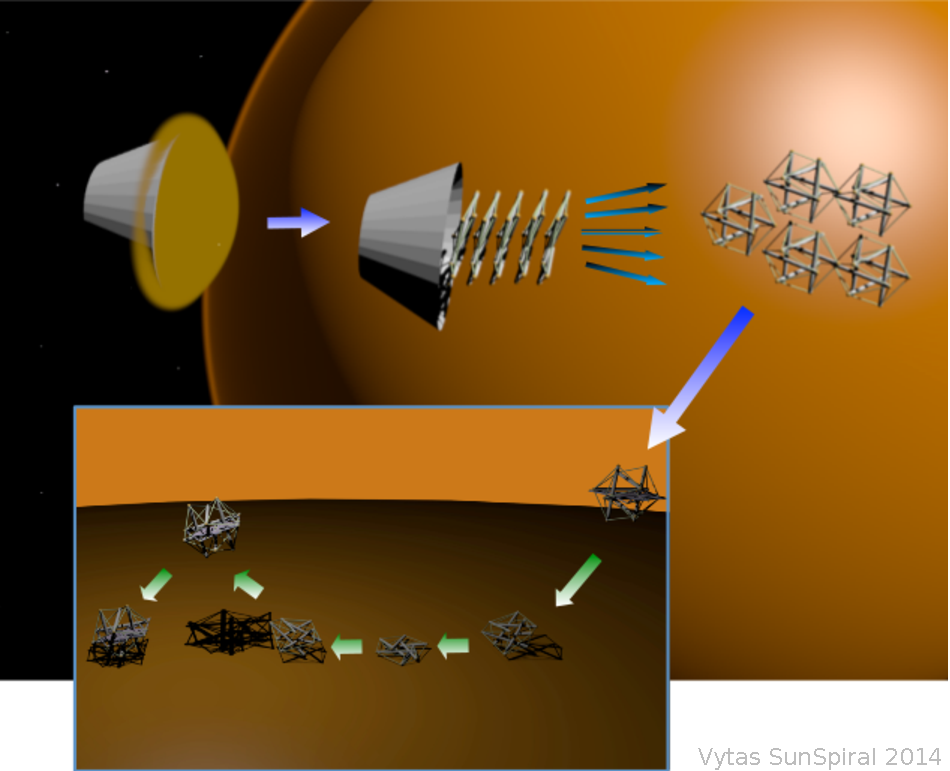
\includegraphics[width=0.5\textwidth]{tex/img/fig_aeroshell_summary} 
   \caption{{\em Tensegrity structures are composed of pure compression and tension elements. They can be lightweight, reliable, deployable, and efficient to manipulate. {\bf Mission Scenario} - Tightly packed set of tensegrities, expand, spread out, fall to surface of moon, then safely bounce on impact. The same tensegrity structure which cushioned the landing is then used for mobility to explore moons such as Titan and small asteroids.}}
   \label{fig:unpack}
\end{figure}

Tensegrity robots can facilitate an intriguing low-cost planetary exploration mission profile (see Figure~\ref{fig:unpack}) comprising of the following stages:  1) A set of tensegrity robots can be squeezed into a small launch platform; 2)  After initial atmospheric entry and ejection of the heat shield, they can automatically spring away from each other when released at their destination. 3) They ``bounce'' on impact reducing the need for final descent equipment, such as airbags; and 4) They can reorient themselves from landed position without addition reorientation hardware and efficiently move from scattered initial positions to perform sensor measurements; 5) They can survive significant falls and are resistant to being stuck, simplifying route planning and allowing for more aggressive exploration in the pursuit of science.

Once on the surface, tensegrity robots can perform an array of scientific analysis including soil and atmospheric composition, surface imagery and microscopic analysis. To further reduce complexity, sensors can be suspended on the interior of the tensegrity on cables attached to the nodes, or when appropriate even to the nodes themselves so that the sensors can be moved with movements of the structure itself, eliminating the need for separate sensor arms. In addition, environmental analysis can be performed in-situ at the landing site, at different local locations, or even at distant locations given a tensegrity robot's potential for efficient locomotion. The biggest advantages of this mission profile are:
\begin{enumerate}[leftmargin=.5cm]
\item The structure of the robot itself provides capability for deployment, landing (EDL), and mobility, reducing complexity, risk, and mass compared to using three separate systems.
\item Tensegrity robots are light-weight and can be packed tightly, reducing cost.
\item Can scale to multiple tightly packed robots to increase scientific coverage and reduce risk.
%TODO do we want to keep this statement on multiple robots?
\item Flexibility and modularity of robot design allows design reuse, reducing mission project risk.
\end{enumerate}

 \begin{figure}[h]
   \centering
   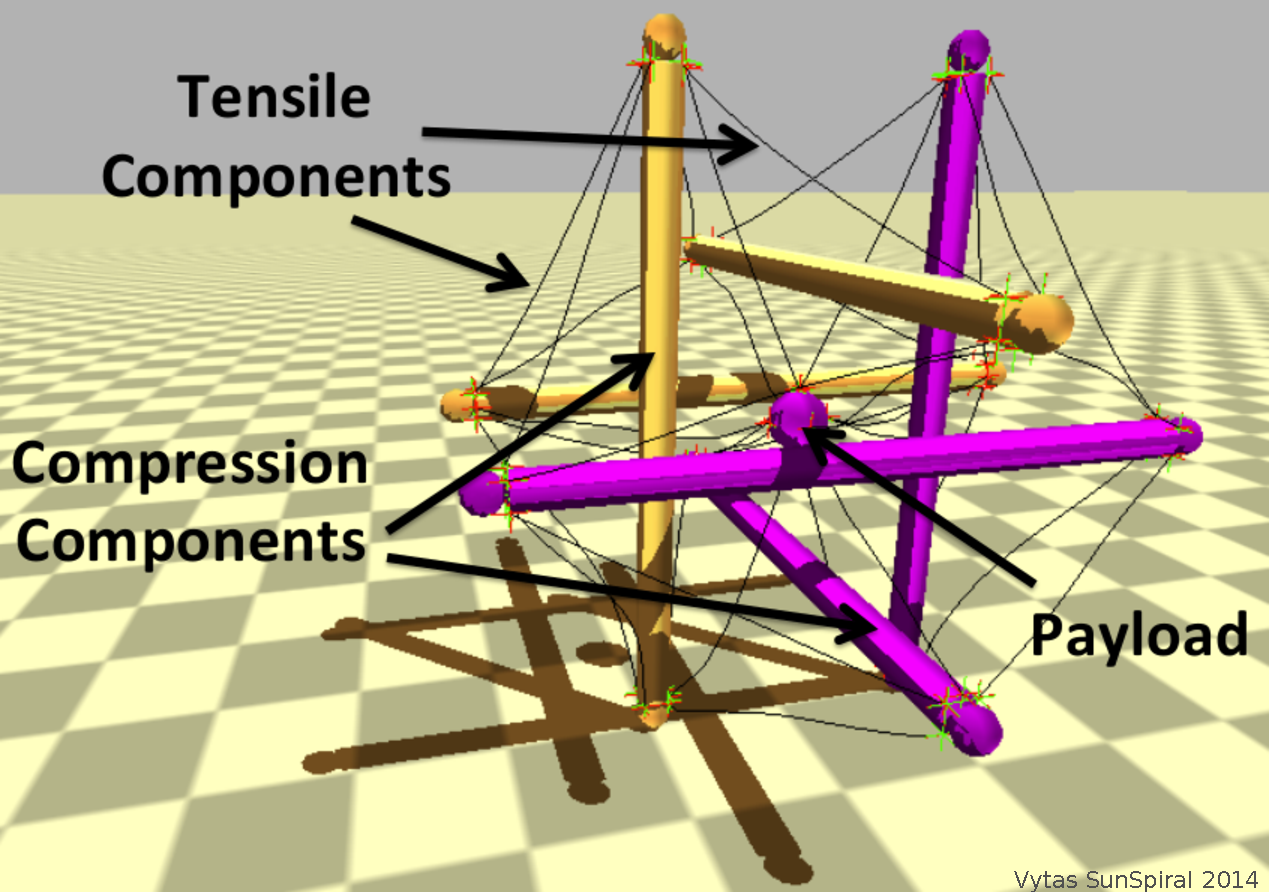
\includegraphics[width=0.5\columnwidth]{tex/img/fig_basic_diagram}
   \caption{{\em {\bf Tensegrity Structure.} Tensegrities are composed of pure tension and pure compression elements (e.g. cables and rods) as seen in this picture of a tensegrity robot from our physics based tensegrity simulator. They are light-weight, energy-efficient and robust to failures.}}
   \label{fig:basic_diagram1}
\end{figure}

\section{Goals}
\label{goal}
The main goals my project seeks to accomplish:

\begin{enumerate}[leftmargin=.5cm]
\item \textbf{Build a rolling tensegrity robot}\\
A physical hardware prototype of an untethered tensegrity robot to explore locomotion.
The robot will not only need to perform the basics for rolling, but will need to enable the next two goal items.
To achieve this, the robot will need significant mechanical power, distributed computation, and wireless communication.

\item \textbf{Open loop locomotion control}\\
Once the hardware prototype is built, an open loop control scheme will be developed.
The open loop algorithm will not change the control inputs to the system based on sensing outside of the robot.
This will demonstrate the system's ability to coordinate motion between it's distributed computation and collect data wirelessly.

\item \textbf{Closed loop "gait" control}\\
Once the system has proven the ability to locomote open loop, a closed loop algorithm will be developed.
The closed loop control will change the "gait", or locomotion pattern, of the robot to cope with sensed variations in terrain, e.g. changes in terrain grade or climbing over an obstacles.
To achieve this, research into the how much of the robot state is needed as well as various techniques to model and predict the environment by using the on board sensors.
\end{enumerate}

\chapter{Literature Review}

\section{Tensegrity Structures}
It is possible to design free-standing structures with axially loaded compression elements in a well crafted network of tensional elements.
Such an arrangement is called a tensegrity structure (tensile integrity). 
Each element of the structure experiences either pure axial compression or pure tension \cite{BuckminsterFuller1975}\cite{Snelson1965}.
The absence of bending or shear forces allows for highly efficient use of materials, 
resulting in lightweight, yet robust systems.

Because the struts are not directly connected, 
tensegrities have the unique property that externally applied forces distribute through the structure via multiple load paths. 
This creates a soft structure, for a soft robot, out of inherently rigid materials.
Since there are no rigid connections within the structure, there are also no lever arms to magnify forces. 
The result is a global level of robustness and tolerance to forces applied from any direction.

%Tensegrity structures are composed of axially loaded compression elements encompassed within a network of tensional elements, and thus each 
%element experiences either pure linear compression or pure tension.  As a result, individual elements can be extremely lightweight as there are no 
%bending or shear forces that must be resisted.  Because the struts are not directly connected, a unique property of tensegrity structures is how externally applied forces distribute through the structure 
%via multiple load paths, creating a system level robustness and tolerance to forces applied from any direction.  
%Because there are no rigid connections within the structure, there are also no lever arms to magnify forces.  Instead, all experienced forces act linearly on each structural element.  Combined with the ability to diffuse forces globally, 
This makes tensegrity robots inherently compliant and extremely well suited for physical interactions with complex and poorly modeled natural environments.  
Active motion in tensegrity robots can be performed by changing cable lengths in parallel, 
enabling the use of many small actuators that work together, rather than individual heavy actuators which work in series.  
There are also many indications that tensegrity properties are prevalent throughout biological systems, 
and the morphology of the SUPERball that we are studying, 
especially when carrying a payload, 
ends up bearing a striking resemblance to the nucleated tensegrity model of cell structure~\cite{Wang2009}\cite{Wang2001}.

\section{Prior Work in Tensegrity Robotics Design}
An important advantage of tensegrity structures with respect to general pin-jointed structures is their increased mass-efficiency due to a high fraction of tensile members.
Tensile members are generally more mass-efficient as they do not need to resist buckling.
A further advantage from a robotics perspective is that forces diffuse in a tensegrity.
There are no lever arms and torques do not accumulate at the joints as in a classic serial manipulator.
Forces distribute through multiple load paths, thus increasing robustness and tolerance to mechanical failure.

%advantages
%applications
The static properties of tensegrities have been thoroughly studied and some basic analysis is discussed in section \ref{modeling}.
On the other hand, few examples are known of truly dynamic motion of these structures.
Early examples of kinematic motion include the work at EPFL's IMAC laboratory~\cite{Fest2004}.
Skelton and Sultan introduced algorithms for the positioning of tensegrity based telescopes and the dynamic control of a tensegrity flight simulator platform~\cite{sultan2000tensegrity}.
Although there were some early efforts at MIT's CSAIL lab, it wasn't until the work of Paul and Lipson at Cornell University that the concept of tensegrity robotics became widespread~\cite{Paul2006a}.
Paul and Lipson were the first to study the properties of dynamic tensegrity structures in hardware and simulation.
A few years later Fivat and Lipson designed the IcoTens, a small actuated tensegrity icosahedron robot, but did not publish results.
In recent years, the BIER lab at the University of Virginia has been studying Central Pattern Generator based control for tensegrity based fish tails,
which is closely related to the control architectures proposed for SUPERball~\cite{Caluwaerts2013rsif,Bliss2012}.
Mirats-Tur has presented design and controls work on various other tensegrity morphologies that have been tethered or fixed to the ground~\cite{GraellsRovira2009,miratstur2011athree-dof}.
At Union College, Rieffel and colleagues are following an interesting line of work by considering vibration based actuation for small tensegrities~\cite{khazanov2014developing}.
Related work was presented by B\"ohm and Zimmermann, who demonstrated controlled locomotion of vibration driven tensegrity robots with a single actuator~\cite{bohm2013vibration}.
Finally, Shibata, Hirai and colleagues have developed pneumatically actuated rolling tensegrity structures~\cite{Shibata2009}. 
%goal

Building upon these works, the \SB{} project seeks to push forward the tensegrity robotics field and develop truly untethered, highly dynamic and compliant robots exploiting the aforementioned advantages.

\section{Tensegrity Robotics for Space Exploration}
%NASA is supporting research into tensegrity robotics to create robots with many of the same qualities that benefit biological systems.  
The high strength-to-weight ratio of tensegrity structures is very attractive due to the impact of mass on mission launch costs. 
Large tensegrity structures have been shown to be deployable from small compact configurations which enable them to fit into space constrained launch fairings.   
While the above qualities have inspired studies of deployable antennae and other large space structures~\cite{Tibert2002}, 
it is in the realm of planetary exploration that we see the most significant role for many of the unique force distribution qualities of tensegrity robots.  
The NIAC project currently funding this research~\cite{NIACfinalreport} specifically studies landing and surface mobility of tensegrities,
exploiting the controllable compliance and force distribution properties which make for reliable and robust environmental interactions.  

The main goal is to develop tensegrity probes with an actively controllable tensile network
 to enable compact stowage for launch, followed by deployment in preparation for landing. 
Due to their natural compliance and 
structural force distribution properties, tensegrity probes can safely absorb 
significant impact forces, enabling high speed Entry, Descent, and Landing 
(EDL) scenarios where the probe itself acts much like an airbag.  However, 
unlike an airbag which must be discarded after a single use, the tensegrity 
probe can actively control its shape to provide compliant rolling mobility 
while still maintaining the ability to safely absorb impact shocks that might 
occur during exploration.  This combination of functions from a single 
structure enables compact and lightweight planetary exploration missions 
with the capabilities of traditional wheeled rovers, but with a mass and 
cost similar or less than a stationary probe.   

Therefore, a large fraction of the overall weight (as measured at atmospheric entry) of a tensegrity mission can be used for the scientific payload 
due to the dual use of the structure as a lander and a rover. 
This allows for cheaper missions and enable new forms of surface exploration that utilize the natural tolerance to impacts of tensegrities~\cite{Vytas_IPPW_2013}.

% Because  of  the  limited  research  into  actuated  tensegrity
% robotics,   many   design   aspects   have   yet   to   be   carefully
% studied. To date, the majority of constructed tensegrity robots
% have  been  simple  prototypes  using  servo  motors,  limited
% sensing,  and  are  often  tethered  for  power  and  control  [5].
% Others have had fewer limbs than the SUPER ball, or have
% been  secured  to  the  ground  as  opposed  to  free-standing
% [6][7]. Some related approaches utilize tensegrity as part of a
% larger, more complicated system, but not as the primary loco-
% motion method [8]. Others have created designs that do not
% use direct cable actuation, as in the SUPER ball, but instead
% have  more  limited  forms  of  locomotion  through  vibration
% [9][10]. Finally, the most similar designs to the SUPER ball
% have not been engineered to specific design requirements nor
% have  the  advanced  sensing  framework  needed  for  controls
% testing [11]
%
% The  high  strength-to-weight  ratio  of  tensegrity  structures
% is very attractive due to the impact of mass on mission launch
% costs.  Large  tensegrity  structures  have  been  shown  to  be
% deployable from small compact configurations which enable
% them to fit into space constrained launch fairings. While the
% above qualities have inspired studies of deployable antennae
% and  other  large  space  structures  [12],  it  is  in  the  realm
% of  planetary  exploration  that  we  see  the  most  significant
% role  for  many  of  the  unique  force  distribution  qualities  of
% tensegrity  robots.  A  recent  NIAC  project  [13]  specifically
% studies  landing  and  surface  mobility  of  tensegrities,  ex-
% ploiting  the  controllable  compliance  and  force  distribution
% properties which make for reliable and robust environmental
% interactions.
% The   main   goal   is   to   develop   tensegrity   probes   with
% an  actively  controllable  tensile  network  to  enable  compact
% stowage  for  launch,  followed  by  deployment  in  preparation
% for  landing.  Due  to  their  natural  compliance  and  structural
% force  distribution  properties,  tensegrity  probes  can  safely
% absorb significant impact forces, enabling high speed Entry,
% Descent, and Landing (EDL) scenarios where the probe itself
% acts  much  like  an  airbag.  However,  unlike  an  airbag  which
% must  be  discarded  after  a  single  use,  the  tensegrity  probe
% can  actively  control  its  shape  to  provide  compliant  rolling
% mobility  while  still  maintaining  the  ability  to  safely  absorb
% impact  shocks  that  might  occur  during  exploration.  This
% combination  of  functions  from  a  single  structure  enables
% compact and lightweight planetary exploration missions with
% the capabilities of traditional wheeled rovers, but with a mass
% and cost similar or less than a stationary probe.
%
% Therefore, a large fraction of the overall weight (as mea-
% sured  at  atmospheric  entry)  of  a  tensegrity  mission  can  be
% used  for  the  scientific  payload  due  to  the  dual  use  of  the
% structure  as  a  lander  and  a  rover.  This  allows  for  cheaper
% missions  and  enable  new  forms  of  surface  exploration  that
% utilize the natural tolerance to impacts of tensegrities [14].
%
% Buckminster Fuller [1] and the artist Kenneth Snelson [2]
% initially  explored  tensegrity  structures  in  the  1960s.  Until
% the  mid-1990s  the  majority  of  tensegrity  related  research
% was  concerned  with  form-finding  [15]  and  design  analysis
% of  static  structure  [16][17].  More  recently,  active  control
% efforts  for  tensegrities  began  to  emerge  [18],  as  well  as
% descriptions  of  the  dynamics  of  tensegrity  structures  taking
% the connectivity pattern into account [17].
% The tensegrity principle allows for compliance and multi-
% path load distribution, which is ideal for physical interaction
% with  the  environment.  However,  these  aspects  also  present
% significant  challenges  to  traditional  control  approaches.  A
% recent  review  [19]  shows  that  there  are  still  many  open
% problems in actively controlling tensegrities, especially when
% interacting  with  an  environment  during  locomotion  or  ma-
% nipulation  tasks.  Though  work  has  been  done  to  control  a
% tensegrity  to  change  into  a  specified  shape  [20],  practical
% determination  of  the  desired  shape  itself  is  an  ongoing
% challenge.  Recently,  locomotion  of  icosahedral  tensegrity
% robots  through  body  deformation  was  demonstrated  [21].
% Other work has addressed collision between rigid tensegrity
% elements during control generation [22][23].
% The  approach  taken  by  the  NASA  Dynamic  Tensegrity
% Robotics  Lab  builds  on  this  by  developing  body  defor-
% mation  control  algorithms  based  on  central  pattern  gen-
% erators  [24][25],  distributed  learning,  reservoir  computing,
% and  genetic  algorithms  [26],  instead  of  traditional  linear
% and  nonlinear  systems  approaches.  To  date,  our  approach
% has  shown  promising  results  at  productively  harnessing  the
% potential  of  complex,  compliant,  and  nonlinear  tensegrity
% structures.

% \section{Motivation an Goal}

\chapter{Modeling and Model Validation}
\label{modeling}

\begin{figure}[thpb]
      \centering
      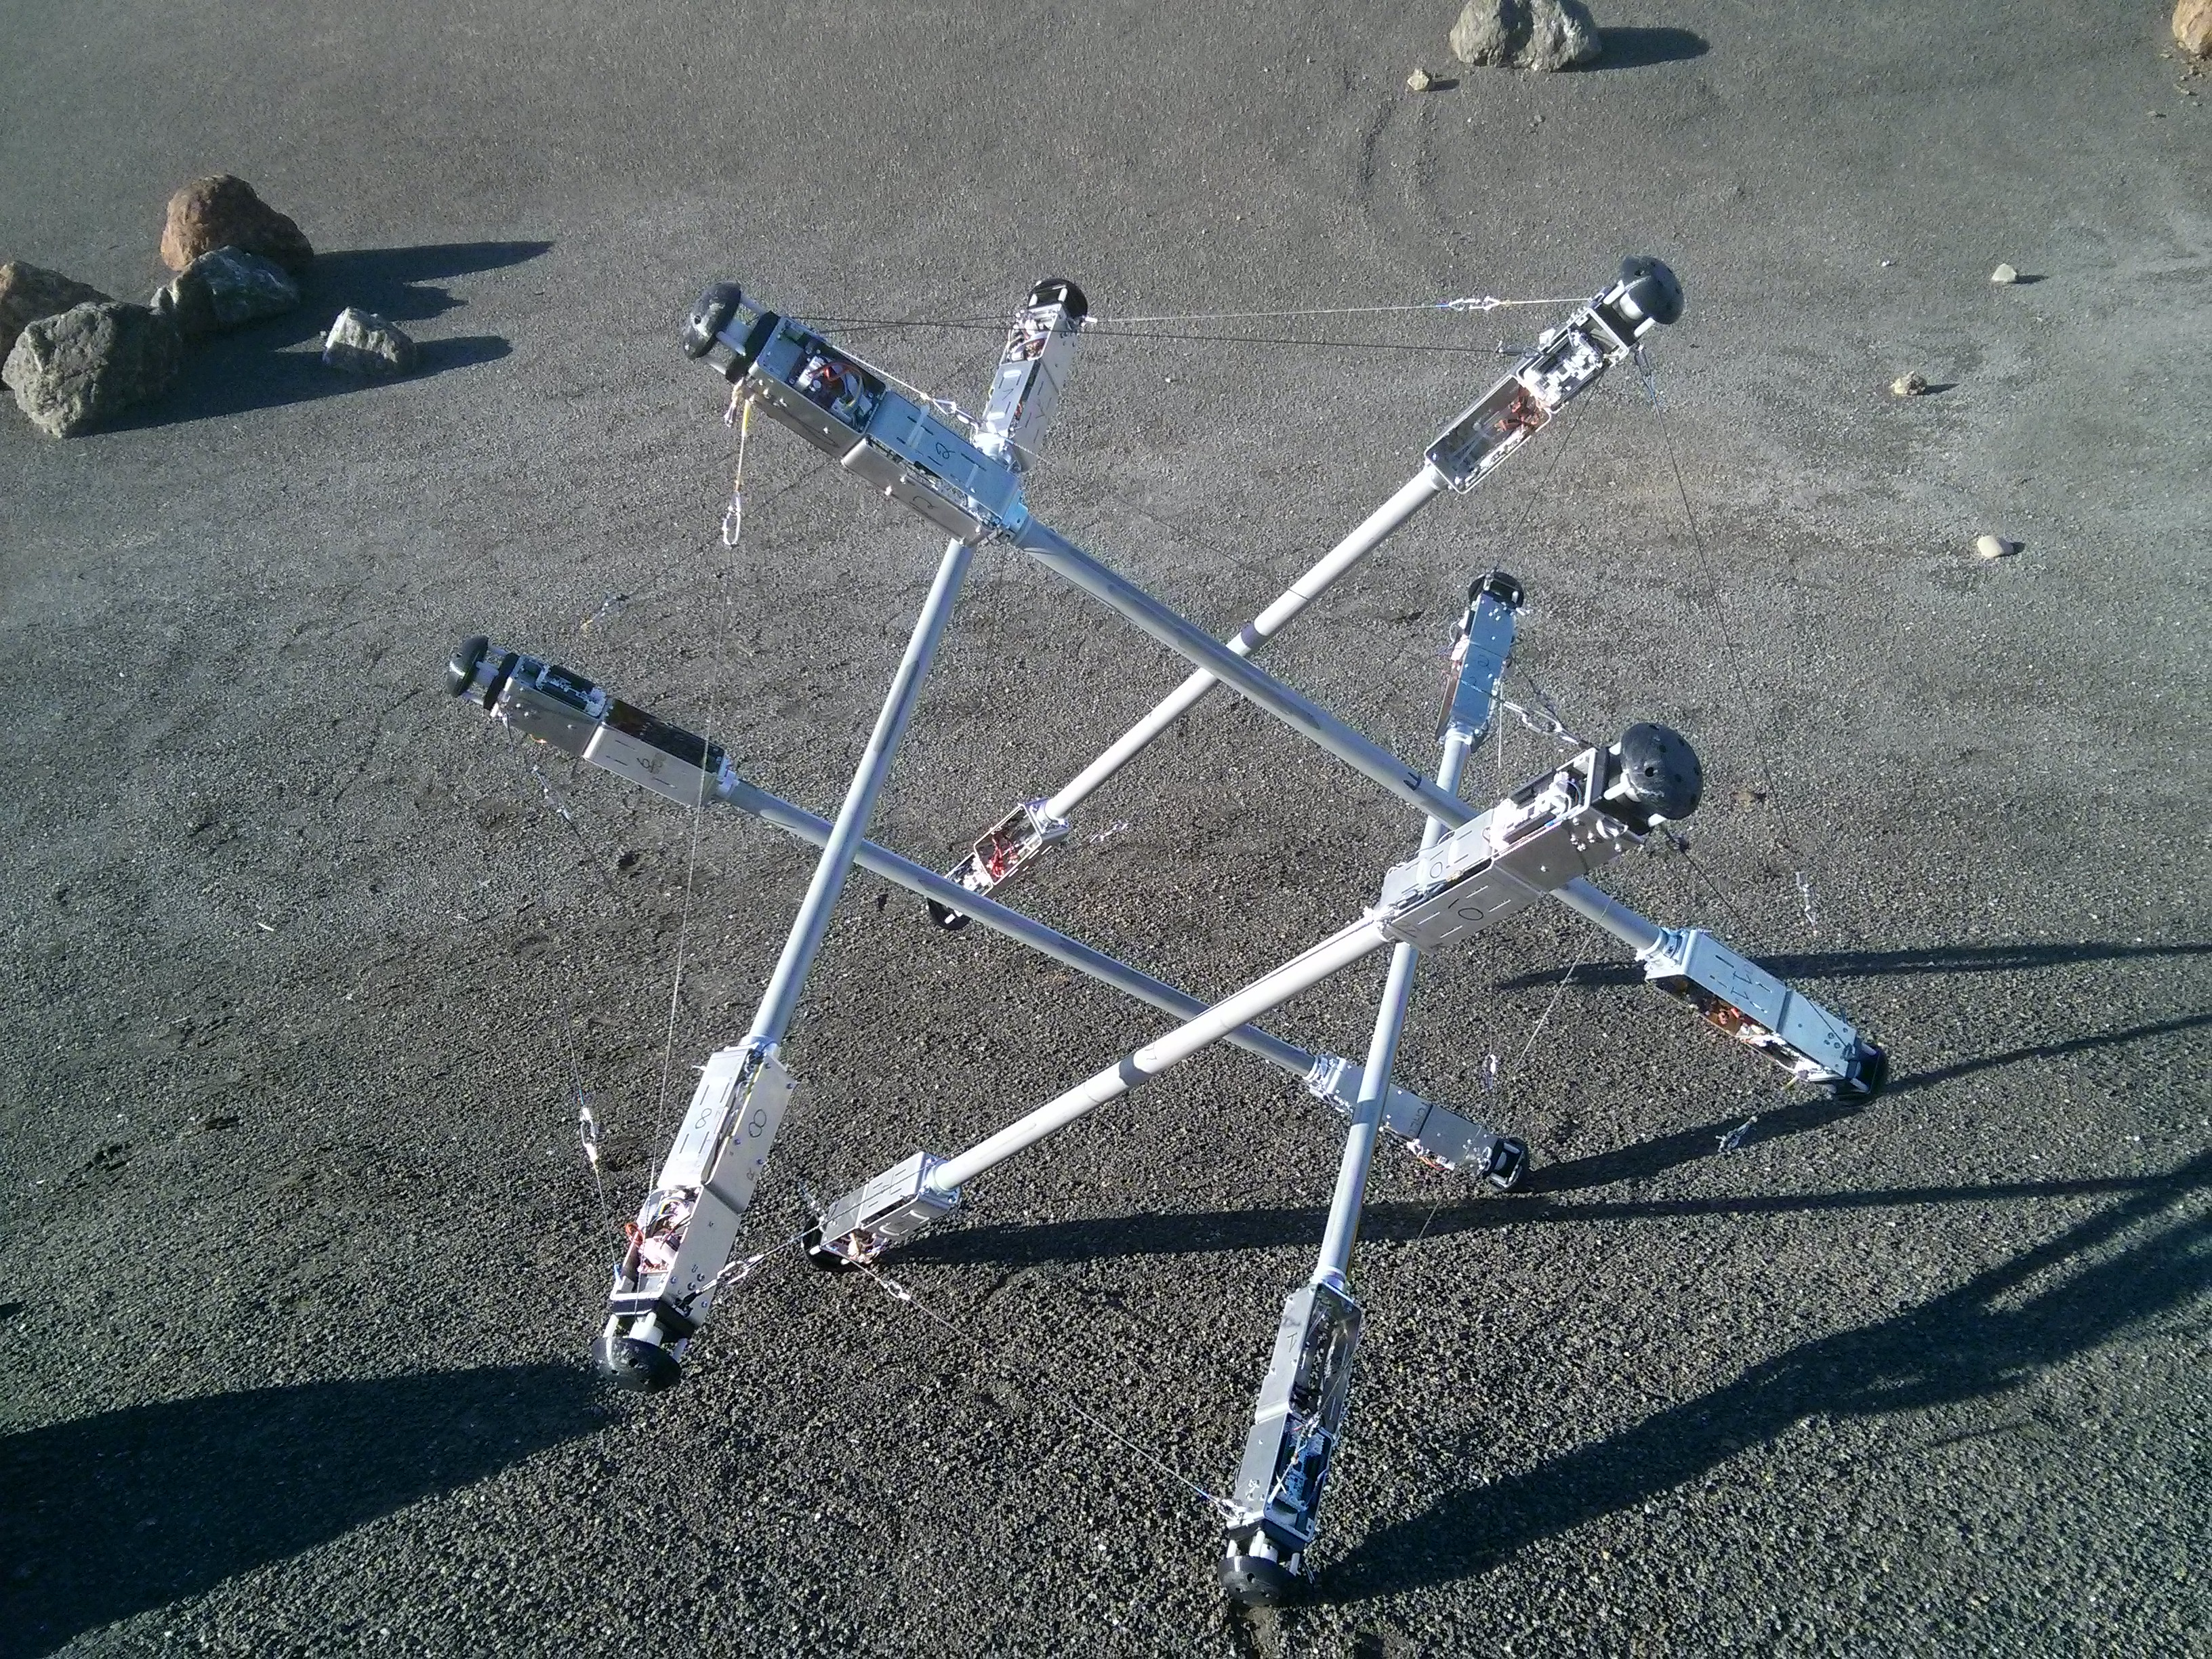
\includegraphics[width=0.8\columnwidth]{tex/img/superball_roverscape2_cropped.jpg}
      \caption{SUPERball, fully assembled, in the NASA Ames Research Center Roverscape.}
      \label{fig:SB}
\end{figure}

As part of our research for the NASA Innovative Advanced
Concepts  (NIAC)  program,  we  are  developing  the \SB{} (Spherical Underactuated Planetary Exploration Robot),
which is a compliant icosahedron tensegrity robot designed
for   planetary   landing   and   exploration, seen in figure \ref{fig:SB}.   Tensegrity   robots
are  soft  machines  which  are  uniquely  able  to  compliantly
absorb  forces  and  interact  with  unstructured  environments.
However, instead of engineering a single new robot, we have
chosen  to  develop  a  fundamentally  reusable  component  for
tensegrity  robots  by  creating  a  modular  robotic  tensegrity
strut which contains an integrated system of power, sensing,
actuation, and communications. The purpose is to enable the
exploration of the wide range of possible tensegrity robotic
morphologies  by  simply  combining  the  robotic  struts  into
new systems.

Though there is much prior work in a variety of theoretical
areas for tensegrities, engineering knowledge of constructing
practical  tensegrity  robots  is  limited.  Since  a  staggering
variety  of  different  tensegrity  structures  can  be  constructed
from  collections  of  simple  sticks  and  strings, we have made it a priority
to develop self-contained robotic tensegrity struts which can
be  used  to  explore  and  build  a  wide  range  of  tensegrity
robots  simply  by  combining  them  into  novel  structures.
Our  designs  are  driven  by  experimental  results  obtained
from  a  previous  prototype,  ReCTeR  (Reservoir  Compliant
Tensegrity Robot) in combination with simulation results of
our validated tensegrity simulator NTRT (NASA Tensegrity
Robotics Toolkit)~\cite{2917079}\cite{Caluwaerts2013rsif}.

In  order  to  develop  SUPERball  from  ReCTeR's  design
limitations as well as our lab’s need for rapid experimentation
of  various  tensegrity  configurations  and  morphologies,  we
came  up  with  a  modular  tensegrity  platform  to  research
large  scale  robotic  tasks;  e.g.  a  tensegrity  planetary  probe
to explore Saturn's moon Titan.
%Our lab obtained design requirements through an iterative
%approach  involving  NTRT  and  ReCTeR.  As  we  validated  our  NTRT  simulator  by  experimental  validation
%with  ReCTeR~\cite{Caluwaerts2013rsif} and can  now  quickly  evaluate  various
Our lab obtained design requirements through an iterative approach with validated our NTRT simulator by experimental comparison with ReCTeR~\cite{Caluwaerts2013rsif}.
We now can quickly  evaluate  various
tensegrity  configurations  in  simulation  to  find  optimal  mechanical  design  goals.  In conjunction with the  NTRT  solver,  we  also
incorporated  results  obtained  with  our  (open  source)  Euler
Lagrange solver based on Skelton's work~\cite{Skelton2009} and measurements on ReCTeR.
The initial design requirements obtained from the NTRT simulations, refined designs after a first prototype build, and how these compare to other tensegrity robotic systems are given in Table \ref{design_req}.


\begin{table*}[ht]
%\begin{minipage}[t][\linewidth]{
\caption{\SB{} and Related Robots Design Overview.} 
\label{design_req}

\begin{center}%
\resizebox{\columnwidth}{!}{%
\begin{tabular}{lrrrcrrrrrrr}
%\hline
&$\bm{l_{strut}}$ & $\bm{\Delta l_{act}}$ & $\bm{k_{passive}}$ & \bf{tethered?} & \bf{control} & $\bm{f_{act}}$ & \bf{\#act.} & \bf{mass} & \bf{sensors} &\bf{actuators} &\bf{ref.} \\ \hline \hline
\bf{Pneumatic}&\SI{.57}{m} & - & - & Y & open loop & \SI{800}{\newton} & \num{24} & \SI{3.3}{\kg}& none & McKibben& \cite{Koizumi2012b} \\
\bf{ReCTeR}&\SI{1}{m} & \SI{0.3}{\metre} & \SI{28.4}{\newton\per\metre} & N & closed loop & \SI{12}{\newton} & \num{6} & \SI{1.1}{\kg} & F, L, IMU & DC & \cite{Caluwaerts2013rsif} \\
\bf{Rapid Proto Kit}&\SI{.69}{m} & \SI{0.005}{\metre} & \SI{1193}{\newton\per\metre} & N & open loop  & $<$\SI{45}{\newton} & \num{24} & \SI{2.7}{\kg}& none & linear DC &\cite{kim2014rapid} \\
\bf{\SB{} 2014}&\SI{1.5}{m} & \SI{0.2}{\metre} & \SI{613}{\newton\per\metre} & N & closed loop & \SI{140}{\newton}  & \num{12} & \SI{9}{\kg}& F, L, $\tau$, IMU & BLDC& \\
\bf{\SB{} 2015}&\SI{1.7}{m} & \SI{0.42}{\metre} & \SI{998}{\newton\per\metre} & N & closed loop & \SI{250}{\newton} & \num{12} & \SI{21}{\kg} & F, L, $\tau$, IMU & BLDC& 
%Tensegrity Kit 
%\SB{} ICRA 2014 &$1.5\mbox{m}$ & $0.26 {\mbox{m}}/{\mbox{s}}$ & $500 \mbox{N}/\mbox{m}$ & $100\mbox{Hz}$ & $3 \mbox{Nm}$ \\
%\SB{} ICRA 2015
%\hline

\end{tabular}
}
\end{center}
\bigskip
\fontsize{10pt}{12pt}\selectfont
The variable $l_{strut}$ indicates the length of a strut, $\Delta l_{act}$ is the nominal spring-cable retraction length in tension, $k_{passive}$ is the linear stiffness coefficient of a passive spring-cable (or active spring-cable if fully actuated), tethered indicates if the robot is powered externally or by internal systems, control indicates whether sensor feedback is used, $f_{act}$ is the nominal actuated spring-cable tension and \#act. is the number of actuators. In the sensors column, F represents a linear force sensor (for cables), L is cable length sensor (in the form of motor encoders), $\tau$ represents a torque sensor for motors, and IMU represents an accelerometer/gyroscope inertial motion sensing unit. Actuators are specified as DC motors or brushless DC (BLDC) motors. The SUPERball 2014 values are revised original design requirements based on NTRT simulations, and changed to the 2015 values after additional detail design. %

\vspace{-0.2cm}

%\end{minipage}
\end{table*}

The work presented here is work verifying our in house tensegrity simulators.
In order to achieve this, the group decided to use a \SB{} like structure with a center payload.
This is believed to be closer to the proposed build profile of a real tensegrity probe, where the main science modules will be contained within the payload.
Protecting this science payload is the main goal for and EDL scenario.
Figure \ref{fig:NTRT_SB} shows a 3-D representation of \SB{} with a payload generated within NTRT.

\begin{figure}[thpb]
      \centering
      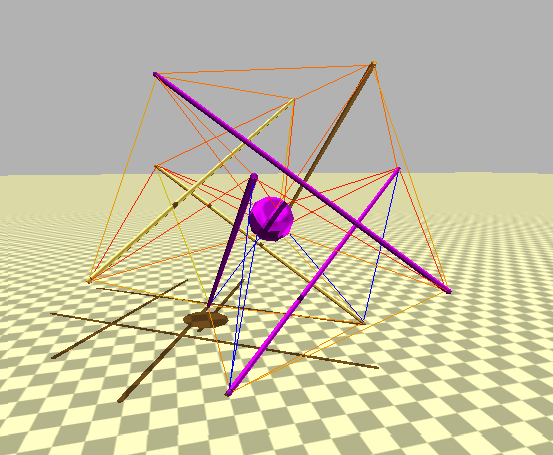
\includegraphics[width=0.8\columnwidth]{tex/img/1.png}
      \caption{SUPERball with a payload modeled within NTRT.}
      \label{fig:NTRT_SB}
\end{figure}

\section{Euler-Lagrange Model}
In order to verify the simulation results produced by our NTRT simulator, we decided to compare the behavior of the NTRT to a published analytic model for tensegrity systems.
We choose to use Skelton's dynamic equations because it is a well accepted and used model.
It may be found in his \emph{Tensegrity Systems} book \cite{skelton_tensegrity_2009} which is based on his work in \cite{skelton2005dynamics}.
In order to solve the dynamic equations with interactions with the environment, an Euler-Lagrange approach is used as well as Skelton's constrained class one structure.
The lagrange equation for a constrained rod is given by
\begin{equation}
\label{eq:lagrange}
L = T - V - c
\end{equation}
where
\begin{align}
\mathbf{b} &= l^{-1}(\mathbf{n}_{j}-\mathbf{n}_{i})\label{eq:normalizedVector}\\
c &= \frac{\mathbf{J}\xi}{2}(\mathbf{b}^{T}\mathbf{b}-1)\label{eq:constraint}
\end{align} 
Equation \eqref{eq:normalizedVector} is the normalized vector of a rod with \(\mathbf{n}_{i,j}\) the nodal positions in \(R^3\), and equation \eqref{eq:constraint} contains the lagrange multiplier \(\xi\) to keep \eqref{eq:normalizedVector} constrained.
\(\mathbf{J}\) is also defined as the inertia matrix for a one dimensional rod in three dimensional space.
In order to define the system of \(k\) rods we need to define a combined Lagrangian as
\begin{equation}
\mathbf{L} = \sum_{i=1}^{k} L_{i}\label{eq:combinedLagrangian}
\end{equation}
where \(L_{i}\) is the Lagrange function for each rod.
Using the approach outlined in Skelton's book for deriving the equations of motion, we can then derive the configuration matrix
\begin{equation}
\mathbf{Q} = \begin{bmatrix}
	\mathbf{R} & \mathbf{B}
	\end{bmatrix}\label{eq:configMatrix}
\end{equation}
where \(\mathbf{R}\) and \(\mathbf{B}\) are matrices containing the translational and rotational vectors, respectively. They have the form
\begin{align}
\mathbf{R} &= \begin{bmatrix}
	\mathbf{r}_{1} & \cdots & \mathbf{r}_{k}
	\end{bmatrix}\label{eq:transR}\\
\mathbf{B} &= \begin{bmatrix}
	\mathbf{b}_{1} & \cdots & \mathbf{b}_{k}
	\end{bmatrix}\label{eq:rotB}
\end{align}
Also using the procedure to derive generalized forces within Skelton's book, the systems's generalized force equations are computed as
\begin{equation}
\mathbf{F}_{\mathbf{Q}} = \begin{bmatrix}
	\mathbf{F}_{\mathbf{R}} & \mathbf{F}_{\mathbf{B}}
	\end{bmatrix}\label{eq:generalizedForce}
\end{equation}
with
\begin{align}
\mathbf{F}_{\mathbf{R}} &= \begin{bmatrix}
	\mathbf{f}_{\mathbf{r}_{1}} & \cdots & \mathbf{f}_{\mathbf{r}_{k}}
	\end{bmatrix}\label{eq:gForceR}\\
\mathbf{F}_{\mathbf{B}} &= \begin{bmatrix}
	\mathbf{f}_{\mathbf{b}_{1}} & \cdots & \mathbf{f}_{\mathbf{b}_{k}}
	\end{bmatrix}\label{eq:gForceB}
\end{align}
Finally, we can define the resulting equations of motion in a compact form as
\begin{equation}
(\ddot{\mathbf{Q}} + \mathbf{Q}\mathbf{\Xi})\mathbf{M} = \mathbf{F}_{\mathbf{Q}}\label{eq:compactForm}
\end{equation}
where
\begin{align}
\mathbf{\Xi} &= diag\begin{bmatrix}
	0,\cdots,0,\xi_{1},\cdots,\xi_{k}
	\end{bmatrix}\label{eq:lagrangeMatrix}\\
\mathbf{M} &= diag\begin{bmatrix}
	m_{1},\cdots,m_{k},J_{1},\cdots,J_{k}
	\end{bmatrix}\label{massMatrix}
\end{align}
This approach was then implemented in Python utilizing a 4th order Runge-Kutta formula for solving the system of ordinary differential equations.  
In order to implement a gravitational field, a force distribution function is applied along the length of each rod and calculated as a nodal force depending on the given density of the rod.
This external force is then applied to the nodes during each time step, simulating a gravitational field.

\section{Detailed Impact Simulations and Cross-Validation Using Two Simulators}
The NTRT simulator is the most general purpose, allowing us to explore control algorithms and complex environmental interactions, but it is an iterative discrete solver that we were concerned might not be providing accurate answers.  The E-L solver, on the other hand, has a much stronger analytical basis and should provide very accurate answers, but is limited because some of the nodes (rod ends) must be constrained and locked into place.  This is unrealistic for the deformation caused during landing, and makes it an inappropriate choice for mobility and controls research.
If ground contact forces are incorporated into the E-L solver and code optimization implemented, it could be used in conjunction with a unscented kalman filter for state estimation propogation.
This tool could then be used to develop online learning algorithms for mobility research.

In this section, we compare the NTRT simulator and E-L solver at the moment of impact with the ground. 
The simulations are compared at the moment of impact with the ground because our implementation of the analytic E-L solver requires select nodes to be constrained.
We setup the structure so that it is barely in contact with the ground and is in balance at time equal to 0. 
In both simulations, we add an initial velocity equal to the terminal velocity of Titan, and compared each vertical trajectory, vertical velocity, and vertical acceleration of the payload. 
Since the structure's horizontal speed is zero at the beginning and the structure is symmetrical, the payload's horizontal components of position, velocity and acceleration are zero. 
As it can be seen in the Figures \ref{fig:vsPosition} and \ref{fig:vsVelocity}, both simulators closely match and generate the same results for position and velocity with the error margin close to zero. 
Comparing the accelerations generated by two simulators (Figure \ref{fig:vsAccelerations}), it can be seen that there is a bigger difference. 
The reason behind this difference is the fact that NTRT uses Bullet, which is a discrete time simulator and accelerations are calculated using two point estimations from velocities at the timestep before.  Yet, even with these differences in accelerations, our conclusion at the end of the comparison is that both simulators showed the same basic dynamics and their results were close enough that we could move forward using the more general purpose NTRT Simulator for our controls, mobility, and landing experiments.


\begin{figure}[htb]
   \centering
   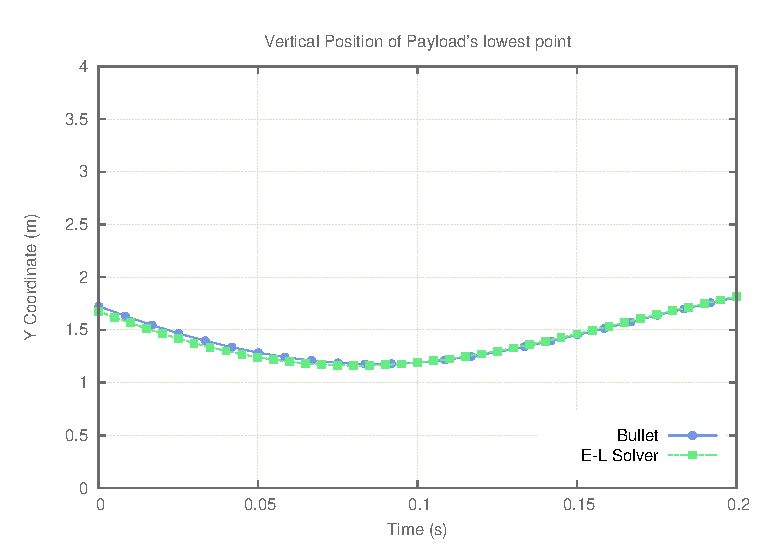
\includegraphics[width=0.8\columnwidth]{tex/images/landing/bulletVsEL/SimVsEL}
   \caption{NTRT vs EL: Vertical Position}
   \label{fig:vsPosition}
\end{figure}

\begin{figure}[htb]
   \centering
   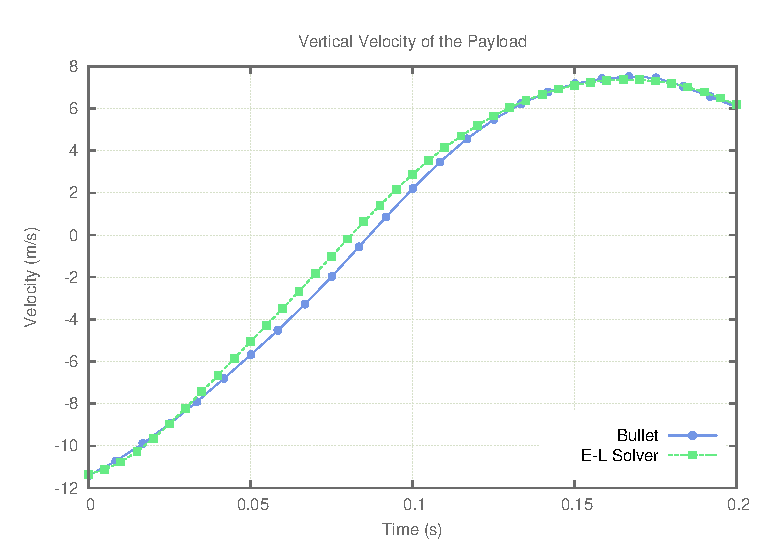
\includegraphics[width=0.8\columnwidth]{tex/images/landing/bulletVsEL/Velocities}
   \caption{NTRT vs EL Vertical Velocity}
   \label{fig:vsVelocity}
\end{figure}
\begin{figure}[htb]
   \centering
   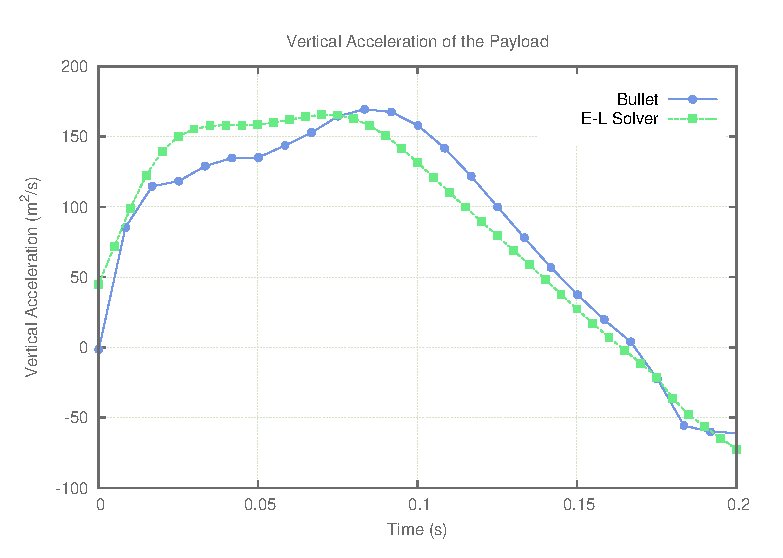
\includegraphics[width=0.8\columnwidth]{tex/images/landing/bulletVsEL/VelocityDerivatives_SimVsEL}
   \caption{NTRT vs EL Vertical Acceleration}
   \label{fig:vsAccelerations}
\end{figure}


\section{Simulated Drop Tests and Payload Protection}

Finally, we performed extensive analysis on drop tests and the protection provided to a payload.   As expected, we found that by varying the rod lengths, which impacts the stroke distance for the payload to decelerate, we could control the maximum deceleration experienced by the payload while ensuring that it did not collide with the ground or structure.  For example, with rods of 1.5 meters in length, our payload experienced a max deceleration of 21.4G when landing at 15 m/s. In figure \ref{fig:rodvsG} we show the results of a series of drop tests with different rod lengths and show the resulting maximum deceleration and forces experienced in the tension members.   As can be seen from these graphs, even for reasonable rod lengths, the maximum G's are acceptable for most instruments, and the maximum forces experienced by the cables are easily within ranges that can be engineered for.  In all tests we kept the total system mass constant, at 100kg (which is 70kg for the payload and 5kg per rod) in order to highlight the impact of structural geometry and rod length.  For the tension members we used spring constants of 44 kN/m for the cables around the perimeter and 10 kN/m for the cables attached to the payload.  Also, the results in Figure \ref{fig:rodvsG} were found using the landing orientation of 35 degrees around X axis and 45 degrees around Z axis, which we selected from our orientation studies discussed below. 

\begin{figure}[htbp]
\centering
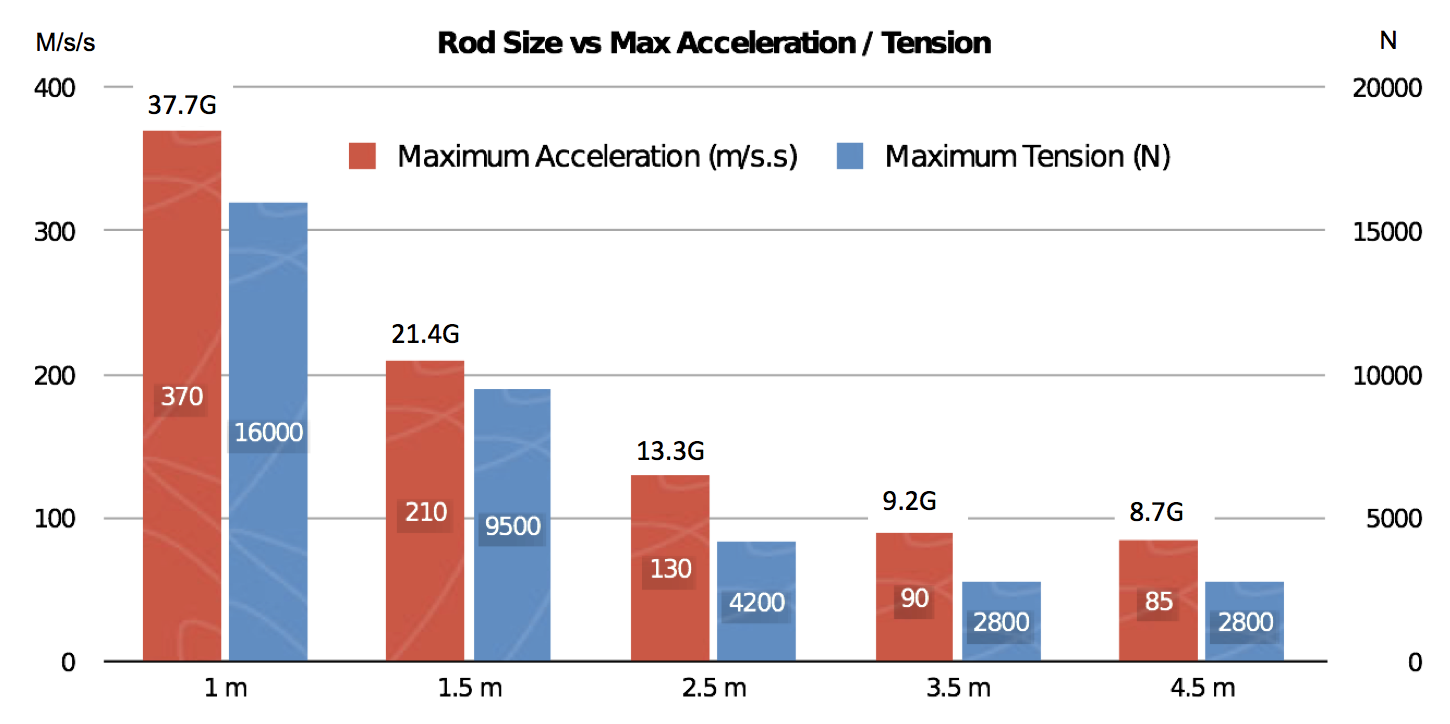
\includegraphics[width=0.8\columnwidth]{tex/images/rodvsG_fixed2}
\caption{{\em {\bf Landing Forces Study}. This shows how rod length impacts maximum deceleration of the payload and  the maximum forces experienced by the tension cables.  All tests were conducted with a landing velocity of 15 m/s onto a hard surface.}}
\label{fig:rodvsG}
\end{figure}

A very interesting point to consider is that the mass of our system will grow in a linear fashion with the length in the rods, while providing increasing payload protection.  On the other hand, the mass of airbags increases with the square of the radius, which is one of the reasons that the MSL rover, with its increased size and mass, had to switch from the airbag approach to the more complex Sky Crane approach.  While this study has focused on small light-weight mission concepts, we expect that there are compelling advantages to scaling up to handle larger payloads and we look forward to studying this further in the future.

\section{Landing Orientation Studies}
In order to study how landing orientation affects payload decelerations and impact events, we conducted a systematic study of landing orientations.  Since we wanted to get meaningful data, even for bad orientations, we used a larger tensegrity with 4 meter rods so the data wouldn't saturate.  Our success criteria for this study was that the decelerations had to stay under an upper limit of 25G deceleration of the payload, and the payload had to avoid collision with the ground or parts of the tensegrity structure.  Figure \ref{fig:landingHeatMapRot} shows the orientations that were safely within these criteria (black) or failed one or both of the criteria (colored).  By using a simple trailing streamer during descent it would be possible to control landing at an optimal orientation and enable the use of smaller structures with shorter rods because the orientation control would maximize the available stroke for the payload to decelerate within the structure.  Conversely, we can use these studies to know what the worst possible landing scenario will be and choose a structure size which will allow safe landing at any orientation.

\begin{figure}[htbp]
   \centering
   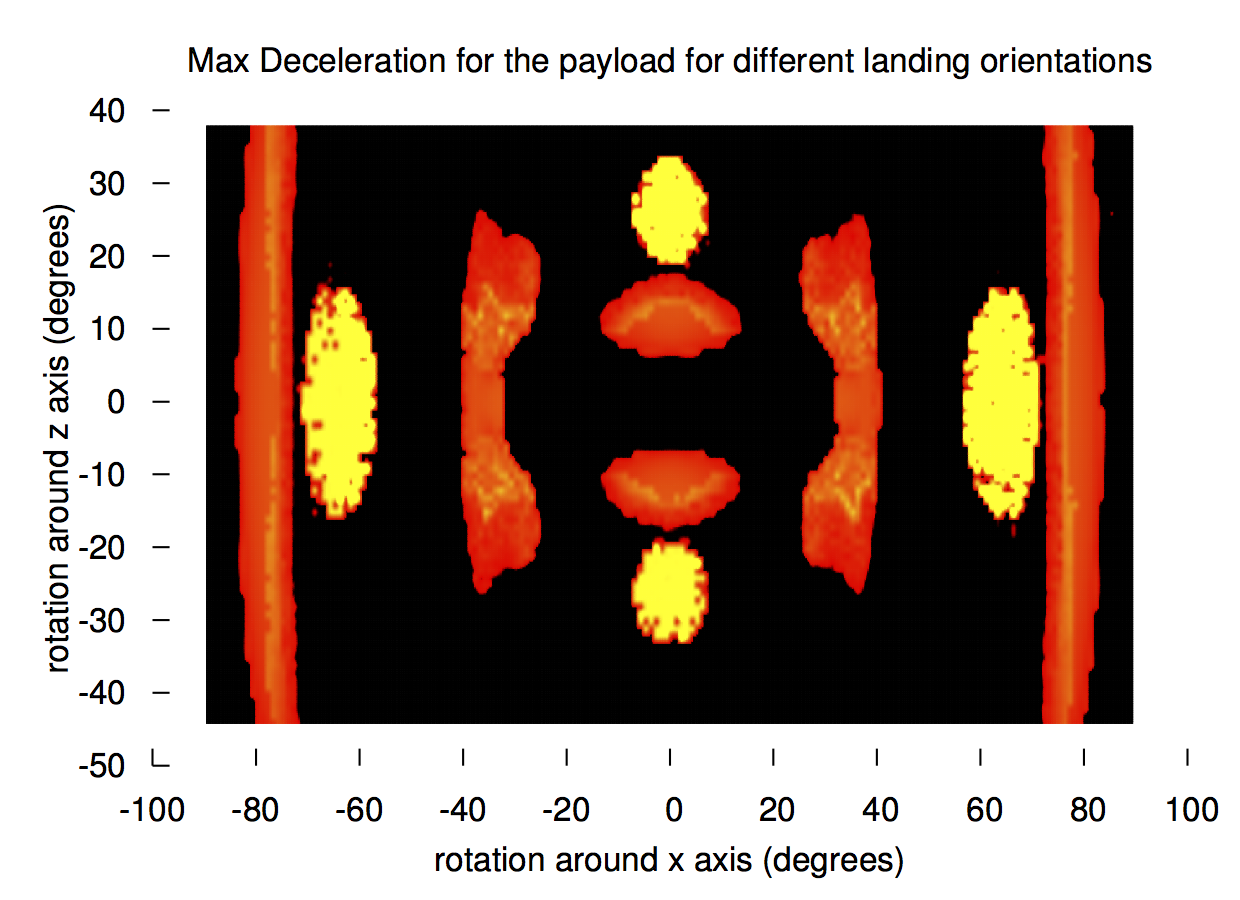
\includegraphics[width=0.8\columnwidth]{tex/images/landing/landingHeatMapRot.png}
   \caption{\em Heat map of the maximum acceleration that the payload encounters for all possible landing orientations. Black areas are safe, colored areas are where the payload does not meet one or both success criteria.}
   \label{fig:landingHeatMapRot}
\end{figure}


\section{Conclusions from Simulation Experiments}
In our landing analysis we developed and cross-validated two different simulation methods that allowed us to explore the capabilities of a tensegrity structure to absorb the forces of landing and to simultaneously protect a delicate payload.  This analysis confirmed that indeed it is possible to do so using a 6-bar tensegrity probe while maintaining maximum decelerations experienced by the instrument-containing payload to forces less than 25G, despite the structure landing at 15 m/s (which is greater than terminal velocity on Titan).   Comparing this to the Huygens probe's landing acceleration of \(32G\) \cite{lorenz1994huygens}, the tensegrtiy probe will have a \(43\% \) reduction in \(G\) forces experienced by the scientific payload, despite the Huygens probe's use of parachutes to land at 1/3 of the speed of our tensegrity probe.

\chapter{Mechatronic Design}

An ideal tensegrity system, either robotic or static, is a collection of rigid compressive elements suspended within a network of tensioned cables. 
For a robotic tensegrities without a payload, the actuation and supporting electronics would be logically designed into the compressive elements. 
Making each compressive element identical will also make the over all design and support of the entire tensegrity robot simplier. 
For SUPERball, each compressive element would be comprised of three parts: two identical end caps and a piece of tube stock. 
The end cap was designed 

\section{Mechanical}
Write about the mechanical design of SUPERball. Make sure to give credit where credit is due.

B.  Mechanical Design
SUPERball  is  an  icosahedron  tensegrity  structure  com-
prised  of  12  motors  at  the  end  of  the  robot’s  6  rods.  Each
rod  is  comprised  of  three  main  elements,  2  modular  end
cap  assemblies  containing  all  the  mechanical  and  electrical
systems   and   a   connecting   aluminum   tube   as   a   support
structure. The main structural elements of the end caps were
kept  simple  and  in  sections  to  enable  each  end  cap  to  be
modular  as  well  as  self  contained  so  that  the  end  cap  may
be removed from the connecting rod as one whole unit. The
end  caps  are  held  onto  the  connecting  rods  by  a  simple
tube  collar  for  easy  removal.  There  are  5  sections  to  the
modular end cap which are, a spring holder, battery holder,
motor and electronics element, cable actuation section, and a
ground contact section. These sections as they are designed
for SUPERball are shown in Fig. 4. Each of these 5 sections
can  be  removed  from  the  rod  as  a  full  sub-assembly  and
replaced with a new component, increasing the versatility of
each rod.
A  lesson  learned  from  ReCTeR  was  that  externally  ex-
posed springs are not ideal for a robotic system. The exposed
springs get caught on objects and the assumption of massless
cables  can  no  longer  be  applied.  On  the  modular  end  cap
for SUPERball, an enclosed compression spring system was
developed  to  alleviate  these  issues.  Compression  springs
were chosen so that during any unknown impact, the springs
would not plastically deform. For SUPERball, a spring with
a spring constant of
613
N=m
is attached to a passive cable
element  and  a
2850
N=m
spring  is  attached  to  an  actuated
cable.  The  passive  spring  has  a  much  higher  compressive
range to allow for pretension to be instated into the passive
springs.  A  working  prototype  of  our  spring  holder  system
can be seen in Fig. 5.

\section{Electrical}
Write about the electronic board used on SUPERball.\\

SUPERball  was  developed  with  distributed  controls  in
mind.  Each  rod  end  cap  houses  two  control  boards,  one
for  motor  driving  and  one  for  handling  sensing  and  com-
munications. Each board hosts a Microchip dsPIC33EP. The
motor driver is a BLDC/PMSM driver board capable of block
commutation and sensorless sinusoidal control. Each sensor
board is equipped with an ADC
(24bit Analog AD7193)
and
9 DOF IMU data
(MPU6000 and MAG3110)
.
Two custom force sensors were developed for the SUPER-
ball, a reaction torque sensor and a compression force sensor.
Fig. 6 shows the reaction torque sensor. It is a symmetrical
four  arm  cross  design  with  the  half  bridge  located  in  the
center of each arm. This sensor, along with the compression
sensors and current sensors allow us to implement high level
control schemes such as impedance control in which the full
state of the mechanical and electrical system must be known.

- Untethered electronics
- 

To this end, we tried to develop electronics which where extensible for various communications
Another driving parameter was the ability to drive the 100W BLDC Maxon motors chosen from the initial iterative design.
These two main design criteria governed our prototype to implement four separate electronic boards per end cap.
Three boards are custom designed PCBs and the fourth is an ARM based computer called Beagle Bone Black.
Each custom PCB is designed for very different purposes: A board to condition sensor data and run real-time control loops, a board to condition and distribute a 5.5V electronic power rail and a 24V motor power rail, and a board to control the 100W BLDC motor. 
The boards are simply named by their main purpose, thus Sensor, Power, and Motor board, respectively.

\subsubsection{Sensor Board}
The sensor board was originally designed as the main processing unit on an end cap for SUPERbal. 
However, the design and building process has lead to the coupling of the sensor board with a Beagle Bone Black.
These two versions are dubbed v1 and v2, respectively.
I will first write about v1 of the sensor board, then follow up on how v2 was changed.\\

The main processing unit on each sensor board is Microchip's dsPIC33EP128GP506, a 16 bit microcomputer running at 140MHz. 
Besides the designer's familiarity with this family of microcomputers, the dsPIC33E chips feature multiple Universal Asynchronous Receiver/Transmitter (UART), Serial Peripheral Interface (SPI), and Inter-Integrated Circuit (I2C) communication modules. 
The dsPIC33E also features an ECAN modules with 2.0B support, a 12 bit Analog to Digital Converter, and four Direct Memory Access (DMA) channels. 
All these moudles coupled with almost complete pin to peripheral pin remapping made the microcomputer a solid choice for our sensor board. 

\section{Communication and Data Flow}




\chapter{State Estimation}
\label{state_estimation}

% \textcolor{red}{TODO: Rewrite sections that don't flow and give credit where appropriate.}

%%%%%%%%%%%%%%%%%%%%%%%%%%%%%%%%%%%%%%%%%%%%%%%%%%%%%%%%%%%%%%%%%%%%%%%%%%%%%%%%
\section{Ranging Setup and Calibration}
\label{ranging}
\label{txt:ranging}
This section introduces the hardware and software setup for a set of wireless ranging modules to enable 
position tracking of the robot both as an as internal distance measurements (end cap to end cap) an in an external (world) reference frame.

All MTRs of \SB{} are equipped with a DWM1000 ranging module from DecaWave Ltd.
By employing ultra wideband technology, the low-cost DWM1000 modules provide wireless data transfer and highly accurate timestamps of transmitted and received packets. 
This allows the distance between two DWM1000 modules to be estimated by computing the time-of-flight of exchanged messages without the need for synchronized clocks.
%We opted for this technology because it allows proprioceptive state estimation (distances between end caps), which 
%cannot be easily tracked directly via motor encoders.~\cite{ledergerber2015}   Furthermore, we 
Using DWM1000 modules external to \SB{} as "fixed anchors" and placing them around the testing area, a world reference frame for
 ground truth and generation of a reward signal for the machine learning algorithms used for learning locomotion is obtained.  
 %Our intention is that the fixed anchors will not be required in the final deployed 
 %version of the robot, and are primarily for use during algorithm development.
It is intended that the final deployed version of the robot and controller will not require fixed anchors, and they are primarily
used during algorithm development.

% We first introduce the basic sensor operation and our approach to efficiently estimate distances between a large number of sensor modules.
% This is followed by a discussion of our ranging software and hardware setup.
% Finally, we provide a calibration routine similar to a common motion capture system that allows for quick set up of the sensor network.

\subsection{Sensor Operation}
\subsubsection{Bidirectional Ranging}
The DWM1000 modules are operated in the so-called \emph{symmetric double-sided two-way ranging} mode.
In this mode, the modules exchange $3$ packets to estimate the time-of-flight between each other.
While the time-of-flight of unsynchronized modules can be estimated with the exchange of only $2$ packets, the employed mode can significantly reduce measurement noise~\cite{decawave}.

The basic ranging packet exchange is shown in Fig.~\ref{fig:bidirectional_ranging}.
Module 1 sends out a \emph{poll} message containing an emission timestamp ($t_{SP}$) using its local clock.
Module 2 receives this message and timestamps the time of arrival using its local clock ($t_{RP}$).
Then, module 2 sends out a \emph{response} packet at time $t_{SR}$ (module 2's clock).
Module 1 receives this packet at time $t_{RR}$  (module 1's clock).
Module 1 now sends out a final message containing $t_{RR}$ and the emission time of the final message ($t_{SF}$, clock of module 1).
Module 2 receives this information and timestamps it ($t_{RF}$). 


\begin{figure}[tpbh]
 \centering
  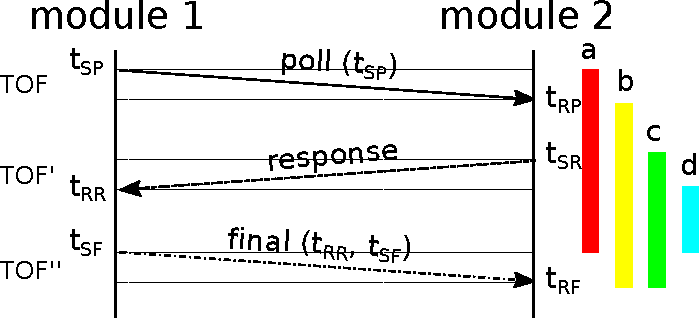
\includegraphics[width=.6\linewidth]{tex/img/bidirectional_ranging.pdf}
 \caption{Basic symmetric double-side two-way ranging packet exchange. 
 Modules 1 and 2 exchange 3 packets (\emph{poll}, \emph{response}, and \emph{final}). Module 2 then estimates the distance between the modules based on the local timestamps.}
\label{fig:bidirectional_ranging}
 \end{figure}

Module 2 can now estimate the time-of-flight and the distance between itself and module 1 based on the 6 timestampes.
The basic equations to estimate the distance between module $i$ and module $j$ (module $i$ initiates the ranging and module $j$ computes the distance) are given by:
\begin{eqnarray} %ranging between i and j (j computes distance)
a_{i} &=& t_{SF}^i-t_{SP}^i\\
b_{j,i} &=& t_{RF}^{j,i}-t_{RP}^{j,i}\\ %when j receives i
c_{j,i} &=& t_{RF}^{j,i}-t_{SR}^j\\  
d_{i,j} &=& t_{SF}^i-t_{RR}^{i,j} %i receives from j
\end{eqnarray}
\begin{eqnarray}
{TOF}_{j,i}  &\approx& \frac{1}{2}\left(c_{j,i}-d_{i,j}\frac{b_{j,i}}{a_i} \right)-\delta_{j,i}\\
\|\bm{N}_j - \bm{N}_i\| &\approx& \frac{1}{2\bm{C}}\left(c_{j,i}-d_{i,j}\frac{b_{j,i}}{a_i} \right)-o_{j,i} \label{eq:distance_estimation}\\
&\doteq& m_{j,i}-o_{j,i} .
\end{eqnarray}
The variables $a$, $b$, $c$, and $d$ are also visualized in Fig.~\ref{fig:bidirectional_ranging}.
The time-of-flight calculation between two modules $i$ and $j$ ($TOF_{j,i}=TOF_{i,j}$) is hindered by a fixed measurement offset ($\delta_{j,i}=\delta_{i,j}$).
This offset is due to antenna delays and other discrepancies  between the timestamps and actual packet reception or emission.
Whereas this offset is expected to be unique to each module, it was found that it is necessary to estimate this offset pairwise for closely located modules.
The hypothesis is that the proximity of the robot's motors and the sensor's position near the end cap's metal structure influence the antenna characteristics between pairs of modules.

Eq.~\ref{eq:distance_estimation} estimates the distances between the modules based on the time-of-flight calculation ($\bm{C}$ is the speed of light).
Rewriting the time offset $\delta_{j,i}$ as a distance offset $o_{j,i}$ (with $o_{j,i}=o_{i,j}$).
Here $\bm{N}_i$ and $\bm{N}_j$ refer to the positions of nodes $i$ and $j$ respectively (see Section~\ref{txt:ukf}).
The variables $m_{j,i}$ represent the uncorrected distance estimates.

%say offset symmetric

%lessons learned: antenna effect, bidirectional offset, restart, rx rx, 1ns pulses

The DWM1000 requires careful configuration for optimal performance.
The main configuration settings are provided in Table~\ref{tbl:dwm1000}.
The ranging modules tend to measure  non line-of-sight paths near reflective surfaces (e.g. floor, computer monitors), which may cause filter instability.
Using the DWM1000's built-in signal power estimator, such suspicious packets are rejected. 
In practice, between $30\%$ and $70\%$ of packets are rejected.

\begin{table}[h]
\centering
\caption{DWM1000 configuration}
\label{tbl:dwm1000}
\begin{tabular}{llllll}
{\bf bitrate} & {\bf channel} & {\bf preamble} &  {\bf PRF} & {\bf preamble code} \\ \hline
\SI{6.8}{\mega\bit\per\second}     & 7             & 256                    & \SI{64}{\mega\hertz}     & 17                 
\end{tabular}
\end{table}



\subsubsection{Broadcast Ranging}
Due to the large number of exchanged packets (3 per pair) bidirectional ranging between pairs of modules quickly becomes inefficient when the number of modules grows.
An alternative approach was developed using timed broadcast messages that scales linearly in the number of modules (3 packets per module).
In this setup one module periodically initiates a measurement sequence by sending out a \emph{poll} message.
When another module receives this message it emits its own \emph{poll} message after a fixed delay based on its ID, followed by \emph{response} and \emph{final} messages after additional delays.
Broadcast ranging is illustrated in Fig.~\ref{fig:broadcast_ranging}. 

\begin{figure}[tpbh]
 \centering
  \begin{turn}{270}
  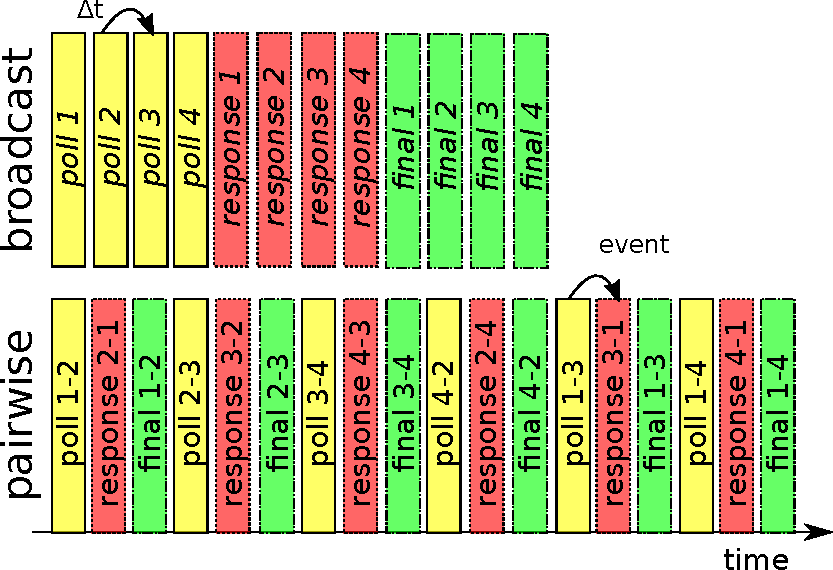
\includegraphics[width=.6\linewidth]{tex/img/broadcast_ranging.pdf}
  \end{turn}
 \caption{Packet exchange between 4 modules for bidirectional pairwise and broadcast ranging. 
 Timed broadcast messages allow for efficient ranging with a large number of modules.
  }
\label{fig:broadcast_ranging}
 \end{figure}


One disadvantage of the broadcasting approach is that the total measurement time between a pair of modules takes longer (up to \SI{60}{\milli\second} in the experimental setup)
 than a single pairwise bidirectional measurement (approx. \SI{3}{\milli\second}).
However, broadcast ranging provides two measurements for each pair of modules per measurement iteration.

Note that each module now needs to keep track of the \emph{poll} and \emph{final} packet reception times of all other modules.
The \emph{final} packet becomes longer as each module needs to transmit the \emph{response} reception time ($t_{RR}$)  of all other modules.
%The simplified packet structures are:


{%\small
%\begin{bytefield}{22}
%  \begin{rightwordgroup}{poll}{
%    \bitbox{7}{preamble} &
%    \bitbox{2}{0} &
%    \bitbox{2}{$i$} & 
%    \bitbox{3}{$t_{SP}^i$}  &
%    \bitbox{8}{checksum}
%  }\end{rightwordgroup}
%\end{bytefield}

%\begin{bytefield}{19}
%  \begin{rightwordgroup}{response}{
%    \bitbox{7}{preamble} &
%    \bitbox{2}{1} & 
%    \bitbox{2}{$i$} &  
%    \bitbox{8}{checksum}
%  }\end{rightwordgroup}
%\end{bytefield}

%\begin{bytefield}{34}
%  \begin{rightwordgroup}{final}{
%    \bitbox{7}{preamble} &
%    \bitbox{2}{2} & 
%    \bitbox{2}{$i$} &  
%    \bitbox{3}{$t_{SF}^i$} &
%    \bitbox{3}{$t_{RR}^{i,1}$}  &
%    \bitbox{3}{\ldots}  &
%    \bitbox{3}{$t_{RR}^{i,n}$}  &
%    \bitbox{8}{checksum}
%  }\end{rightwordgroup}
%\end{bytefield}
%}




\subsection{Ranging Setup}
Each end cap of SUPERball was fitted with a DWM1000 module located approximately \SI{0.1}{\metre} from the end of the strut.
To simplify the notation, the top of the MTRs (ends of the struts) and the position of the ranging sensor are assumed the same.
In practice, this offset is taken into account in the output function of the filter (see Section~\ref{txt:ukf}).

The broadcasting algorithm runs at \SI{15}{\hertz} and packet transmissions are spaced \SI{1}{\milli\second} apart.
This allows for over $20$ modules to range.
After one ranging iteration, each end cap transmits its measurements over WiFi to the ROS network. 
A ROS node then combines measurements from all MTRs, along with encoder and IMU data, into a single ROS message at  \SI{10}{\hertz}.

The fixed anchors operate in a similar way to the end caps, but are not connected to a ROS node and can not directly transmit data to the ROS network.
This means that two measurements are obtained (one in each direction) for each pair of modules on the robot, 
but only a single measurement between the fixed anchors and the modules on the robot.


\subsection{Calibration}
\label{txt:calib}
One of the design goals of this state estimation method is quick deployment in new environments without significant manual calibration.
To achieve this, an automatic calibration procedure was implemented to jointly estimate the constellation of fixed modules (anchors, defining an external reference frame) 
and the pairwise sensor offsets ($o_{i,j}$).
Calibration is performed - similar to common motion capture systems - by moving the robot around, while recording the uncorrected distance measurements ($m_{j,i}$).

After recording a dataset, reconstruction error is minimized $L$ by optimizing over the offsets $\bm{o}$ ($o_{i,j}$ rearranged as a vector), the estimated anchor locations $\bm{N}^{est}$, and the estimated moving module locations $\bm{N}^{float}[1\ldots n_{samples}]$ (i.e. the module on the robot's end caps):
\begin{align}
\resizebox{.91\hsize}{!}{$L\left(i,j,t\right) = \left( \|\bm{N}^{anchor}_i - \bm{N}^{float}_{j}\left[t\right]\|-o_{j,i} - m_{i,j}\left[t\right] \right)^2$ \label{eq:l_single}}\\
\resizebox{.91\hsize}{!}{$L\left(\bm{o},\bm{N}^{anchor},\bm{N}^{float}[1\ldots n_{samples}]\right) = \sum_{i,j,t}\alpha_{j,t}L\left(i,j,t\right)$. \label{eq:l_full}}
\end{align}

The brackets in $\bm{N}^{float}[1\ldots n_{samples}]$ indicate the moving module locations (MTR positions) at a specific timestep. 
For example $\bm{N}^{float}[5]$ contains the estimated end cap positions at timestep 5 in the recorded dataset.
In Eq.~\ref{eq:l_full}, $i$ iterates over anchors, $j$ iterates over moving nodes and $t$ iterates over samples.
The indicator variables $\alpha_{j,t}$ are equal to $1$ when for sample $t$ there are at least $4$ valid measurements to the fixed module for moving module $j$ (i.e. the number of DOFs reduces).

In practice, constraints are added on the bar lengths, which take the same form as Eq.~\ref{eq:l_single} with the offsets set to $0$.
BFGS~\cite{battiti1990bfgs} is used to minimize Eq.~\ref{eq:l_full} with  a dataset containing approximately $400$ timesteps selected randomly from a few minutes of movement of the robot.
Although the algorithm works without prior knowledge, providing the relative positions of $3$ fixed nodes ($3$ manual measurements) significantly improves the success rate as there are no guarantees on global convergence.

Once the external offsets (between the anchors and moving nodes) and the module positions are known, the offsets can be estimated between moving nodes in a straightforward way by computing the difference between the estimated internal distances and the uncorrected distance measurements.


%%%%%%%%%%%%%%%%%%%%%%%%%%%%%%%%%%%%%%%%%%%%%%%%%%%%%%%%%%%%%%%%%%%%%%%%%%%%%%%%


\section{Filter Design}
\label{txt:ukf}

Tensegrity systems are nonlinear and exhibit hybrid dynamics due to cable slack conditions and  interactions with the environment that involve collision and friction. This warrants a robust filter design to track the robot's behavior.

The commonly used Extended Kalman Filter (EKF) does not perform well on highly nonlinear systems where first-order approximations offer poor representations of the propagation of uncertainties.
Additionally the EKF requires computation of time-derivatives through system dynamics and output functions which is challenging for a model with complex hybrid dynamics. 

The sigma point Unscented Kalman Filter (UKF) does not require derivatives through the system dynamics and is third order accurate when propagating Gaussian Random Variables through nonlinear dynamics~\cite{wan2000unscented}. The computational cost of the UKF is comparable to that of the EKF, but for tensegrity systems which commonly have a large range of stiffnesses and a high number of state variables the time-update of the sigma points dominates computational cost. As such, the methods used to reduce computational cost of dynamic simulation will be described, then in the following section the outline of the specific UKF implementation for the \SB{} prototype.

\subsection{Dynamic Modelling} 
\label{sec:dynamic_modeling_sb}

The UKF requires a dynamic model which balances model fidelity and computational efficiency since it requires a large number of simulations to be run in parallel. 
The model implemented for the tensegrity system is a spring-mass net and the following incomplete list of simplifying assumptions where used:
\begin{itemize}
  \item Only point masses located at each node point
  \item All internal and external forces are applied at nodes
  \item Members exert only linear stiffness and damping
  \item Unilateral forcing in cables
  \item Flat ground at a known height with Coulomb friction
  \item No bar or string collision modelling
\end{itemize}
%This is a common approach for modeling tensegrity systems, and force density approaches for this problem are described in \textcolor{red}{cite}. Below we describe some careful manipulation of the equations within this force density framework which allowed us to run the parallel simulations while leaving computational bandwidth for other requisite operations such as communication and data visualization. 

For a tensegrity with $n$ nodes and $m$ members, the member force densities, 
$\boldsymbol{q}\in\mathbb{R}^{m}$, can be transformed into nodal forces,
$\boldsymbol{F_m}\in\mathbb{R}^{n\times 3}$, by using the current Cartesian nodal positions,
$\boldsymbol{N}\in\mathbb{R}^{n\times 3}$, and the connectivity matrix,
$\boldsymbol{C}\in\mathbb{R}^{m\times n}$, as described in \cite{skelton2009tensegrity}. This operation is described by the equation:
$$
\boldsymbol{F_m} = \boldsymbol{C}^{T} diag(\boldsymbol{q}) \boldsymbol{C} \boldsymbol{N},
$$
where $diag(\cdot)$ represents the creation of a diagonal matrix with the vector argument along its main diagonal.
First, note that $\boldsymbol{C} \boldsymbol{N}$ produces a matrix $\boldsymbol{U}\in\mathbb{R}^{m\times 3}$ where each row corresponds to a vector that points between the $i$th and $j$th nodes spanned by each member. 
Therefore, this first matrix multiplication can be replaced with vector indexing as $\boldsymbol{U}_{k} = \boldsymbol{N}_{i} - \boldsymbol{N}_{j}$,
where the notation $\boldsymbol{U}_{k}$ is used to denote the $k$th row of matrix $\boldsymbol{U}$. If one then computes $\boldsymbol{V}=\boldsymbol{C}\frac{d\boldsymbol{N}}{dt}$ with the same method
%%%% NOTE This was the old sentence, but X_{l} didn't make sense... So I assumed it was suppose to be U_{k}. Is that correct?
%where we use the notation $\boldsymbol{X}_{l}$ to denote the $l$th row of matrix $\boldsymbol{X}$. If we then compute $\boldsymbol{V}=\boldsymbol{C}\frac{d\boldsymbol{N}}{dt}$ with the same method 
as $\boldsymbol{U}$, one would obtain a matrix of relative member velocities.
The matrices $\boldsymbol{U}$ and $\boldsymbol{V}$ are used to calculate member lengths as $L_k = |\boldsymbol{U}_k|_2$ and member velocities as $\frac{d}{dt}(L_k) = \frac{\boldsymbol{U}_k(\boldsymbol{V}_k)^T}{L_k}.$

Member force densities, $\boldsymbol{q}$, are then calculated using Hooke's law and viscous damping as:
$$
\boldsymbol{q}_k = K_k(1 - \frac{L_{0k}}{L_k}) - \frac{c_k}{L_k} \frac{d}{dt}(L_k).
$$
Here $K_k$ and $c_k$ denote the $k$th member's stiffness and damping constants, respectively.
Note that cables require some additional case handling to ensure unilateral forcing.

Scaling each $\boldsymbol{U}_k$ by $\boldsymbol{q}_k$ yields a matrix whose rows correspond to vector forces of the members. 
Denote this matrix as $\boldsymbol{U}^q\in\mathbb{R}^{m\times 3}$, and note that $\boldsymbol{U}^q = diag(\boldsymbol{q}) \boldsymbol{C} \boldsymbol{N}$.
Thus this matrix of member forces can be easily applied to the nodes using:
$$
\boldsymbol{F_m} = \boldsymbol{C}^{T} \boldsymbol{U}^q.
$$
A method for computing nodal forces exerted by the members is now obtained, and only ground interaction forces need to be computed, which will be denote as $\boldsymbol{F}_g$.
Ground interaction forces were computed using the numerical approach in~\cite{yamane2006stable}. The nodal accelerations can then be written as:
$$
\frac{d^2\boldsymbol{N}}{dt^2} = \boldsymbol{M}^{-1}(\boldsymbol{F}_m+ \boldsymbol{F}_g) -  \boldsymbol{G},
$$
where $\boldsymbol{M}\in\mathbb{R}^{n\times n}$ is a diagonal matrix whose diagonal entries are the masses of each node and $\boldsymbol{G}\in\mathbb{R}^{n\times 3}$ is matrix with identical rows equal to the vector acceleration due to gravity. 
It is then straightforward to simulate this second order ODE using traditional numerical methods. 

Note also that it is possible to propagate many parallel simulations efficiently by concatenating multiple $\boldsymbol{N}$ matrices column wise to produce  $\boldsymbol{N}_{\parallel}\in\mathbb{R}^{n\times 3l}$ for $l$ parallel simulations.
The resultant vectorization of many of the operations yields significant gains in computational speed with some careful handling of matrix dimensions.   

\subsection{UKF Implementation}

A traditional UKF was implemented as outlined in \cite{wan2000unscented} with additive Gaussian noise for state variables and measurements.

Several parameters are defined for tuning the behavior of the UKF, namely $\alpha$, $\beta$ and $\kappa$, where $\alpha$ determines the spread of the sigma points generated by the unscented transformation, $\beta$ is used to incorporate prior knowledge of distribution, and $\kappa$ is a secondary scaling parameter.
Hand tuning obtained these parameters to the values $\alpha = 0.0139$, $\beta = 2$ for Gaussian distributions and $\kappa = 0$ and found this to yield an adequately stable filter.

Defining state variables as $\boldsymbol{N}$ and $\frac{d\boldsymbol{N}}{dt}$ stacked in a vector $\boldsymbol{y}\in\mathbb{R}^{L}$ where $L = 6n$ is the number of state variables. 
Also, independent state noise is assumed with variance $\lambda_y = 0.4$ thus with covariance $\boldsymbol{R} = \lambda_y\bm{I}_L$.

\begin{figure}[tpbh]
 \centering
  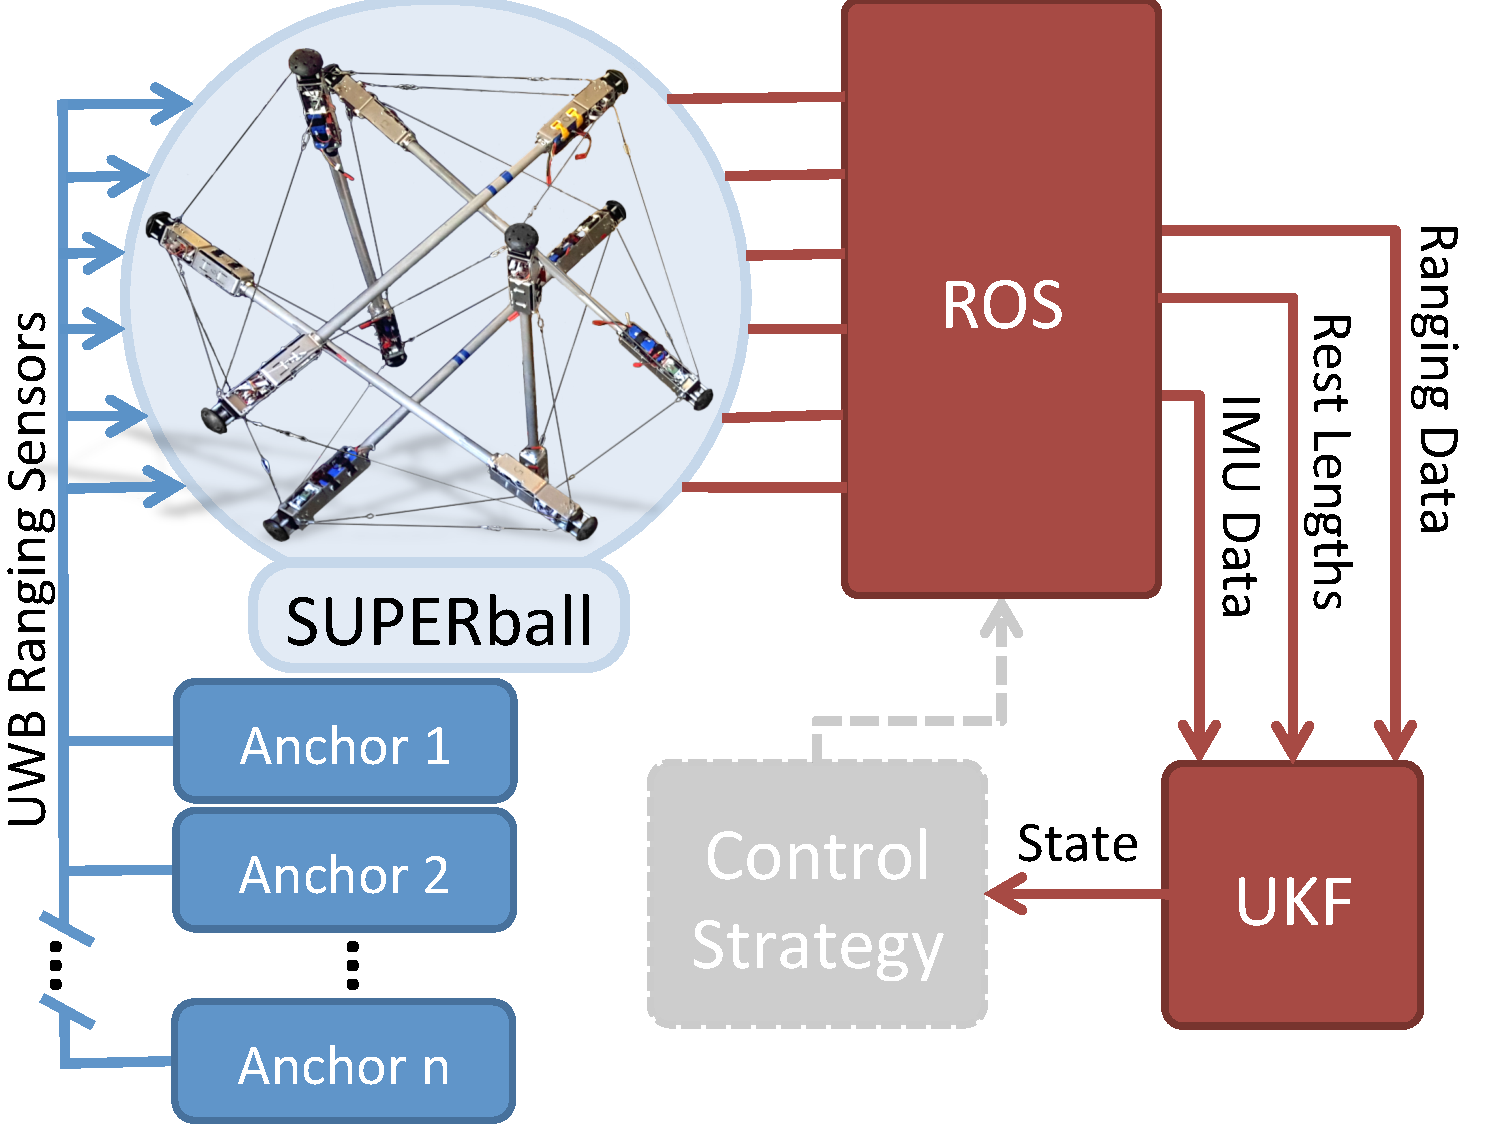
\includegraphics[width=0.7\linewidth]{tex/img/flow_chartSB.pdf}
 \caption{Block diagram of data flow within the system. Red signals are passed as ROS messages and blue signals are passed using the ranging modules. Note that each rod contains two ranging sensors located at each end of the rod. The gray control strategy block represents a to-be-designed state-feedback control strategy.}
\label{fig:UKFflowChart}
 \end{figure}

%For measurements we take the minimum angle between each bar vector and the z-axis, $\theta\in\mathbb{R}^{b}$ where $b$ is the number of bar angles available at the given time step and all ranging measures, $\boldsymbol{r}\in\mathbb{R}^{a}$, where $a$ is the number of ranging measures available at a given time step.
The measurement data used is estimated orientation data from the robot's IMUs using a gradient descent AHRS algorithm based on~\cite{madgwick2011estimation}, $\theta\in\mathbb{R}^{b}$ where $b$ is the number of bar angles available at the given time step and all ranging measures, $\boldsymbol{r}\in\mathbb{R}^{a}$, where $a$ is the number of ranging measures available at a given time step.
Independent noise is again assumed and represented by $\lambda_\theta$ and $\lambda_r$. 
The measurement covariance matrix is then defined as:
$$
\boldsymbol{Q} =  \left[ \begin{array}{ccc} \lambda_\theta\bm{I}_b & \boldsymbol{0} \\
                         \boldsymbol{0}        & \lambda_r\bm{I}_a  \end{array} \right].
$$
These user defined variables are then used within the framework of the UKF to forward propagate both the current expected value of the state as well as its covariance. 
Fig.~\ref{fig:UKFflowChart} shows an overview of the complete state estimation setup. 

\section{Filter Evaluation}
\subsection{Experimental Setup}
To evaluate the performance of the UKF, eight "fixed anchor" ranging base stations are used and calibrated as detailed in Section~\ref{txt:calib}.
Each end cap of \SB{} was then able to get a distance measurement to each base station.
This information was sent over ROS along with IMU data (yaw,pitch,roll) and cable rest lengths to the UKF.
The base stations were placed in a pattern to cover an area of approximately \SI{91}{\meter^2}. 
Each base station's relative location to each other may be seen in Fig.~\ref{fig:SUPERballMATLAB}.
\SB{} and the base stations were then used to show the UKF tracking a local trajectory of end caps and a global trajectory of the robotic system.
In each of these experiments, the UKF was allowed time to settle from initial conditions upon starting the filter.
This ensured that any erroneous states due to poor initial conditioning did not affect the filter's overall performance. 

\begin{figure}[tpbh]
 \centering
  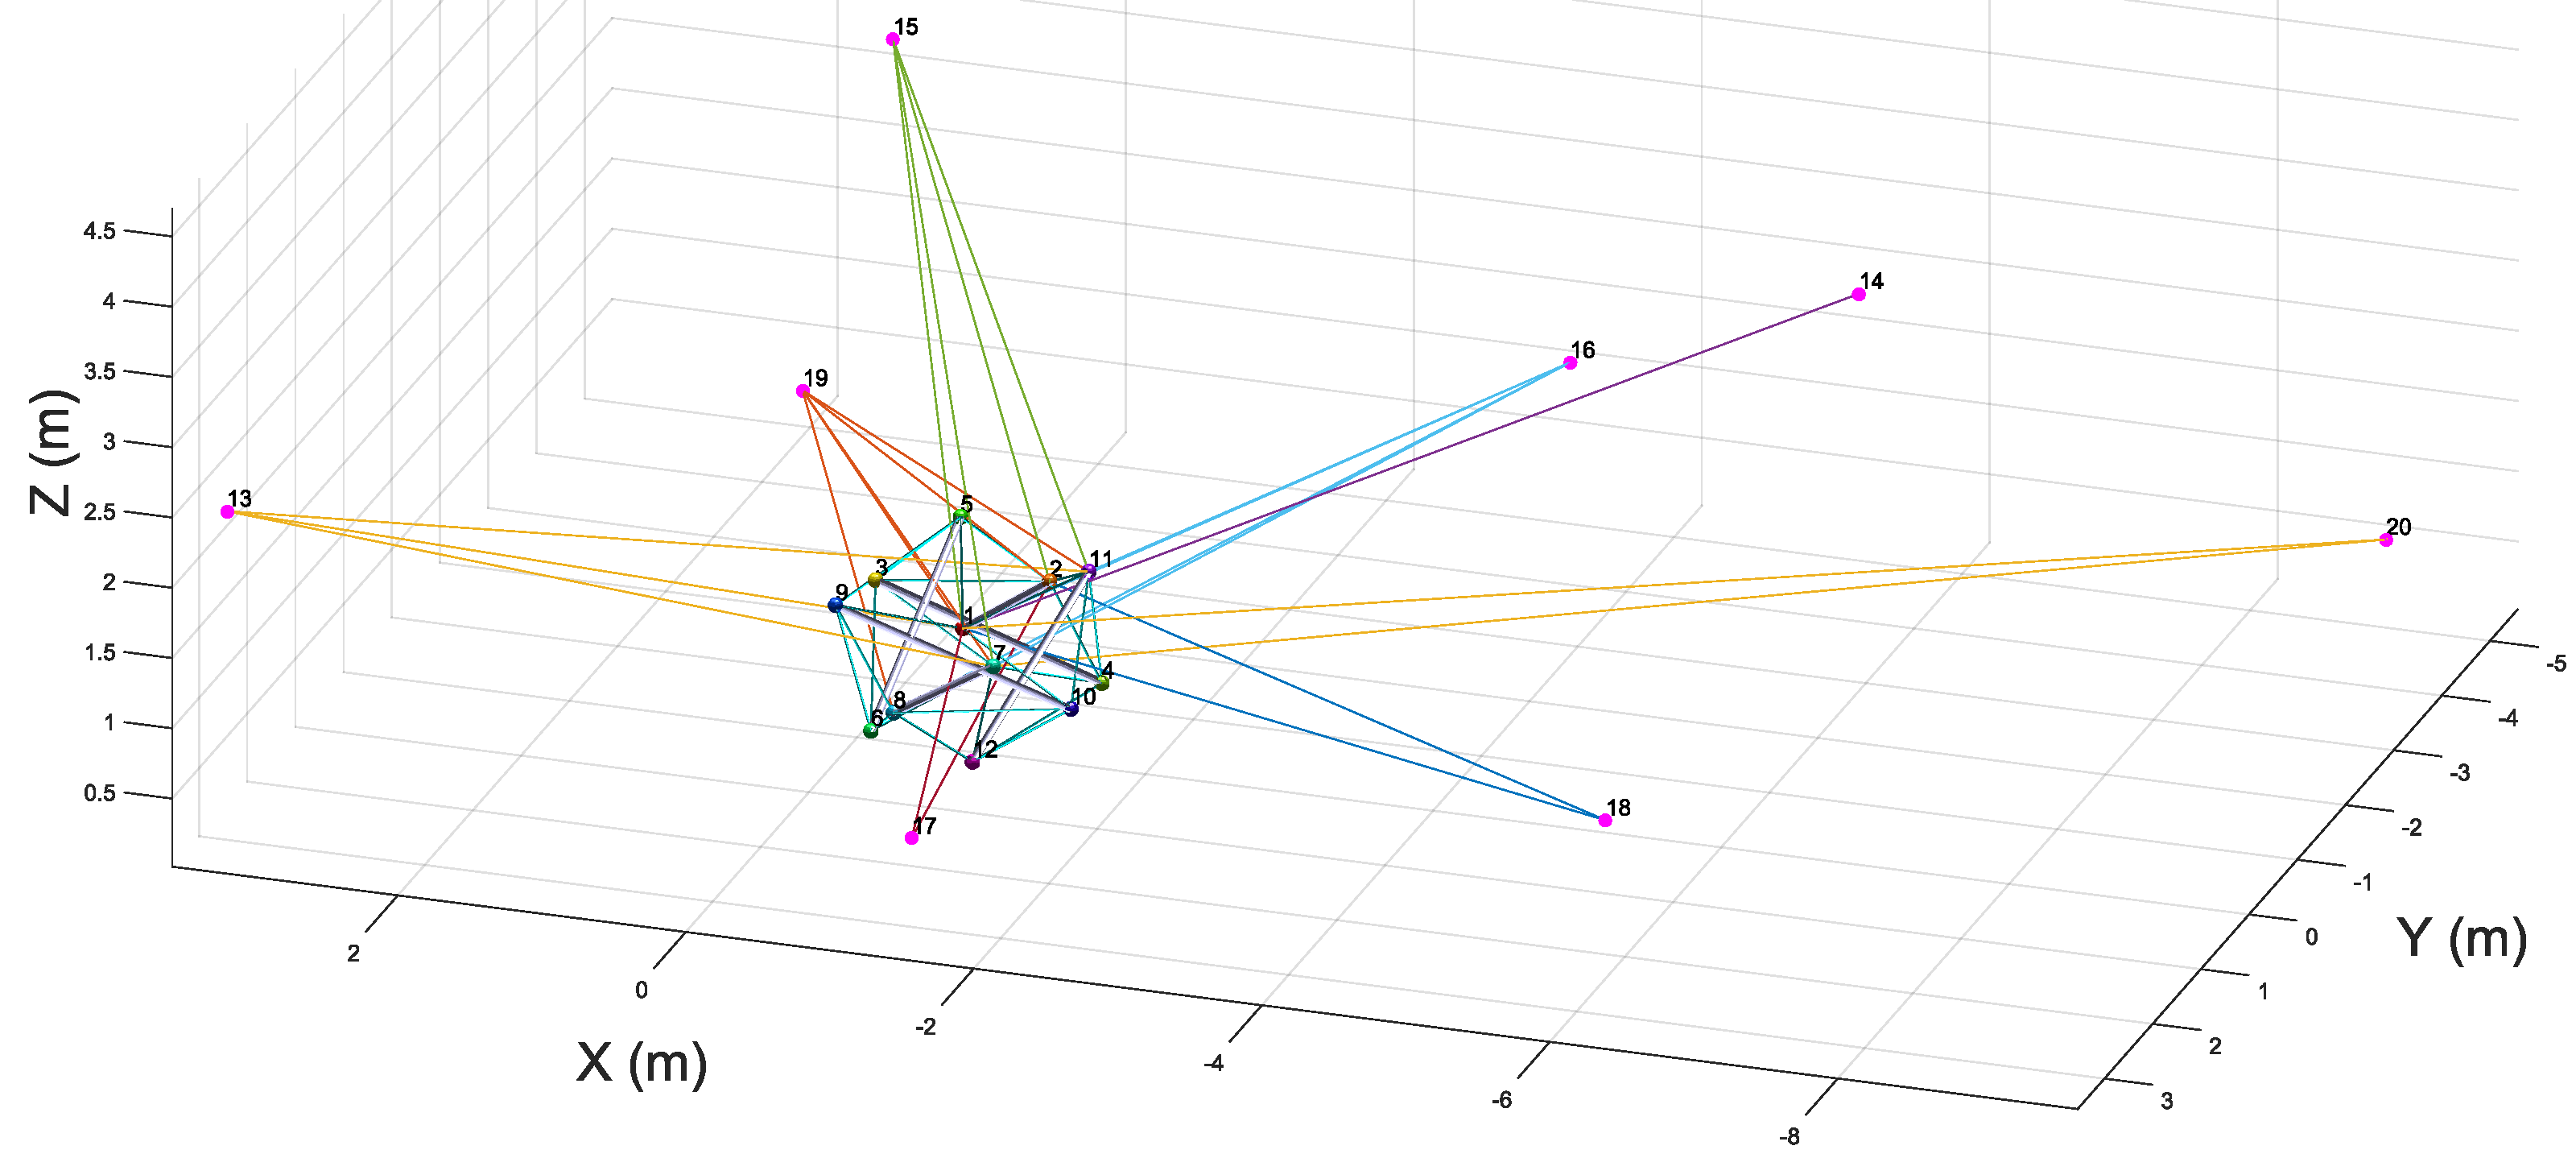
\includegraphics[width=\linewidth]{tex/img/matlab_figure_ranging_b45.pdf}
 \caption{Visualization of the UKF output. \SB{} sits in the middle of the plot surrounded by 8 ranging base stations. Lines between the robot and the base stations indicate valid ranging measures during this timestep.}
\label{fig:SUPERballMATLAB}
 \end{figure}

\subsection{Local Trajectory Tracking}
In order to track a local trajectory, \SB{} remained stationary while two of its actuators tracked phase shifted stepwise sinusoidal patterns.
During the period of actuation, two end cap trajectories were tracked on \SB{} and compared to the trajectory outputs of the UKF.
One end cap was directly connected to an actuated cable (end cap 2), while the other end cap had no actuated cables affixed to it (end cap 1).
To obtain a ground truth for the position trajectory, a camera that measured the position of each end cap was positioned next to the robot.
Both end caps started at the same relative height and the majority of movement of both fell within the plane parallel to the camera.
Fig.~\ref{fig:smalldisplacement} shows the measured and UKF global positions of the two end caps through time.

\begin{figure}[tpbh]
  \centering
  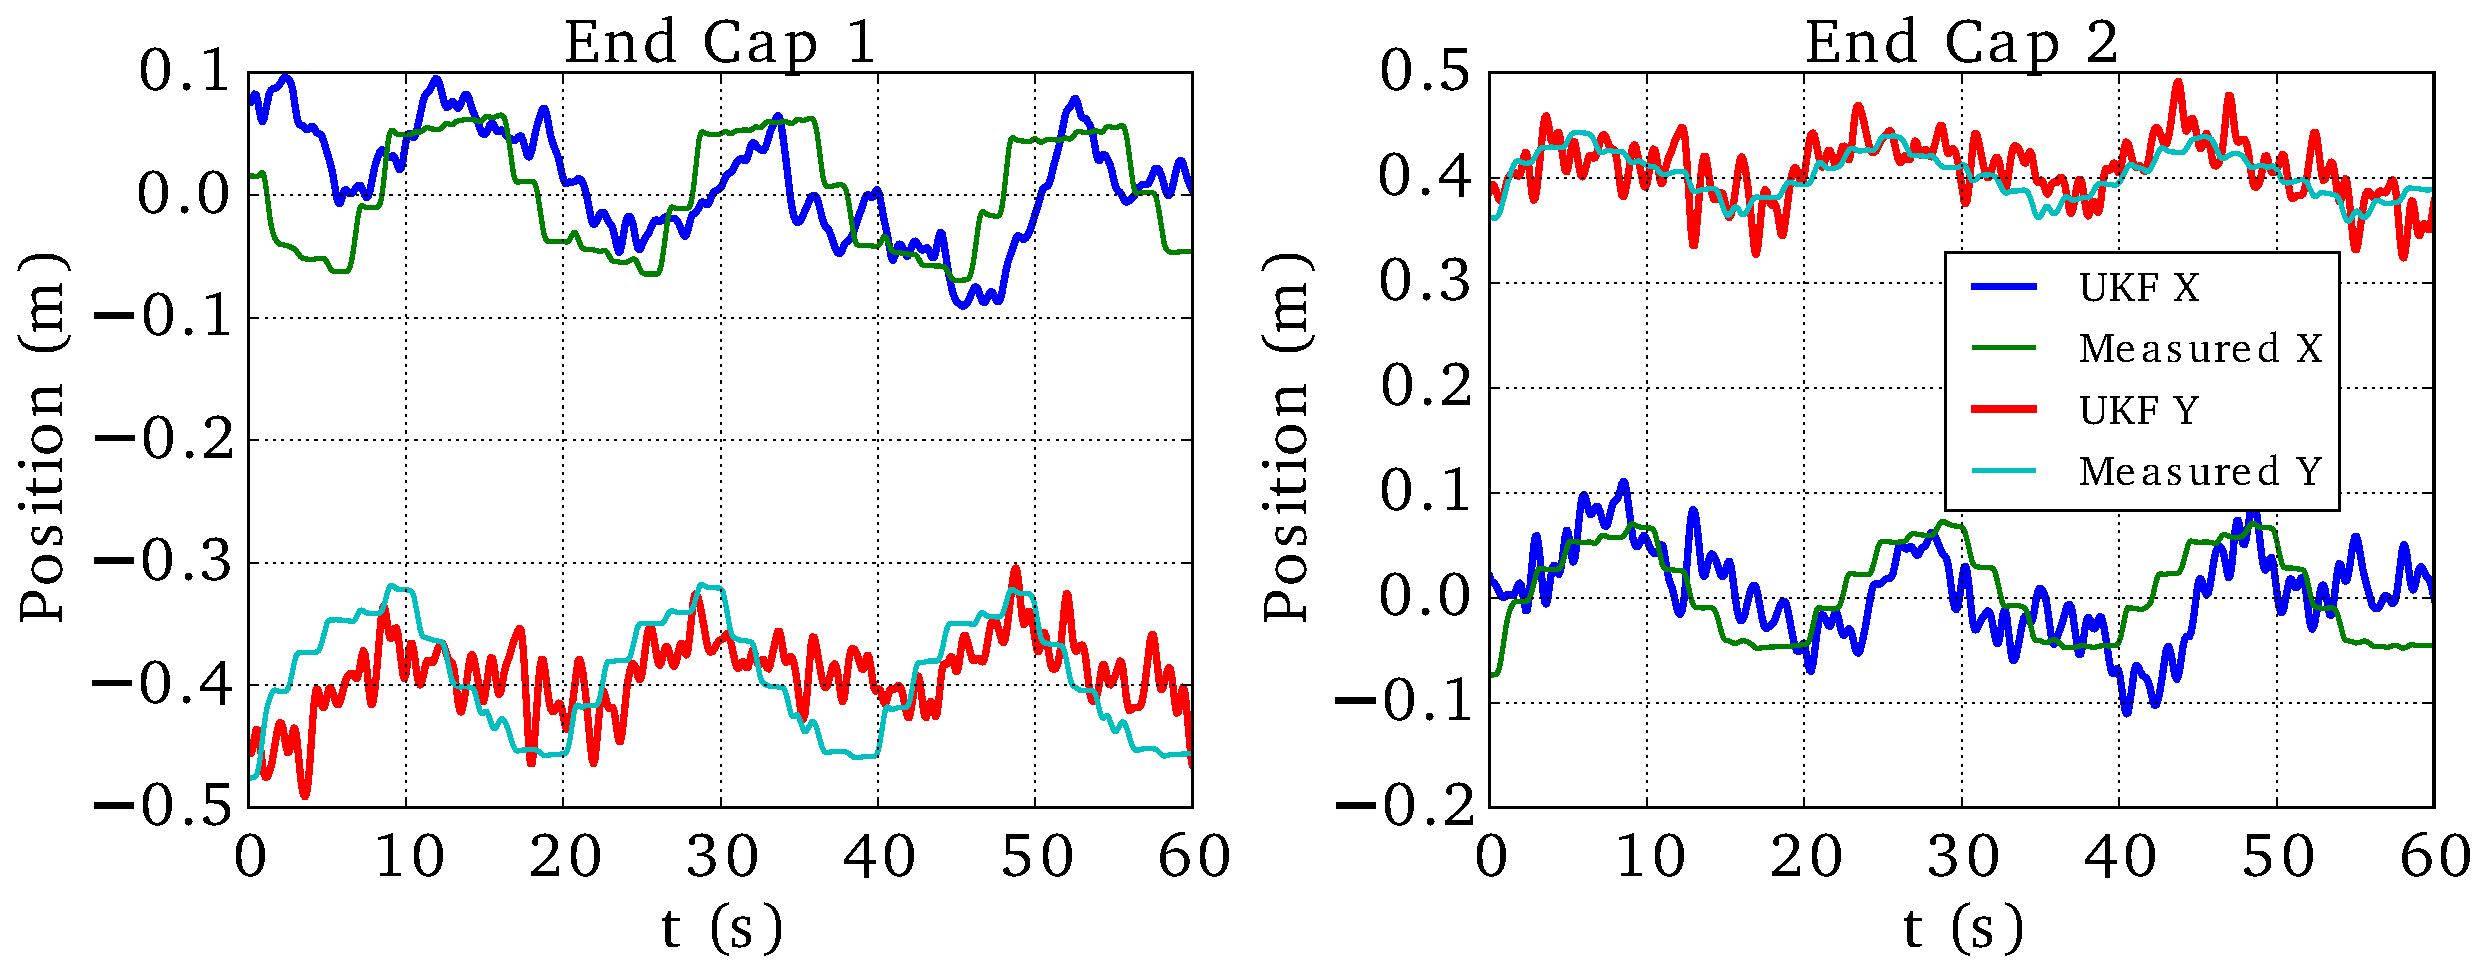
\includegraphics[width=1\linewidth]{tex/img/Node_tracking_1-11.pdf}
  \caption{Position plotted through time for both end cap 1 and end cap 2. The thin line represents the position output measured by the camera tracking system, and the bold line represents the position output from the UKF filter. As expected, there is a time domain lag between the measured and estimated positions.}
  \label{fig:smalldisplacement}
\end{figure}


% For this experiment, the cables between end caps 1 and 11 and end caps 12 and 8 were actuated.
% The UKF is able to track the end cap movements quite well with some displacement error in the Y position for end cap 1.
% Upon further inspection of the input data to the UKF, there was a high packet loss between end cap 1 and the base stations. 
% This coupled with a mismatched base model, might be the cause for this error.

\subsection{Global Trajectory Tracking}
For global trajectory tracking, \SB{} was actuated to induce a transition from one base triangle rolling through to another base triangle as presented in \cite{sabelhaus2015system}.
%The state of \SB{} was tracked using the UKF.
Ground truth for this experiment was ascertained by marking and measuring the positions of each base triangle's end caps before and after a face transition.
%Fig.~\ref{fig:3roll_perspective} shows a 3D plot of the UKF generated states for the beginning and end of the experiment.
%Each colored triangle represents a base triangle and the robot implements two full transitions starting from the red triangle and ending on the blue.
4 settings of the state estimator were evaluated. \emph{Full}: The state estimator as described in Section~\ref{txt:ukf} with all IMU and ranging sensors. \emph{no IMU}: Only the ranging sensors are enabled. \emph{full w. cst. offset}: Same as \emph{full}, but the offsets $\bm{o}$ are set to a constant instead of optimized individually. \emph{4 base station ranging sensors}: 50\% of the base station ranging sensors are disabled. 
The results of this experiment are presented in Fig.~\ref{fig:3roll_triangles}~and~\ref{fig:3roll_xz_position}.
\begin{figure}[tpbh]
 \centering
  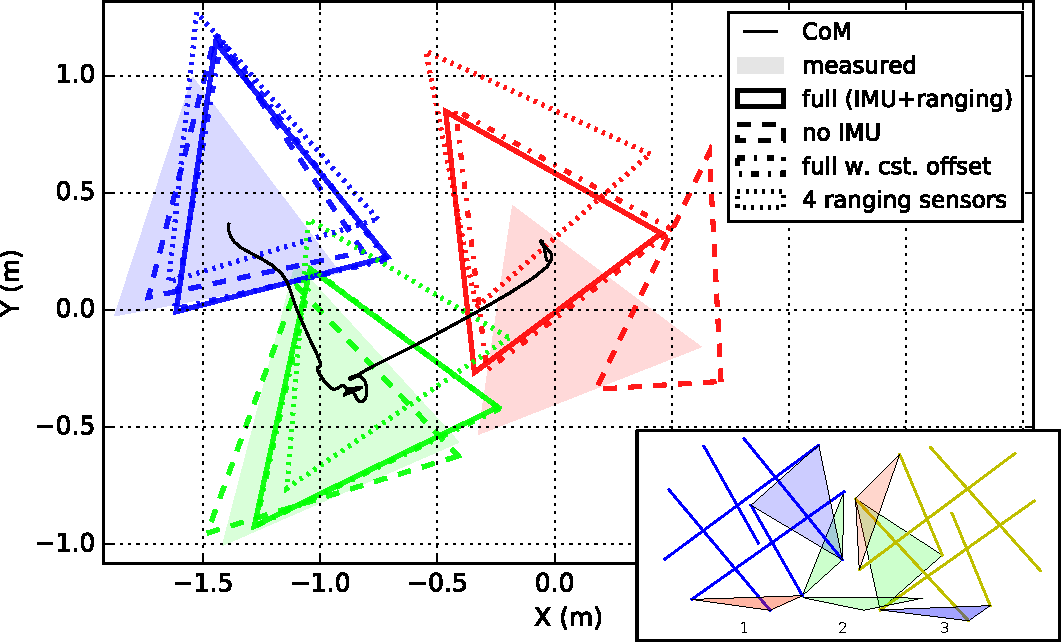
\includegraphics[width=\linewidth]{tex/img/top_view.pdf}
\caption{Top down view of the triangular faces to which the robot transitions during the global trajectory tracking experiment for various setting of the state estimator. The small inset illustrates the movement of the robot. The line shows the estimated center of mass (CoM) using the \emph{full} settings.
Finding the initial position (origin) is hard for all settings, and without the IMUs the estimator does not find the correct initial face.
After a first roll, tracking becomes more accurate. The offsets $\bm{o}$ have a minimal impact, which indicates that the calibration routine is sufficiently accurate.   }
\label{fig:3roll_triangles}
 \end{figure}
\begin{figure}[tpbh]
  \centering
  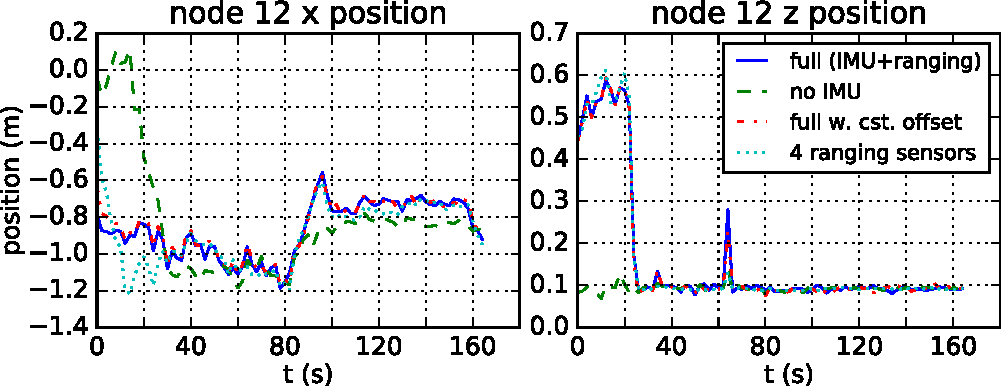
\includegraphics[width=\linewidth]{tex/img/roll_x_z_zoom.pdf}
\caption{X and Y position of end cap 12 as a function of time for the various estimator settings. The end cap was initially off the ground and touches the ground after the first roll. This is not tracked correctly when the IMUs are disabled. The system works as expected when 4 base stations ranging sensors are disabled, but with slower convergence and more noise on the robot's position. Around \SI{60}{s} there's a spurious IMU value from which  the state estimator recovers. 
}
  \label{fig:3roll_xz_position}
\end{figure}
\chapter{Control for \SB{} Locomotion}
\label{controls}

\section{Basic Locomotion Concepts for a Icosahedron Tensegrity Robot}
\label{basic_locomotion}

Locomotion for tensegrity structures like \SB{} is achieved by deforming the structure in a way in which moves the system's center of mass to an unstable configuration, tipping the robot over.
This deformation is usually achieved by either changing the length of the main cable network on the outside of the robot~\cite{sabelhaus2015system,kim2014rapid} or by adding additional cables which run through the structure connecting non-parallel rods~\cite{caluwaerts2014design}.
For the rest of this section, deformation is assumed to be done by actuating the main cable network on the outside of the robot since this is how \SB{} is deformed.

% \SB{} is a tensegrity structure is the shape of an icosahedron.
An regular convex icosahedron is a geometric shape consisting of eight equilateral triangle interlaced with twelve isosceles triangles.
In a passively sable configuration, the bottom of an icosahedron will be resting on either an equilateral or a isosceles triangle.
Utilizing this knowledge, the most simple method for moving the center of mass of an icosahedron can be obtained by changing the length of one side of the bottom triangle to near zero.
This will always move the center of mass to an unstable configuration by effectively reducing the bottom triangle, as seen if figure~\ref{fig:single_flop}, which will cause the robot to transition to another face.
However, this simple control method is not always obtainable on a real robotic system due to limitation on actuation or design methodology.
For \SB{}, this control method is obtainable when the system only has the battery mounted required to actuate the single motor reducing the overall system weight.
Figure~\ref{fig:superball_flop_flat} shows this single motor face transition on a weight reduced \SB{}.

\begin{figure}[thpb]
      \centering
      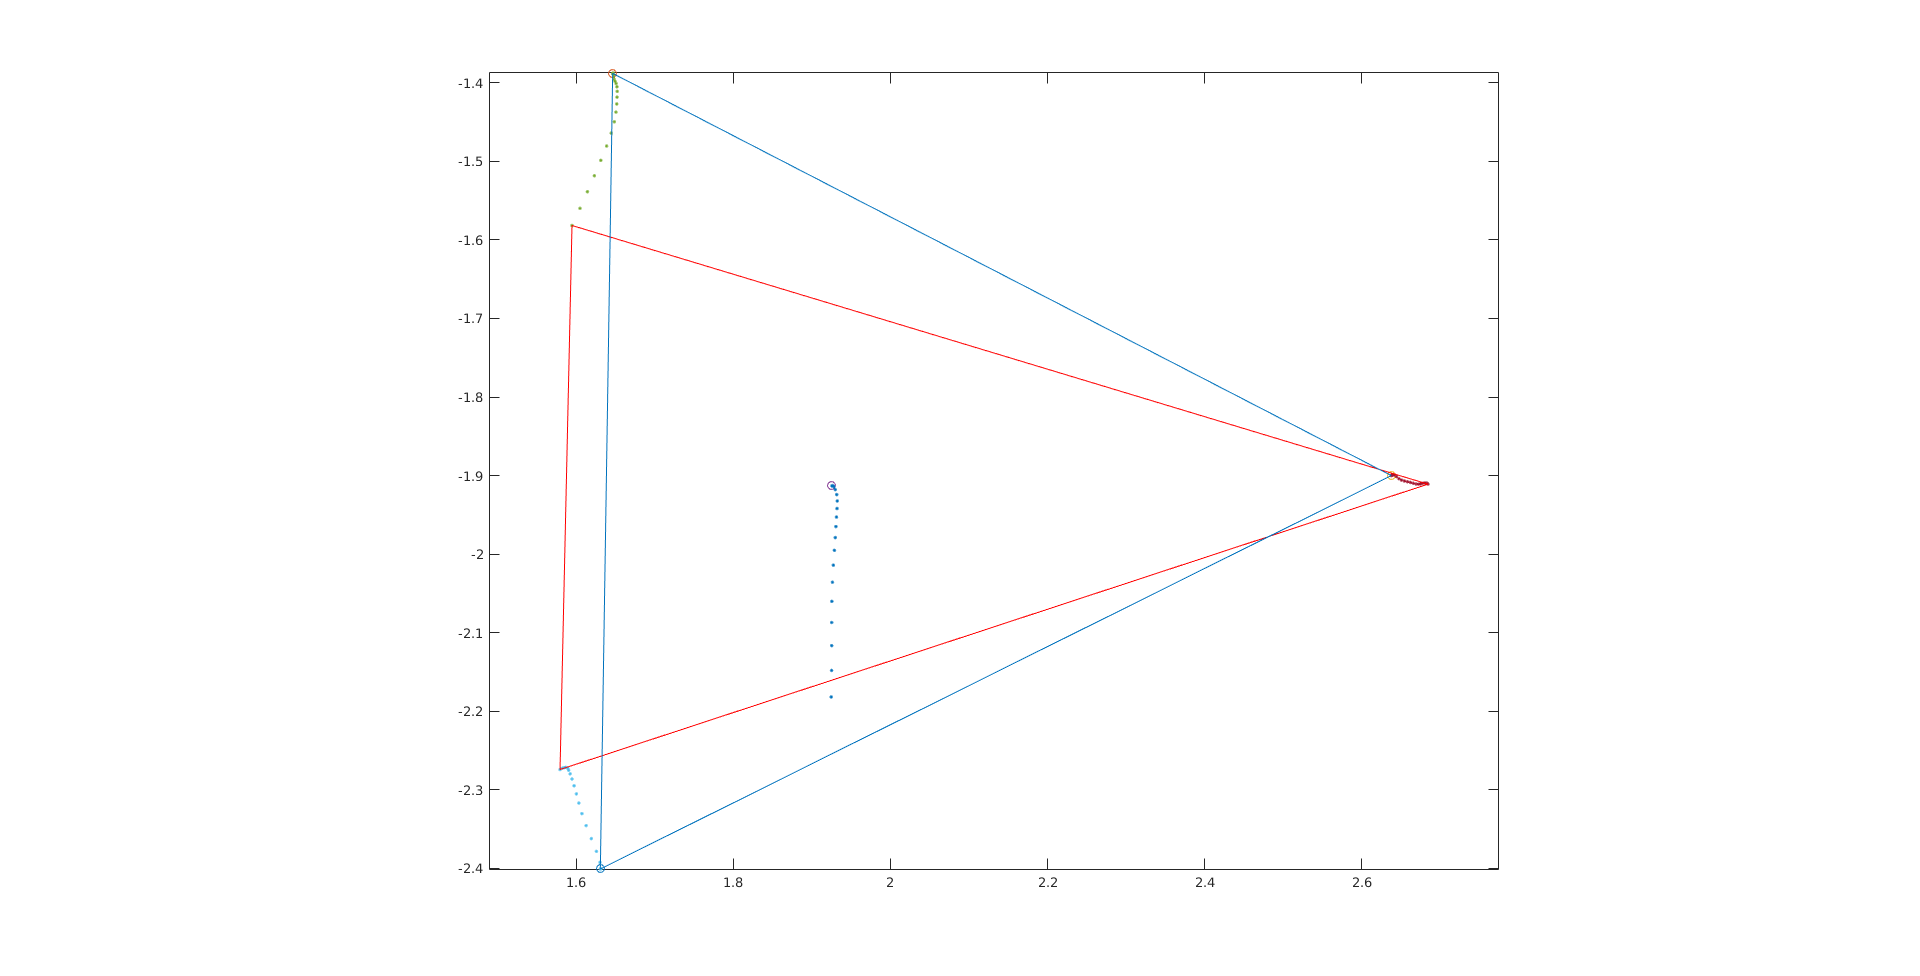
\includegraphics[width=0.8\columnwidth]{tex/img/Single_flop_bottom_triangle}
      \caption{This is XY data of the bottom triangle of a NTRT simulation of \SB{} performing a single face transition by changing only one side of the bottom triangle.
      No other cable on the system is being actuated during this simulation.
      The red triangle is the bottom triangle at the start of the simulation. 
      The centralized circle represents the center of mass (CoM) of the entire simulated \SB{}. 
      The blue triangle is the configuration where the CoM moves out of the bottom triangle and the robot begins to transition to another face.
      Thus, under ideal conditions and actuation limits, a \SB{} like structure can perform a face transition by the changing of a single cable.}
      \label{fig:single_flop}
\end{figure}

\begin{figure}[thbp]
    \centering
    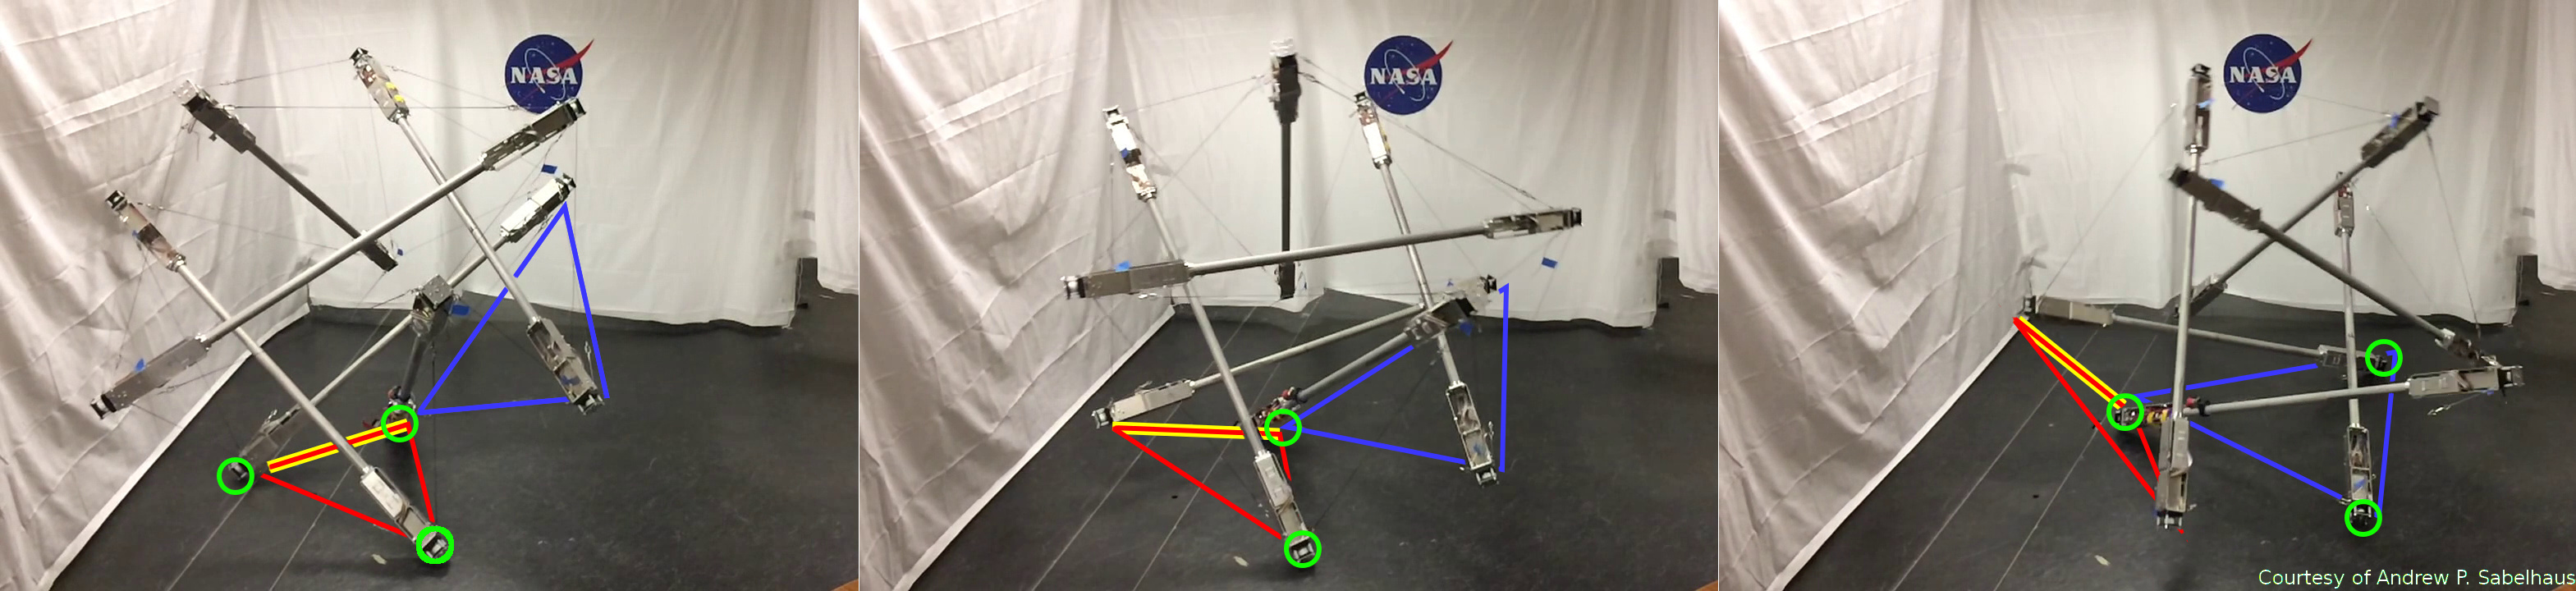
\includegraphics[width=1\linewidth]{tex/img/superball_flop_combined_betterlabels}
    \caption{\SB{} performing a single face-change movement, from one equilateral triangular face to another. The robot begins with all MTRs of the red triangle touching the ground. Then, \SB{} retracts the yellow-highlighted cable on the red triangle, inducing movement. Frame 2 shows \SB{} halfway through the movement with only two points of contact on the ground. Finally, frame 3 shows \SB{} at the end, with all 3 points of the blue triangle in ground contact.}
    \label{fig:superball_flop_flat}
\end{figure}

\SB{} is an underactuated icosahedron tensegrity robot.
Of the 24 connection cables, \SB{} only has 12 cables which are actively actuated and the other cables are passive as discussed in section~\ref{design}.
Since each MTR is manufactured with the same elements, each of the four cables attached to it are one of four types: an actuated cable attached to a motor, an actuated cable from an adjacent MTR terminating at this MTR, a passive cable attached to a spring, or a passive cable from an adjacent MTR terminating at this MTR.
Therefore, there is a unique pattern of cables, and care is needed when choosing this pattern for locomotion. 

For \SB{}, a symmetric pattern is used where each equilateral triangle has at least one actuator associated with one of its sides.
As stated in section~\ref{design}, \SB{} has eight equilateral triangles, so at most three triangles will have more than one actuated side.
These triangles are evenly spaced round the surface of the robot such that there are "rings" of six equilateral triangles with the other two triangles flanking this ring.
Forward locomotion is then achieved by transitioning the structure such that each of the six equilateral triangles on this "ring" come in complete contact with the ground at some instantaneous point in time.
Since a symmetric pattern was desired, it was chosen to placing one actuator per "ring" triangle in such a way where the theoretical full acutation length change of that triangle side would cause the robot to transition towards the next sequential equilateral triangle on that "ring".
The other six motors where then attached as all the side of the remaining two equilateral triangles, those not associated with the "ring".
Figure~\ref{fig:actuator_pattern} (a) shows a graphical overlay of the actuation "ring" and the fully actuated triangles marked in red and blue, respectively.
Figure~\ref{fig:actuator_pattern} (b) is a icosahedron rolled out to show the "walking" gait pattern achieved by rolling about the actuation "ring".

\begin{figure}[thbp]
    \centering
    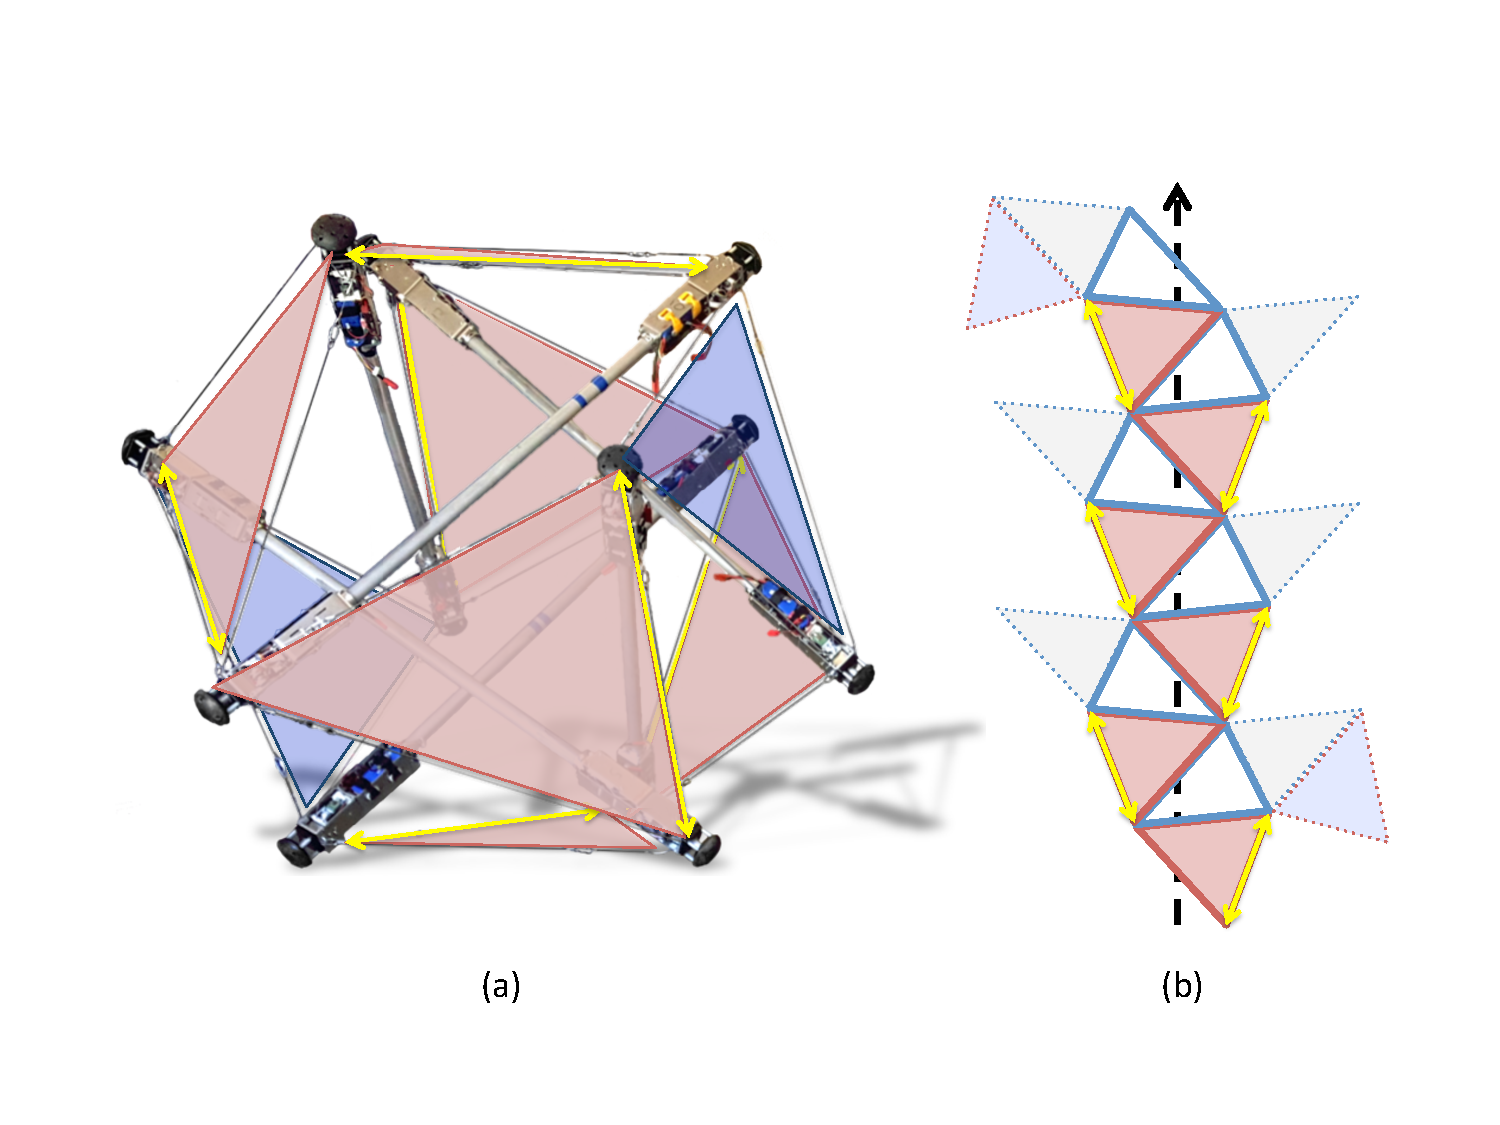
\includegraphics[width=0.6\linewidth]{tex/img/SB_RedvBlue_with_Walk}
    \caption{This image shows the actuation pattern used on \SB{}. There are 8 equilateral triangles, shown in either red or blue. Each red triangle represents a face with only one of the three cable sides actuated. These actuated cables are noted by the yellow double arrows. Each blue triangle, which are not  has actuators on all three cable sides. The basic forward rolling of \SB{} has the robot landing with a red triangle fully on the ground during locomotion. Blue triangles don't touch the ground during this forward rolling pattern. Figure (a) shows each triangle highlighted on \SB{} and figure (b) shows the forward locomotion pattern, or walking pattern, of \SB{}.}
    \label{fig:actuator_pattern}
\end{figure}


% There has been many open loop control techniques that explored this concept through the use of form finding static poses~\cite{}\textcolor{red}{bliss, mirats-tur}.
% Their simulation results show some very promising results for locomotion of variou
% xKim et al~\cite{kim2015robust} developed a method which address some of these issues, but requires .... \textcolor{red}{something non-ideal}.
% However, these techniques do not generalize well to ill-formed robot parameters between simulation and a physical robot, and usually constrain the search space to small manifolds for valid structure configurations.
% When the manifolds are expanded, the search space can become very large resulting in slow results that require a large number of 

% \textcolor{blue}{write about Atil's work and Brian's.}


%Another interesting point could be made about there being two classes of tensegrity robots.  Many of the early approaches stemmed directly out of the modeling and mathematics of static tensegrity structures, which used low-creep cables for stability, and such designs result in very small manifolds of valid structures, with many of the changes in cables lengths resulting in the robot becoming unstable and collapsing as there was no valid equilibrium pose.

\section{Hand-Tuned Stepwise Controller}
\label{hand_stepwise}
The initial controller developed for \SB{} was a basic open loop, hand tuned controller.
Motor position commands where systematically found through experimentation which moved the robot into a kinematically unstable configuration for each of the six faces mentioned in section~\ref{basic_locomotion}.
Under normal conditions on flat ground, when the system starts on an equilateral triangle the forward momentum of the structure after deformation will push it through the isosceles triangle and come to rest on another equilateral triangle.
Using this assumption, only six different kinematic configurations where implemented.
To automate this process, enabling the system to detect which face it resided on was necessary.
A simple K-nearest neighbor algorithm was implemented on recorded IMU data for each equilateral triangle face of \SB{}.
Since the faces are discrete enough, one hundred percent classification was found.
With this information, a basic open loop controller was written that used the detected face as an input and commanded the correct motor commands for the kinematically unstable configuration to transition the robot to the next face.
Once the robot acted the kinematically unstable configuration, all motor commands were set back to their starting configuration.
This ensured correct detection and transition time for the next cycle.
The hand-tuned stepwise controller has two main states, a detect and move state and a relax state as seen in~\ref{fig:stepwise_fsm}.
The transition between each state is time based, where the timing between states was empirically obtained to ensure transition and dynamic settling.

\label{hand_stepwise}
\begin{figure}[thpb]
      \centering
      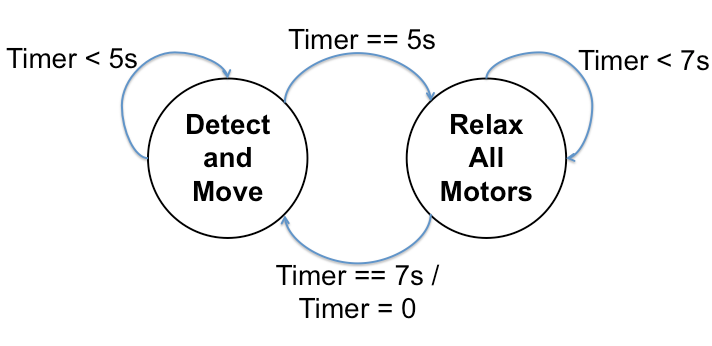
\includegraphics[width=0.7\columnwidth]{tex/img/Stepwise_state_machine/Slide1_fixed}
      \caption{Time based state machine which automates the our hand-tuned stepwise controller. Timers are used to allow for dynamic settling before the next action is taken.}
      \label{fig:stepwise_fsm}
\end{figure}

\section{Learned Neural Net Controller using Guided Policy Search}
\label{learning_nn_gps}

\todo{incorporate better}
\subsection{Mirror Descent Guided Policy Search}
\label{sec:mdgps}

Policy search algorithms aim to find a good policy by directly searching through
the space of policy parameters. Formally, we wish to find a setting of the
policy parameters $\params$ to optimize the policy
$\policy_{\params}(\at|\obs_t)$ with respect to the expected cost. In the
finite-horizon episodic setting, the expected cost under the policy is given by
$\return(\params)=\sum_{t=1}^{T}\mathbb{E}_{\policy_{\params}}[\cost(\st,\at)]$,
where $\cost(\st,\at)$ is the cost function. Here $\st$ denotes the state of our
system at time $t$, $\obs_t$ denotes the observation of the state at time $t$,
and $\at$ denotes the action at time $t$.

Guided policy search algorithms use supervised learning to train the policy,
with supervision coming from several local policies $\trajdist_i(\at|\st)$ that
are optimized to succeed only from a specific initial state of the task using
full state information. This is much simpler than the goal of the global
policy, which is to succeed under partial observability from any initial
condition sampled from the initial state distribution. These simplifications
allow the use of simple and efficient methods for training the local policies,
such as trajectory optimization methods when there is a known model, or
trajectory-centric reinforcement learning methods~\cite{la-lnnpg-14}. The
specific algorithm used in this work is MDGPS, which interprets GPS as
approximate mirror descent on $\return(\params)$~\cite{ml-gpsam-16}. The local
policies are optimized to minimize $\return(\params)$ subject to a bound on the
KL-divergence between the local policy $\trajdist_i$ and the linearization of
the global policy $\bar\policy_{\params{i}}$, following previous
work~\cite{bagnell2003covariant,ps-rlmsp-08,pma-reps-10,slmja-trpo-15}.
Optimizing the global policy is done using the samples collected in the current
iteration, which are used in a supervised fashion to approximately minimize the
divergence between the global policy and the local policies.

\setlength{\textfloatsep}{12pt}
\begin{algorithm}[tb]
    \caption{Mirror descent guided policy search (MDGPS)}
    \label{alg:mdgps}
    \begin{algorithmic}[1]
        \FOR{iteration $k = 1$ to $K$}
            \STATE Run either each $\trajdist_i$ or $\policy_{\params}$ to
            generate samples $\{\traj\}$
            \STATE Set
            $\trajdist_i\leftarrow\argmin_{\hat\trajdist_i}\mathbb{E}_{\hat\trajdist_i}[\cost(\traj)]~s.t.~D_{KL}(\hat\trajdist_i\|\bar\policy_{\params{i}})\leq\epsilon$
            \STATE Train $\policy_{\params}$ using supervised learning on
            $\{\traj\}$
        \ENDFOR
    \end{algorithmic}
\end{algorithm}

The generic MDGPS algorithm is summarized in Algorithm~\ref{alg:mdgps}. On line
2, samples are collected by running either the global policy or the local
policies. This choice between ``on-policy'' and ``off-policy'' sampling is
detailed in previous work~\cite{ml-gpsam-16}. On line 3, the algorithm improves
the local policies using an LQR-based update using fitted local linear models:
the samples are first used to fit time-varying linear dynamics for each local
policy, and these fitted dynamics are then used with a KL-constrained LQR
optimization to update the linear-Gaussian local policies. This corresponds to a
simple model-based trajectory-centric reinforcement learning method, and further
details can be found in prior work~\cite{la-lnnpg-14}. On line 4, the global
policy $\policy_\params(\at|\st)$ is updated using supervised learning, with the
training data corresponding to the states along the samples, with actions given
by the new updated local policies. This causes the global policy to ``catch up''
to the newly improved local policies, improving its behavior for the next
iteration.


\section{Optimizing Periodic Gaits with MDGPS}
\label{sec:chains}

The efficiency and speed of model-based policy optimization methods, such as the
LQR-based method used to optimize the local policies in MDGPS, is due in large
part to the fact that dynamic programming can allow for large changes to a
policy that would be impractical with purely sample-based model-free
methods~\cite{la-lnnpg-14}. However, in complex stochastic domains, such as the
contact-rich dynamical system of a rolling tensegrity robot, the accumulation of
uncertainty and variability under an unstable policy can make it difficult to
apply dynamic programming over the long horizons needed to establish a periodic
gait. We demonstrate this effect through our experimental results in
Section~\ref{sec:simresults}. In this section, we describe how we can obtain a
policy with stable periodic behavior by first splitting the task across multiple
policies, each optimized over a smaller time segment where it is easier to apply
dynamic programming, and establishing good behavior across the range of states
visited by these policies. Following the framework of GPS algorithms, we
subsequently learn a global policy that can generalize the behavior of the local
policies and encapsulate a successful periodic gait into a single policy.

GPS algorithms such as MDGPS use supervised learning to learn a global policy,
where the supervision comes from several local policies $\trajdist_i(\at|\st)$,
$i\in\{1,\ldots,C\}$. Each local policy is trained from a different initial
state, where $C$ is the chosen number of initial states. Each local policy is
optimized over $T^{\trajdist}$ time steps, and we wish to learn a global policy
$\policy_{\params}(\at|\obs_t)$ that can succeed by generalizing the behavior of
these local policies over an episode of length $T^{\policy}$. In manipulation
tasks, we usually set $T^{\policy}=T^{\trajdist}$, depending on the horizon that
we want the task to be accomplished by~\cite{lfda-eetdv-16}. In locomotion
tasks, we ideally want the global policy to exhibit continuous successful
behavior, i.e., $T^{\policy}=\infty$, and we can empirically determine
$T^{\trajdist}$ based on the amount of supervision the global policy needs to
learn a continuous periodic gait. In our work, we simply initialize
$T^{\trajdist}$ to a short horizon, and we continually increase $T^{\trajdist}$
until the global policy learns a successful locomotion gait.

If the required $T^{\trajdist}$ is long, as is the case for the \SB{} locomotion
task, it is difficult to optimize a local policy over this time horizon due to
the accumulation of uncertainty and errors described earlier. In our method, we
instead learn $L$ local policies $\trajdist_i^1,\ldots,\trajdist_i^L$ for each
initial state $i$, each optimized for $T^{\trajdist}/L$ time steps. For the
local policies $\trajdist_i^j$, $j\in\{2,\ldots,L\}$, we set the initial state
$\state_0^j$ to be the final state of the preceding local policy, i.e.,
$\state_{T^{\trajdist}/L}^{j-1}$. This amounts to training local policies in a
sequential fashion, where the $L$ local policies together are optimized over
$T^{\trajdist}$ time steps.

In previous work, the motivation behind choosing multiple initial states was so
that the global policy could succeed from all of these initial states, and
ideally generalize to other initial states as well~\cite{lfda-eetdv-16}. In our
work, we found that choosing multiple initial states is also beneficial in
learning a stable periodic gait compared to having just one initial state, and
Section~\ref{sec:simresults} demonstrates this difference. The reason for this
is that, to achieve the same amount of supervision using only one initial state,
the sequence of local policies $\trajdist_1^1,\ldots,\trajdist_1^L$ must be much
longer, and training a longer sequence increases the chances of divergence and
instability in the behavior of the local policies compared to training shorter
sequences from several stable initial states.

\setlength{\textfloatsep}{12pt}
\begin{algorithm}[tb]
    \caption{MDGPS with sequential local policies}
    \label{alg:mdgpsseq}
    \begin{algorithmic}[1]
        \FOR{iteration $k = 1$ to $K$}
            \FOR{$i = 1$ to $C$}
                \STATE $S_i\leftarrow\{\}$
                \FOR{the desired number of samples}
                    \STATE $x_0\leftarrow$ initial state $i$
                    \FOR{$l = 1$ to $L$}
                        \STATE Run either $\trajdist_i^l$ or $\policy_{\params}$ to
                        generate sample $\traj$
                        \STATE $S_i$, $x_0\leftarrow{S_i}\cup\{\traj\}$, end state of $\traj$
                    \ENDFOR
                \ENDFOR
                \FOR{$l = 1$ to $L$}
                    \STATE $\trajdist_i^l\leftarrow\argmin_{\hat\trajdist_i^l}\mathbb{E}_{\hat\trajdist_i^l}[\cost(\traj)]~s.t.~D_{KL}(\hat\trajdist_i^l\|\bar\policy_{\params{i}})\leq\epsilon$
                \ENDFOR
            \ENDFOR
            \STATE Train $\policy_{\params}$ using supervised learning on
            $\bigcup_iS_i$
        \ENDFOR
    \end{algorithmic}
\end{algorithm}

Our method is detailed in Algorithm~\ref{alg:mdgpsseq}. On line 7, we collect
samples from either the local policies or global policy. In our work, we start
by sampling from the local policies, and we switch to sampling from the global
policy after a fixed number of iterations, which we set empirically based on the
performance and stability of the local policies. On line 8, we store the
collected sample, and in order to run the policies sequentially, we set the
starting state of the next policy to be the end state of the sample $\traj$
collected from the current policy. Aside from this difference in sampling, the
rest of the algorithm is identical to MDGPS.


\section{Learning Locomotion for \SB{}}
\label{sec:superball}

For \SB{} locomotion, we chose six initial states that correspond to the stable 
ground faces that the robot traverses when rolling forward. These faces are natural 
and stable initial states that the robot may start from. We set $T^{\trajdist}=100$ and
$L=2$, so from each initial state $i$, two local policies $\trajdist_i^1$ and
$\trajdist_i^2$ are optimized over 50 time steps each, where each time step is
\SI{0.1}{\second}. We found that a fully optimized local policy can perform
about two transitions from one ground face to the next face over 5 seconds. We
also found it helpful in our work to not begin training $\trajdist_i^2$ until
$\trajdist_i^1$ trains for several iterations, so that $\state_{50}^1$, which is
$\state_0^2$, is more stable and has lower variance.  We show in
Section~\ref{sec:simresults} that training two local policies in this fashion is
much more sample efficient than training one local policy for 10 seconds, and
produces smoother and faster rolling behavior. In total, in our work, 12 local
policies are trained in sequences of two, and this provided the global policy
the supervision required to learn to roll continuously.

\subsection{Kinematic Constraints for Safe Actions}

One of the challenges with automated policy learning is that all requirements
for the policy are generally encoded in the cost function, including task-level
objectives such as desired rolling direction and hard constraints such as
safety. Due to the structure of tensegrity systems, unsafe actuation of the
motors can place the robot into configurations with unacceptable risk of cable
or motor failure. The configurations associated with such high-tension
conditions are difficult to encode analytically and even more difficult to
balance against primary task objectives in the cost function. We therefore adopt
a simple safety constraint approach to enable safe learning and policy execution
on the \SB{} hardware. This approach is challenging to use with hand-engineered
policies, which often exploit unsafe but effective actions to quickly yield a
locomotion gait. However, the approach is much easier to adopt with learned
policies, as it naturally embeds itself into the training procedure.

Specifically, we estimate the cable tensions for a particular set of actuator
positions using a simple forward kinematics model of \SB{}.  We repeat this
process for many different randomly generated motor settings and store all sets
of motor positions for which all cable tensions of the robot are below the
acceptable threshold. Then, when the policy outputs an action, we use the Fast
Library for Approximate Nearest Neighbors (FLANN)~\cite{flannsoftware} to compute
and command the nearest ($\cost_1$ norm) safe action. Computing the cable tensions
for a given set of motor positions takes a few milliseconds using forward
kinematics. As this is easily parallelized, we constructed a database containing
about 100 million motor positions deemed safe in a few hours. At runtime,
finding the nearest neighbor action takes roughly \SI{200}{\micro\second} and is
easily embedded into both training and testing without disrupting the command
frequency of \SI{10}{\hertz}.

By separating this safety constraint from the cost function, we avoid the need
to tune the parameters of the cost function to weigh the opposing objectives of
speed and hardware safety. Furthermore, we encode safety as a hard constraint
using this method, and we directly prevent unsafe actions rather than just
penalizing them. Utilizing these kinematic constraints is extremely helpful in
transferring policies learned in simulation directly onto the real robot. In
simulation, the physical limits are less restrictive, and going beyond the safe
limits does not have any adverse effects, so it is possible to train a policy
that exploits these inaccuracies in order to succeed. We can make sure this does
not happen by enforcing stronger constraints of what actions the policy can
output, and it is more likely that the policy trained with these constraints in
simulation will not fail on the real robot, or even worse, cause damage and
hardware problems.

\subsection{Generalization Across Domains}

Because we train local policies with full state information $\st$ but learn a
global policy that only receives an observation of the state $\obs_t$ as input,
we are able to train a global policy that operates under partial observability
at test time while maintaining the simplicity of training the local policies on
the full state. This separation between the local policies and global policy
reflects prior work on tasks involving partial observability, where the
intuition is that the local policies are trained in a controlled environment but
the global policy must be able to adapt to a more general
setting~\cite{lfda-eetdv-16}.

In our case, the full state $\st$ can only be obtained through either simulation
or the use of an external state estimator system on the physical \SB{}
robot~\cite{caluwaerts2016esitmation}. In contrast, we choose an observation
$\obs_t$ that can be calculated directly from the sensors on the robot itself.
This greatly simplifies the transfer from simulation to the real robot, as the
learned policy is less prone to overfit to the simulation and takes actions
directly based on the sensor measurements from the physical robot. Furthermore,
because the goal of \SB{} and many other robots is deployment to
unfamiliar, remote environments, the choice of an observation that relies only
on the robot's onboard sensors is very important, as it is unrealistic to expect
the level of information and reliability that an external state estimator can
provide. For a description of the state and observation, as well as the details
and dimensionalities of the sensors, see Section~\ref{sec:setup}.

Because the real-world sensors and actuators are noisy and imperfect, we attempt
to model this in simulation by introducing noise on the input to the policy
during training. We model measurement errors and sensor inaccuracies by adding
Gaussian noise with mean 0 and variance equal to 10\% of the range of the
observation. To model sensor failure, latency, and network issues such as
connection errors, we randomly drop observations 10\% of the time. When the
current observation is dropped, the previous observation is used as the input to
the policy. We found that adding noise improves the generalization capabilities
of the learned policy across conditions such as terrain, gravity, and motor
failure, and we test against these conditions in Section~\ref{sec:simresults}.

\section{Experimental Results}
\label{sec:results}

In our experiments, we aim to answer several questions. First, can we learn
policies in simulation that allow the simulated \SB{} to roll efficiently
under
various settings of terrain, gravity, sensor noise, and robot parameters?
Second, do our learned feedback policies generalize better to changes in
environmental and robot parameters compared to open-loop learned policies? 
Finally, can we transfer the learned policy from
simulation to the real robot, and have the real robot roll?

In Section~\ref{sec:simresults}, we establish the benefits of our method for
training sequential local policies, as well as initializing from multiple
initial states. We then test in simulation the efficiency of the learned
policies and make comparisons to establish the importance of learning and
feedback. In Section~\ref{sec:realresults}, we evaluate a learned policy on the
real robot.

\subsection{Experimental Setup}
\label{sec:setup}

We encode the state of the system $\st$ as the position and velocity of each of
the 12 bar endpoints of \SB{}, and the position and velocity of each of the 12
motors, measured in radians, for a total dimensionality of 96. We experimented
with two different representations for the observation $\obs_t$. The ``full''
36-dimensional observation includes motor positions, and also uses elevation and
rotation angles calculated from the accelerometer and magnetometer sensors on
the robot. The ``limited'' observation is 12-dimensional and only uses the
acceleration measurement along the bar axis from each of the accelerometers. We
found that interfering magnetic fields near the testing grounds at NASA
Ames cause the magnetometers to be unreliable and difficult to calibrate, and
because of this, the policy using the limited observation is much easier to
transfer on to the real robot. The action $\at$ is the instantaneous desired position 
of each motor. 

For our task, each local policy requires about 200 samples before they are
reliably successful. Simultaneously during training of the local policies, we
learn a global policy, which in our work is a deep neural network with three
hidden layers of 64 rectified linear units (ReLU) each, using the same samples.
Our cost function $l(\st,\at)$ is simply the negative average velocity
of the bar endpoints of the robot, so that the local policies are trained to
roll as quickly as possible.

\subsection{Results in Simulation}
\label{sec:simresults}

\begin{table*}[t]
    \centering
    \resizebox{\textwidth}{!}{%
        \begin{tabular}{|llrrrrr|}
            \hline
            \multicolumn{5}{|c|}{}                                                                                                                                                                                                                                                                                  & \multicolumn{2}{c|}{} \\
            \multicolumn{2}{|c}{}                                                        & \multicolumn{3}{c|}{\multirow{-2}{*}{\textbf{Our Method}}}                                                                                                                                                               & \multicolumn{2}{c|}{\multirow{-2}{*}{\textbf{Open-Loop}}} \\
            \multicolumn{2}{|c}{}                                                        & \multicolumn{1}{r|}{Full Observation,}                                 & \multicolumn{1}{r|}{Limited Observation,}                              & \multicolumn{1}{r|}{Limited Observation,}                              & \multicolumn{1}{r|}{Mean Actions from}                           & Hand-Engineered \\
            \multicolumn{2}{|c}{}                                                        & \multicolumn{1}{r|}{Six Initial States}                                & \multicolumn{1}{r|}{Six Initial States}                                & \multicolumn{1}{r|}{One Initial State}                                 & \multicolumn{1}{r|}{Best Learned Policy}                         & Punctuated Rolling \\
            \cline{3-7}
            \multicolumn{2}{|l}{}                                                        & \multicolumn{1}{r|}{}                                                  & \multicolumn{1}{r|}{}                                                  & \multicolumn{1}{r|}{}                                                  & \multicolumn{1}{r|}{}                                            & \\
            \multicolumn{2}{|l}{\multirow{-2}{*}{\textbf{Normal Conditions}}}            & \multicolumn{1}{r|}{\multirow{-2}{*}{$\mathbf{25.307\pm0.309}$}}       & \multicolumn{1}{r|}{\multirow{-2}{*}{$24.141\pm0.352$}}                & \multicolumn{1}{r|}{\multirow{-2}{*}{$20.008\pm0.871$}}                & \multicolumn{1}{r|}{\multirow{-2}{*}{$\mathit{25.076\pm0.078}$}} & \multirow{-2}{*}{$10.266\pm0.071$} \\
            \rowcolor[HTML]{D3D3D3}
            \cellcolor[HTML]{D3D3D3}                                   & Rocky           & \multicolumn{1}{r|}{\cellcolor[HTML]{D3D3D3}$\mathit{6.025\pm2.835}$}  & \multicolumn{1}{r|}{\cellcolor[HTML]{D3D3D3}$\mathbf{9.568\pm5.197}$}  & \multicolumn{1}{r|}{\cellcolor[HTML]{D3D3D3}$3.124\pm1.083$}           & \multicolumn{1}{r|}{\cellcolor[HTML]{D3D3D3}$3.069\pm2.201$}     & $1.734\pm0.411$ \\
            \rowcolor[HTML]{D3D3D3}
            \cellcolor[HTML]{D3D3D3}                                   & Uphill          & \multicolumn{1}{r|}{\cellcolor[HTML]{D3D3D3}$\mathbf{18.547\pm0.231}$} & \multicolumn{1}{r|}{\cellcolor[HTML]{D3D3D3}$\mathit{16.107\pm0.809}$} & \multicolumn{1}{r|}{\cellcolor[HTML]{D3D3D3}$13.573\pm0.174$}          & \multicolumn{1}{r|}{\cellcolor[HTML]{D3D3D3}$7.721\pm0.236$}     & $8.136\pm0.026$ \\
            \rowcolor[HTML]{D3D3D3}
            \multirow{-3}{*}{\cellcolor[HTML]{D3D3D3}\textbf{Terrain}} & Downhill        & \multicolumn{1}{r|}{\cellcolor[HTML]{D3D3D3}$\mathbf{32.896\pm0.275}$} & \multicolumn{1}{r|}{\cellcolor[HTML]{D3D3D3}$\mathit{29.970\pm0.858}$} & \multicolumn{1}{r|}{\cellcolor[HTML]{D3D3D3}$21.963\pm2.403$}          & \multicolumn{1}{r|}{\cellcolor[HTML]{D3D3D3}$27.661\pm0.136$}    & $11.264\pm0.091$ \\
                                                                       & 10\%            & \multicolumn{1}{r|}{$\mathbf{19.505\pm0.746}$}                         & \multicolumn{1}{r|}{$16.966\pm0.362$}                                  & \multicolumn{1}{r|}{$13.927\pm0.516$}                                  & \multicolumn{1}{r|}{$\mathit{18.024\pm2.356}$}                   & $11.044\pm0.054$ \\
                                                                       & 50\%            & \multicolumn{1}{r|}{$\mathbf{23.331\pm0.871}$}                         & \multicolumn{1}{r|}{$\mathit{21.220\pm0.202}$}                         & \multicolumn{1}{r|}{$17.766\pm0.490$}                                  & \multicolumn{1}{r|}{$19.673\pm3.244$}                            & $10.310\pm0.010$ \\
            \multirow{-3}{*}{\textbf{Gravity}}                         & 200\%           & \multicolumn{1}{r|}{$\mathbf{27.600\pm2.307}$}                         & \multicolumn{1}{r|}{$\mathit{26.715\pm0.566}$}                         & \multicolumn{1}{r|}{$21.680\pm1.330$}                                  & \multicolumn{1}{r|}{$24.865\pm0.190$}                            & $9.845\pm0.009$ \\
            \rowcolor[HTML]{D3D3D3}
            \cellcolor[HTML]{D3D3D3}                                   & Heavy           & \multicolumn{1}{r|}{\cellcolor[HTML]{D3D3D3}$12.521\pm1.710$}          & \multicolumn{1}{r|}{\cellcolor[HTML]{D3D3D3}$\mathbf{14.561\pm0.079}$} & \multicolumn{1}{r|}{\cellcolor[HTML]{D3D3D3}$\mathit{12.972\pm0.110}$} & \multicolumn{1}{r|}{\cellcolor[HTML]{D3D3D3}$1.081\pm0.019$}     & $10.550\pm0.003$ \\
            \rowcolor[HTML]{D3D3D3}
            \multirow{-2}{*}{\cellcolor[HTML]{D3D3D3}\textbf{Robot}}   & End Cap Failure & \multicolumn{1}{r|}{\cellcolor[HTML]{D3D3D3}$\mathit{21.890}$}         & \multicolumn{1}{r|}{\cellcolor[HTML]{D3D3D3}$\mathbf{22.100}$}         & \multicolumn{1}{r|}{\cellcolor[HTML]{D3D3D3}$ $}                       & \multicolumn{1}{r|}{\cellcolor[HTML]{D3D3D3}$10.291$}            & $10.247$ \\
                                                                       & 0\%             & \multicolumn{1}{r|}{$\mathbf{26.494}$}                                 & \multicolumn{1}{r|}{$\mathit{25.828}$}                                 & \multicolumn{1}{r|}{$ $}                                               & \multicolumn{1}{r|}{}                                            & \\
            \multirow{-2}{*}{\textbf{Added Noise}}                     & 20\%            & \multicolumn{1}{r|}{$\mathit{7.725}$}                                  & \multicolumn{1}{r|}{$\mathbf{19.212}$}                                 & \multicolumn{1}{r|}{$ $}                                               & \multicolumn{1}{r|}{\multirow{-2}{*}{N/A}}                       & \multirow{-2}{*}{N/A} \\
            \hline
        \end{tabular}%
    }
    \caption{
        \label{table:distance}
        Average distances in meters traveled using the policies learned through
        our method with varying observation representations and local policy
        training schemes, the open-loop mean actions from the learned policy
        that performs best under training conditions, and the hand-engineered
        open-loop policy. Results are averaged across five trials of one minute
        each for a variety of terrain, gravity, noise, and robot settings.
        ``Normal Conditions'' are the training conditions, which are flat
        terrain, 100\% gravity, 10\% added noise to the input, and normal robot
        parameters. When varying one setting, all other settings remain the same
        as during training time. We do not test the open-loop controllers with
        varying input noise, because these controllers do not have any input.
        Bolded numbers indicate the farthest distance traveled for any given
        condition, and italicized numbers are the second farthest. Note that the
        first two learned policies generally outperform all other controllers,
        demonstrating the benefits of our method and using multiple initial
        states in learning efficient and generalizable locomotion.
    }
\end{table*}

The \SB{} simulation that we use is built off of the NTRT open-source project.
Aside from speed and efficiency benefits, the simulation also allows us to
systematically and easily vary the parameters of the robot and environment.

To show that our method of training sequential local policies is effective, we
compared the results of training two sequential local policies for 5 seconds
each against training one local policy for the full 10 seconds, both using the
trajectory-centric reinforcement learning method detailed in~\cite{la-lnnpg-14}.
The average distance traveled over five trials for the two \SI{5}{\second} local polices and the 
single \SI{10}{\second} policy were \SI{3.15}{\meter} and \SI{1.23}{\meter}, respectively.
%We record the average distance traveled over five trials in
%Table~\ref{table:chains}. 
These results demonstrate that, by training sequences
of local policies over shorter horizons, we can achieve more efficient
locomotion with fewer samples by decreasing the accumulation of error over time.

To demonstrate the benefit of multiple initial states, we also use our method to
learn a global policy using one long sequence of six local policies, trained
over \SI{5}{\second} each, starting from only one initial state. 
These six polices encapsulated a full rotation of the robot.
We were unable to
successfully train %the 5th local policy to continue the gait, due to both the
a full roll due to the
build-up in variance in the starting states of the local polices and the
divergence in the behavior of the local policies from the desired periodic gait.
%The global policy learns a gait from the 4 local policies that were trained
%successfully, but the resulting behavior is less efficient and also
%significantly less stable, as the policy will sometimes diverge from a stable
%periodic gait, at which point it fails to continue making forward progress.

Our results for testing the learned policies against a range of environmental
and robot parameters are presented in Table~\ref{table:distance}. We report the
average distance traveled over five trials of \SI{60}{\second} for three policies
learned with MDGPS, an open-loop policy that outputs the mean actions from the
learned policy that performs best under training conditions, and an open-loop
hand-engineered controller. The policies learned with MDGPS use either the
36-dimensional observation, or the 12-dimensional observation. 
As discussed earlier, we also learn a policy using the accelerometer
observation and a long sequence of local policies from one initial state
%, to
%compare this against policies learned using several shorter sequences starting
%from multiple initial states. 
The open-loop hand-engineered controller is
designed to follow the basic locomotion strategy described in
Section~\ref{sec:tensegrity}.

%We systematically vary a suite of settings in simulation: the ground terrain,
%which can be flat, uneven, or sloped up or downhill; the strength of the
%gravitational field, which can be 10\%, 50\%, 100\%, or 200\% of Earth's
%gravity; the noise level on the inputs to the policy, which can be 0\%, 10\%,
%and 20\%; and various parameters of the robot. For robot parameters, we increase
%the mass of the rods and decrease the maximum motor velocities to create a
%heavier robot, and we simulate the failure of a specific end cap by dropping all
%sensors readings and motor commands.

The learned policy with full observation performs best under training
conditions, and also demonstrates the best generalization across terrain and
gravity settings as well as the noiseless condition. The learned policy with
limited observation, though slightly less efficient than the policy with full
observation, adapts better to the heavier robot as well as to motor failure, and
also performs significantly better under heavy noise. These conditions are
important for successful transfer to the real world setting, since the
parameters of the physical \SB{} robot naturally differ from the simulation, and
the imperfections in the hardware result in sensor and motor unreliability. We
show the success of this learned policy in transferring onto the real robot in
Section~\ref{sec:realresults}. The learned policy from the single long sequence
of local policies does not perform as well as the other learned policies,
because it is prone to diverge and become instable, at which point it fails.

The open-loop mean actions from the learned policy demonstrate comparable
results under the training conditions, as expected, but its performance falls
off drastically for most of the other conditions. 
%Because a controller for \SB{}
%would ideally work under different terrains and in the presence of hardware
%issues, this shows that it is imperative that we use a closed-loop
%representation to ensure successful and reliable locomotion. 
The hand-engineered
open-loop controller rolls consistently across most conditions, but is
significantly less efficient than the three other policies. This emphasizes the
benefits of learning and the difficulty in hand-engineering good controllers, as
this controller was carefully designed but still sacrifices speed and other
important benefits, such as robot safety, for reliability. Most notably, this
hand-engineered controller has caused motor and cable failure on the physical
\SB{} robot in the past, which is why we did not compare against it for the real
robot results.

In summary, these results show that all learned policies substantially
outperform the hand-engineered rolling controller, and the closed-loop neural
network policies outperform the open-loop baselines in almost all conditions,
indicating the benefits of both learning and feedback in \SB{} locomotion. Our
method is able to learn successful and efficient policies even with the limited
sensory observations provided by only \SB{}'s accelerometers, and the learned
policies demonstrate generalization to unseen conditions representative of what
a planetary exploration rover might encounter, such as changing terrains,
unstable levels of noise, and hardware failure. The addition of input noise
during training encourages this generalization, and results in learned policies
with similar levels of reliability as the hand-engineered controller, though
significantly faster and less likely to cause hardware failure on the real
robot.

\subsection{Results in the Real World}
\label{sec:realresults}

We compared the learned policy with limited observation, trained in simulation,
against an open-loop policy that outputs the mean actions from this learned
policy under training conditions. Both policies were run on the physical \SB{}
robot on flat terrain. Videos of the training process and experiments can be
found on the project
website.\footnote{\url{http://rll.berkeley.edu/drl\_tensegrity}}

Over three trials of 100 seconds each, using the learned policy, \SB{} rolled
approximately \SI{12}{\meter}, \SI{9}{\meter}, and \SI{8}{\meter}.
\SI{12}{\meter} is about the maximum distance allowed during the trials, as the robot rolled 
out side our limited network range and could not roll any further.
%, for an
%average distance of \SI{9.7}{\meter}, with a standard deviation of
%Various hardware issues impeded the robot from traveling
%further. 
%The connection between the robot and the computer running the policy
%was strained as the robot traveled farther away, and as a result sensor readings
%and motor commands were dropped. 
Also, a cable malfunction cut the last
trial short by about 20 seconds, which was on track to reach the \SI{12}{\meter} limit. 
Despite these issues and the differences
between the simulated and physical robot, the policy was able to successfully
produce a gait on \SB{} that is more reliable, and less risky for
the hardware, than any previous locomotion controller.
The learned policy is able to adapt to the
physical \SB{} robot by using feedback from the accelerometers, as seen in 
figure~\ref{fig:commands}.

\begin{figure}[thpb]
    \centering
    \setlength{\unitlength}{0.5\columnwidth}
    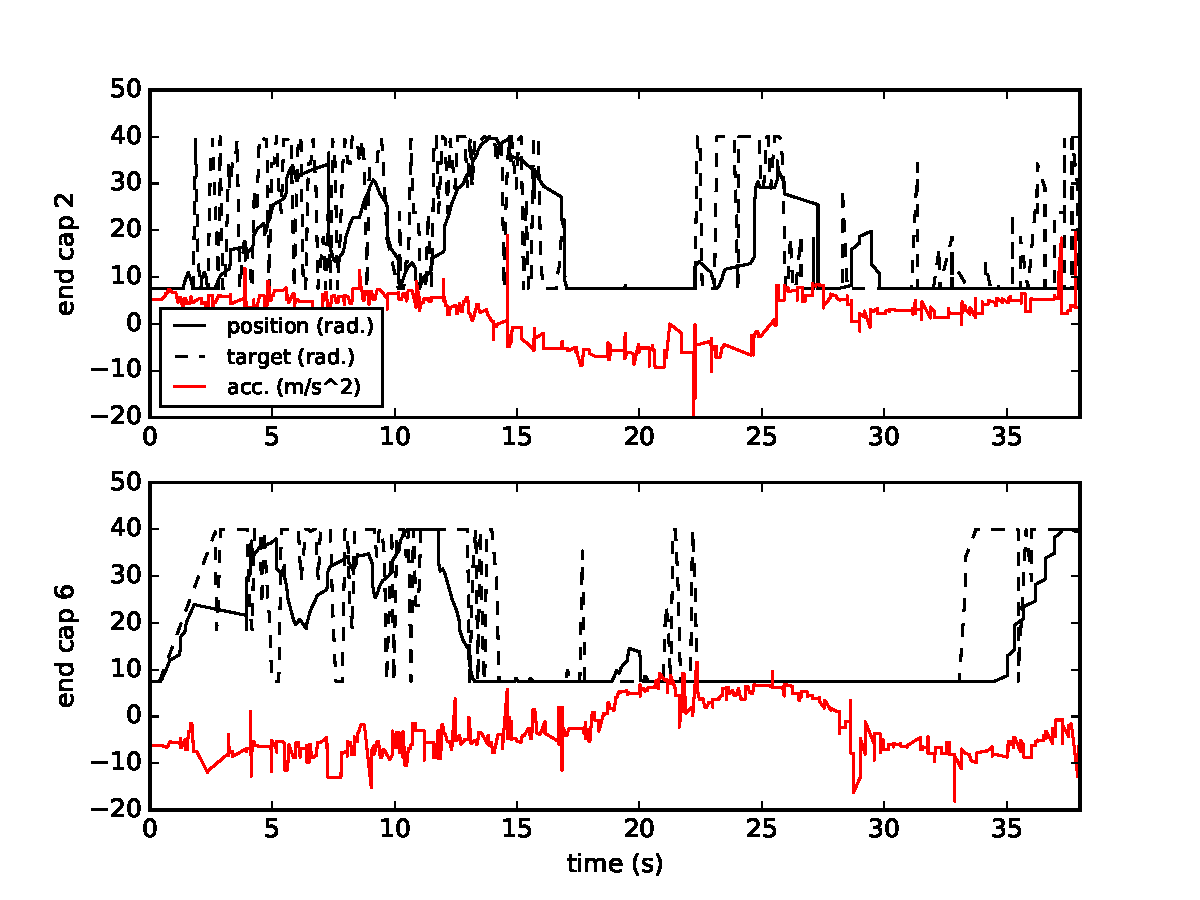
\includegraphics[width=\linewidth]{tex/img/plot_motor}
    \caption{
        \label{fig:commands}
        This plot shows actual motor positions, target motor positions, and 
        single axis accelerometer data over the first 40 seconds of a trial
        for two rod ends which are not connected via cables and not attached
        to the same rod. The commanded positions change based on
        the accelerometer feedback, showing the controller working as the robot
        changes orientation by rolling. The actual motor position  
        lags behind the target motor position due to motor dynamics and network UDP packet loss.
    }
\end{figure}

The open-loop policy was not able to produce any reasonable behavior on the real
robot, and we ran it only once due to concerns about hardware safety. 
%The lack
%of performance and safety exhibited by this policy can be explained by viewing
%the difference in motor commands sent by the learned policy in simulation and on
%the real robot, shown in Figure~\ref{fig:commands}. 
Due to various modeling
imprecisions, the simulated \SB{} has a greater maximum motor velocity, and the
policy uses this discrepancy to achieve faster locomotion. The open-loop policy
attempts to mimic this on the real robot, which does not work because the robot
cannot reach the same motor positions over a fixed number of time steps as in
simulation. 
%In addition, despite following all of the action constraints, the
%open-loop policy is dangerous for the cables because they are frayed by the
%constant expansion and contraction. 
%and we can see that it
%adopts a strategy that applies motor commands for a longer period of time in
%order to move the robot into the desired configuration and produce a successful
%locomotion gait.


\section{CPG or Other Controller}
\label{cpg_controller}

\section{Dynamic Rolling}
\label{dyncamic_rolling}
\chapter{Current and Future Work}

\section{\SB{} Current State}
At this point, the first goal proposed in section \ref{goal} has been achieved.
\SB{} is composed of twelve Modular Tensegrity Robots (MTR) attached as the ends of 6 rods connected in a icosahedron geometry, and may be seen in figure \ref{fig:SB}.
Preliminary testing of the system, presented in the following sections, has shown many of the basic functions and features that will enable goals two and three.
All data collected in this section was collected through the wireless ROS network with no extra sensors or equipement apart from what was designed into the system, explained in chapter \ref{design}. 

\subsection{Dynamic Torque Sensor Testing}
\begin{figure}[thpb]
      \centering
      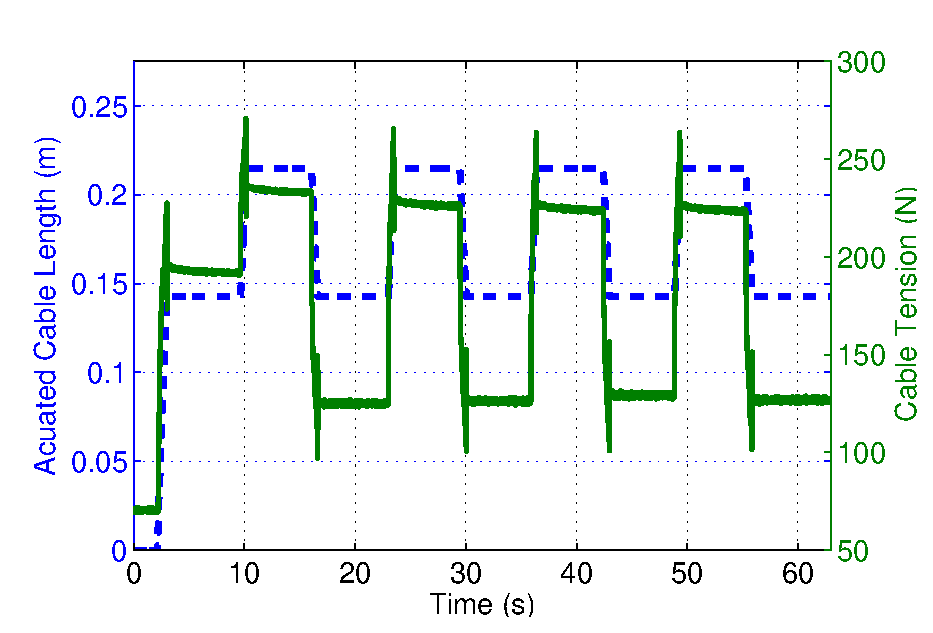
\includegraphics[width=0.8\columnwidth]{tex/img/ICRA2015_dynamic_sensor_test}
      \caption{Motor mount torque sensor data and motor position data recorded during a square wave input position trajectory for a single motor. This plot shows measured tension from the sensor and cable length from motor encoder measurements as a function of time for this dynamic movement.}
      \label{fig:sensor1data}
\end{figure}

This test was performed to demonstrate the force sensors' ability to capture data under dynamic motion.
Figure~\ref{fig:sensor1data} shows a plot of sensor data from one end cap whose motor is commanded in a square-wave position trajectory.
The position trajectory had a period of \SI{13}{\second}, and oscillated between \SI{10}{\radian} and \SI{15}{\radian} of the output shaft measured before the gearbox, by the encoder.
The trajectory of sensor torque values reasonably tracks the position square wave: the commanded position trajectory starts at 10 seconds and ends at 62 seconds, as does the sensed tension square wave.
The overshoot on the torque sensor measurements is due to the system inertia and spring dynamics.

\subsection{Global Force Redistribution Sensor Testing}

\begin{figure}[thpb]
      %\vspace{-0.5cm}
      \centering
      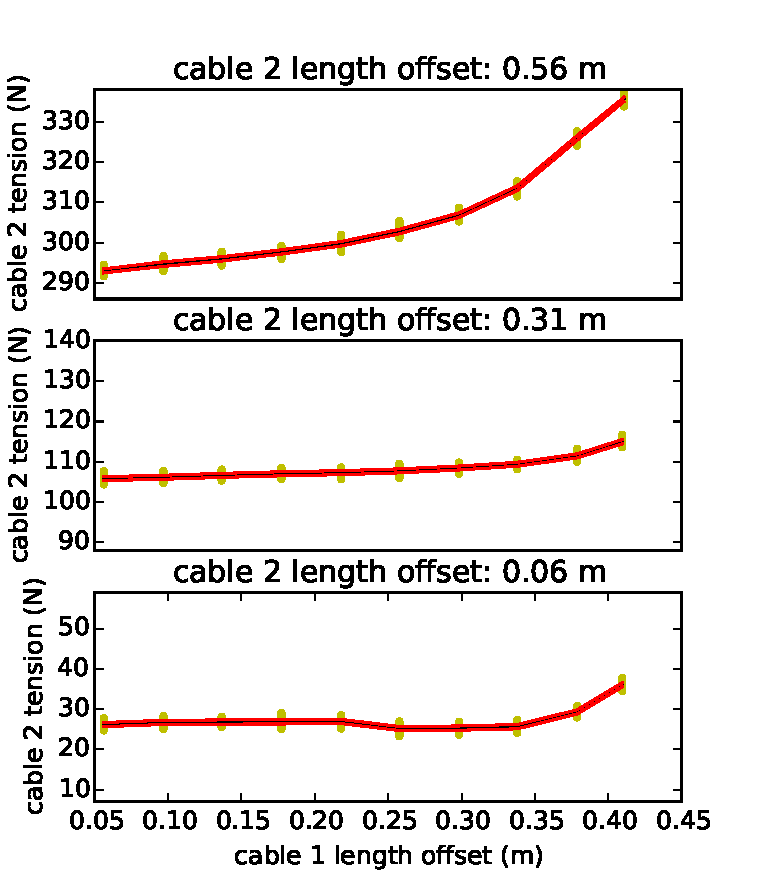
\includegraphics[width=0.55\columnwidth]{tex/img/sensor2_original}
      \caption{Global force redistribution test. Yellow marks are the means of roughly 5,000 tension sensor measurements of \emph{cable 2} opposite that which is actuated (\emph{cable 1}.) The black line shows the linear interpolation between points, with the red boundary as standard deviation. The pretension in the sensed cable is adjusted in each test, showing measurement sequences at increasing pretensions.}
      \label{fig:sensor2data_forcedistribution}
\end{figure}

A test was performed to validate the distribution of tension throughout the system, and to show that all sensors can work in conjunction simultaneously.
Figure~\ref{fig:sensor2data_forcedistribution} shows tension readings from a different motor-mount torque sensor on the opposite side of \SB{} (Cable 2) from a cable which is being retracted (Cable 1.)
Cable 2 was not actively actuated during each test.
For each plot in Figure~\ref{fig:sensor2data_forcedistribution}, the actuated cable was retracted with various step inputs marked in the figure.
Each data point in this figure (yellow) was collected by averaging data from the sensor board for a total of 5 seconds at 1 kHz, after waiting 2 seconds after the step input actuation to avoid dynamic effects.
These tests were done with different levels of pretension on the sensed cable: this pretension was adjusted by changing the length of the sensed cable.
Though the lower-pretension tests show smaller changes in readings, the higher pretensions show increasing readings which demonstrate the ability to sense forces throughout the tension network in pseudo-equilibrium states, as well as \SB{}'s passive force redistribution properties.

\subsection{Basic Locomotion}
\label{basic_locomotion}
Using a basic step input to a single motor, \SB{} can perform a simple transition from one face of the icosahedron to another.
Figure \ref{fig:superball_flop_flat} shows an test where a motor retracts a cable, induing a flop.
The idea of this type of simple transition is to deform the base equilateral triangle such that the center of mass "moves" over the triangle's edge.
The robot becomes unstable and gravity pulls the system over.
The momentum of the system then rolls the robot through the adjacent isosceles triangle to the next equilateral triangle.
In this test, the motor retraction was preset and experimentally derived earlier.

\begin{figure}[t]
    \centering
    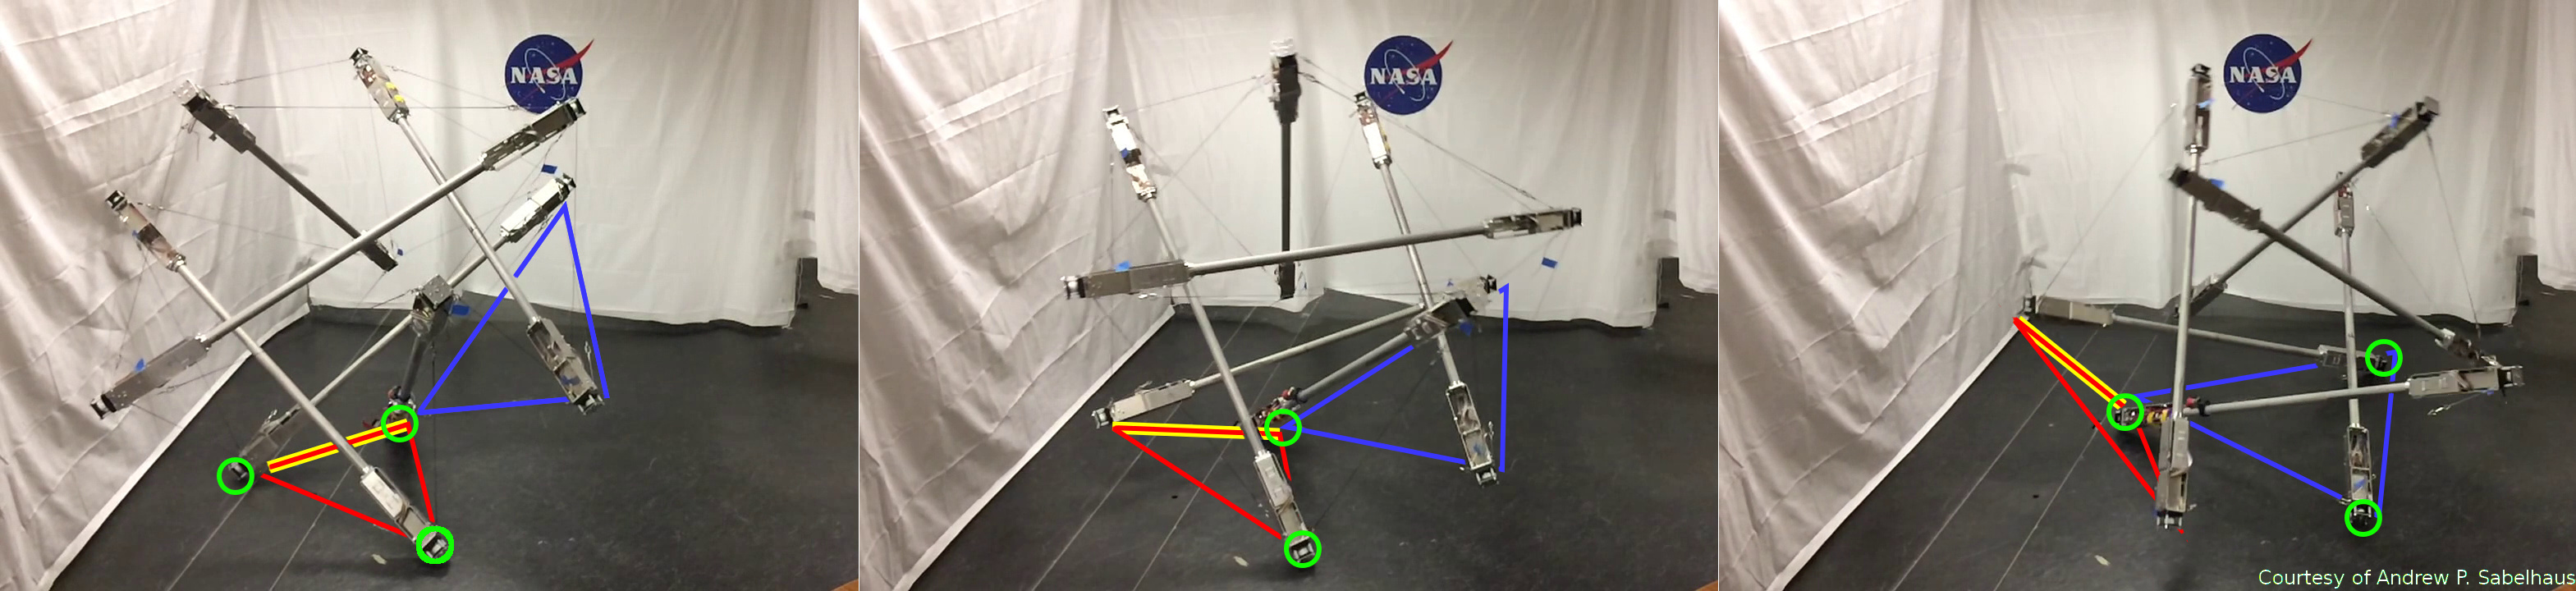
\includegraphics[width=1\linewidth]{tex/img/superball_flop_combined_betterlabels}
    \caption{\SB{} performing a single face-change movement, from one equilateral triangular face to another. The robot begins with all MTRs of the red triangle touching the ground. Then, \SB{} retracts the yellow-highlighted cable on the red triangle, inducing movement. Frame 2 shows \SB{} halfway through the movement with only two points of contact on the ground. Finally, frame 3 shows \SB{} at the end, with all 3 points of the blue triangle in ground contact.}
    \label{fig:superball_flop_flat}
\end{figure}

\section{Future Work}

%\subsection{Proposed Controls Methods}

\subsection{Open Loop Locomotion Control}
\label{open_loop}
For clarity, open loop used here is open in regards to the locomotion system's ability to change robotic motor inputs based on environmental sensing.
Work presented in~\cite{iscen2014flop} shows through simulation that a tensegrity system like \SB{} can achieve a rolling gait by deforming the triangle currently in contact with the ground.
Though \SB{} is not fully actuated (all 24 external cables are attached to motors), a derivative of this work may be able to be applied to \SB{}.
Leveraging the experimental results from section \ref{basic_locomotion}, \SB{} can achieve open loop locomotion quite easily with the addition of detecting which face of the robot is on the ground.
To achieve this ground detection, I propose to use the IMU modules on each sensor board to detect earth's gravity field and/or ground contacts when a rod contacts the ground.
Using a basic machine learning technique, like k-nearest neighbor, may enable successful classification of where the ground is in relation to the robot.

\subsection{Closed Loop Locomotion Control}
There has been preliminary results done by~\cite{burms2015online} which demonstrates a tensegrity robot sensing different enviromental terrains.
This shows promise that a tensegrity robot may sense changes in terrain without the need for extra sensors.
If a similar technique can be achieved on \SB{} in a real-time manor, then the open loop gait pattern used from \ref{open_loop} can be altered to better locomote over the sensed terrain.
This new locomotion gait may either be hand tuned parameters or learned behavior.

\begin{appendices}
\chapter{\SB{} v1 Design Evaluation}
\label{app:evalutation}

Once \SB{} v1 was built and evaluated, the system performed mostly as designed.
Since this was an initial venture into building an untethered tensegrity robot, there were several design choices that ultimately impacted the system's performance negatively.
In the following sections, I will try to summarize and evaluate how the mechanical, electrical, and communication systemnjous performed.
I will then try to make suggestions to improve upon these systems.

\section{Mechanical Evaluation}

In this section, an evaluation of the \SB{} will be taken based on the three main subsystems outlined above.

\subsection{Cable Routing}
Upon testing and using \SB{}, the limitations on the mechanical design became the largest hindrance to achieving consistent performance.
A large majority of the mechanical limitations stemmed from the bowden cable routing, management, and material choices.
The design of the MTR was focused around using a bowden system to route cables around components and features within the housing.
This allowed for the cable routing to be secondary to the placement of components within the MTR, making the overall design easier, but increasing the number of bends in the bowden cable housing.
As explained in section \ref{routing}, the internal cable material used was braided steel cable.
The steel cable allowed for easy assembly and good wear resistance, however it has a minimum bend radius to keep the cable from plastically deforming.
Our initial design took into account this limitation with a correctly sized roller guide (see figure \ref{fig:roller_guide}), though in practice the combination of the induced tension and the wrong type of groove in the roller guide leads to a slight plastic deformation of the steel cable in the form of kinks.
Extra friction is then imparted into the bowden system as theses kinks try to slide inside the bowden housing.
Friction between the cable and housing element was a known factor, however the amount of friction it induced is much larger than expected.
Figure \ref{fig:cable_friction} shows a qualitative example of hysteresis in cable length due to the effect friction has on the system.

% \begin{figure}[thpb]
%       \centering
%       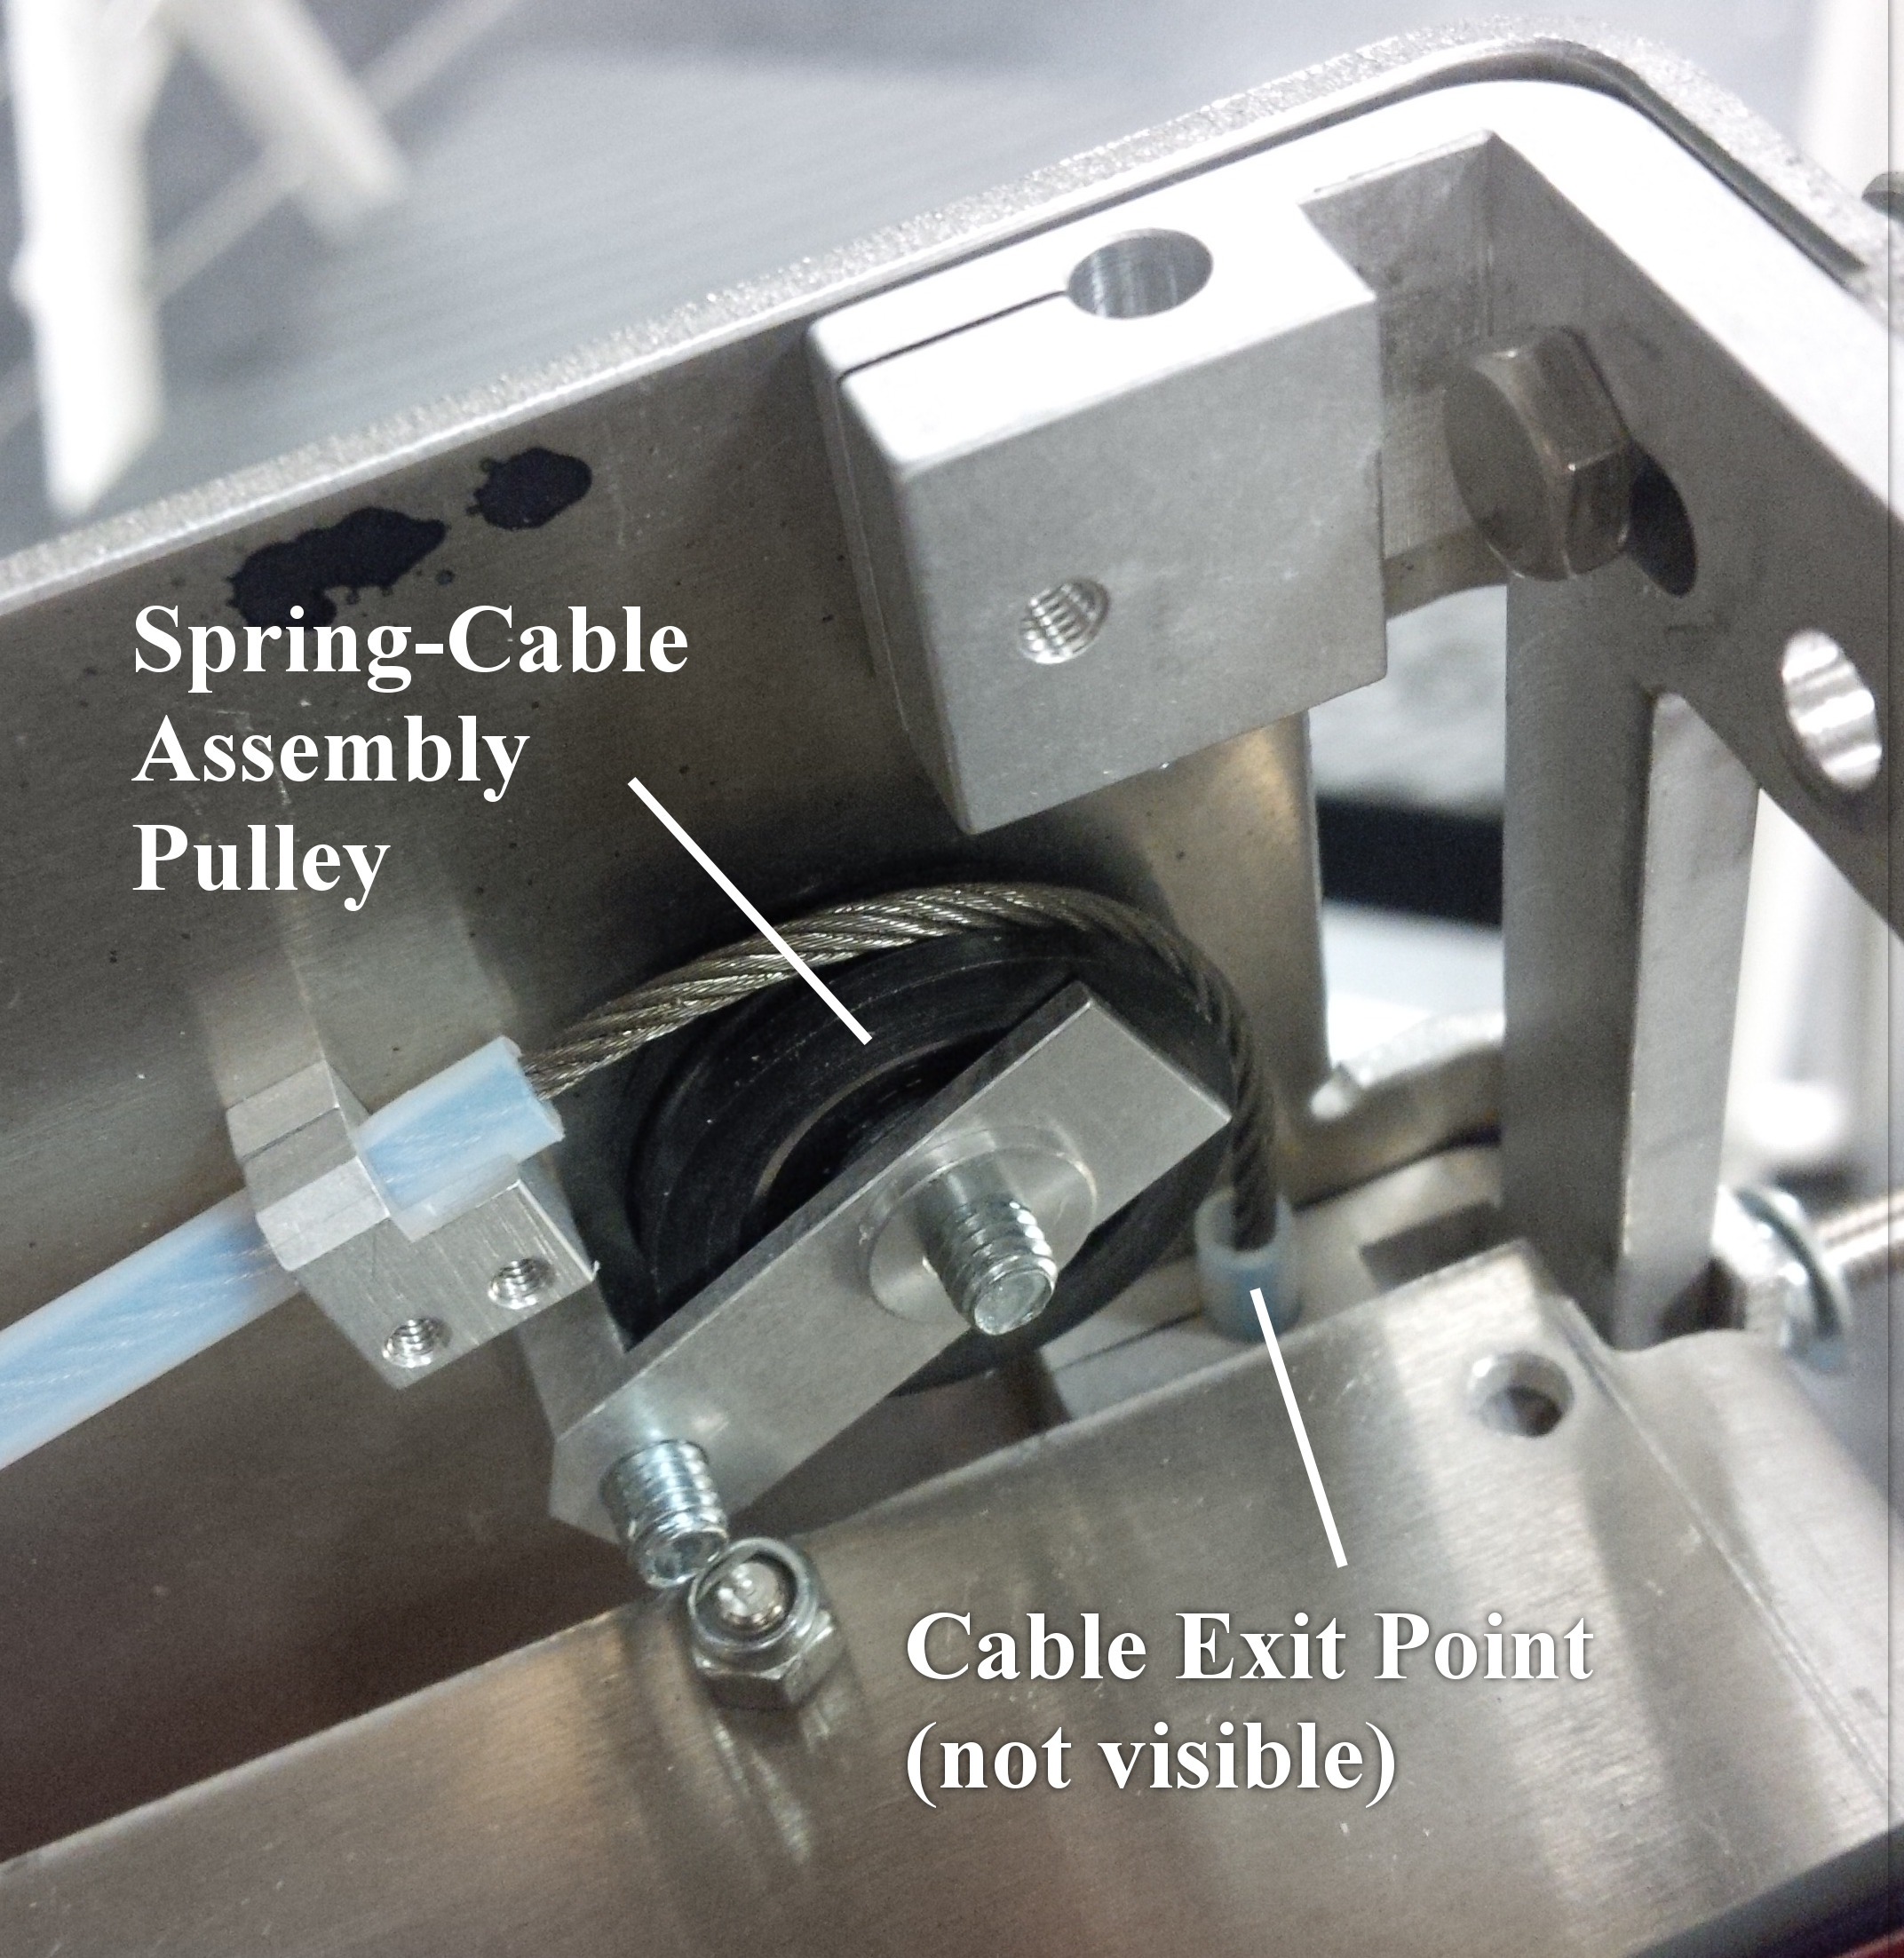
\includegraphics[width=0.6\columnwidth]{tex/img/cable_pulley_bearing_labelled_fixedfonts}
%       \caption{\textcolor{red}{Temp. figure. Explain how the pictures show hysteresis due to cable friction.}}
%       \label{fig:cable_friction}
% \end{figure}

\begin{figure}[htp] % not h only
\centering
\begin{subfigure}{.5\textwidth}
\centering
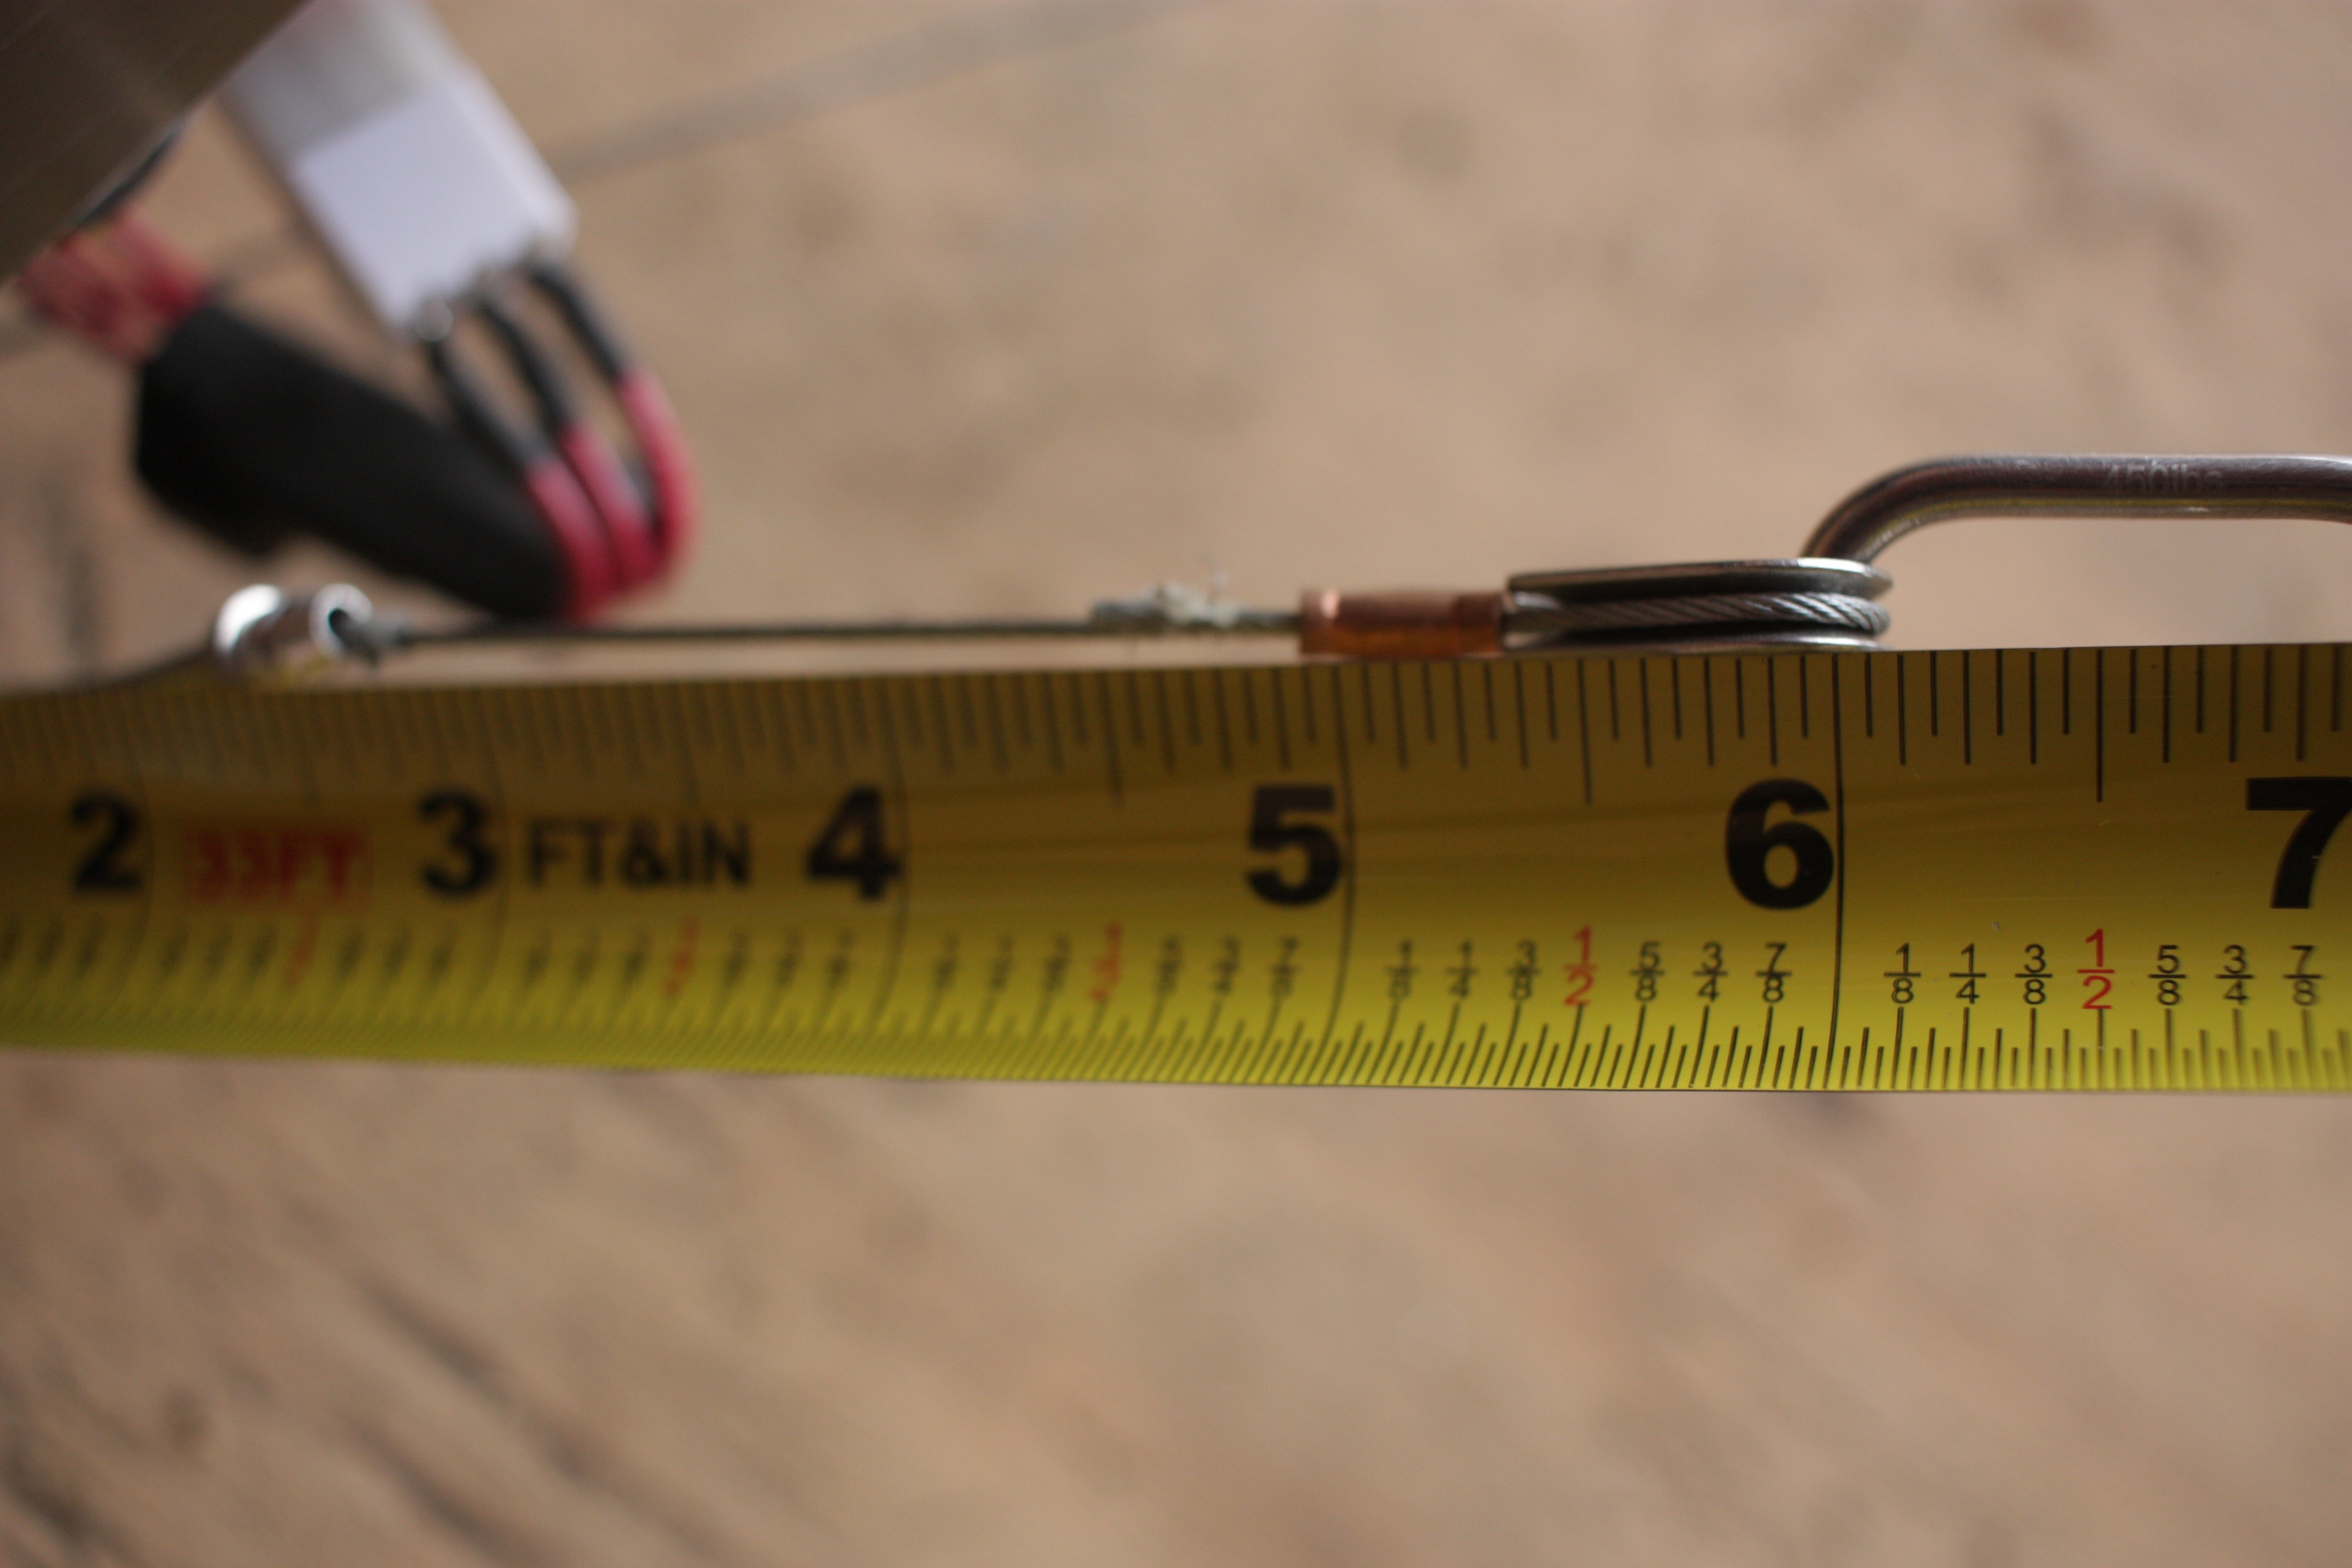
\includegraphics[width=0.9\linewidth]{tex/img/ruler_6}%
\label{fig:ruler_6}%
\end{subfigure}%
\begin{subfigure}{.5\textwidth}
\centering
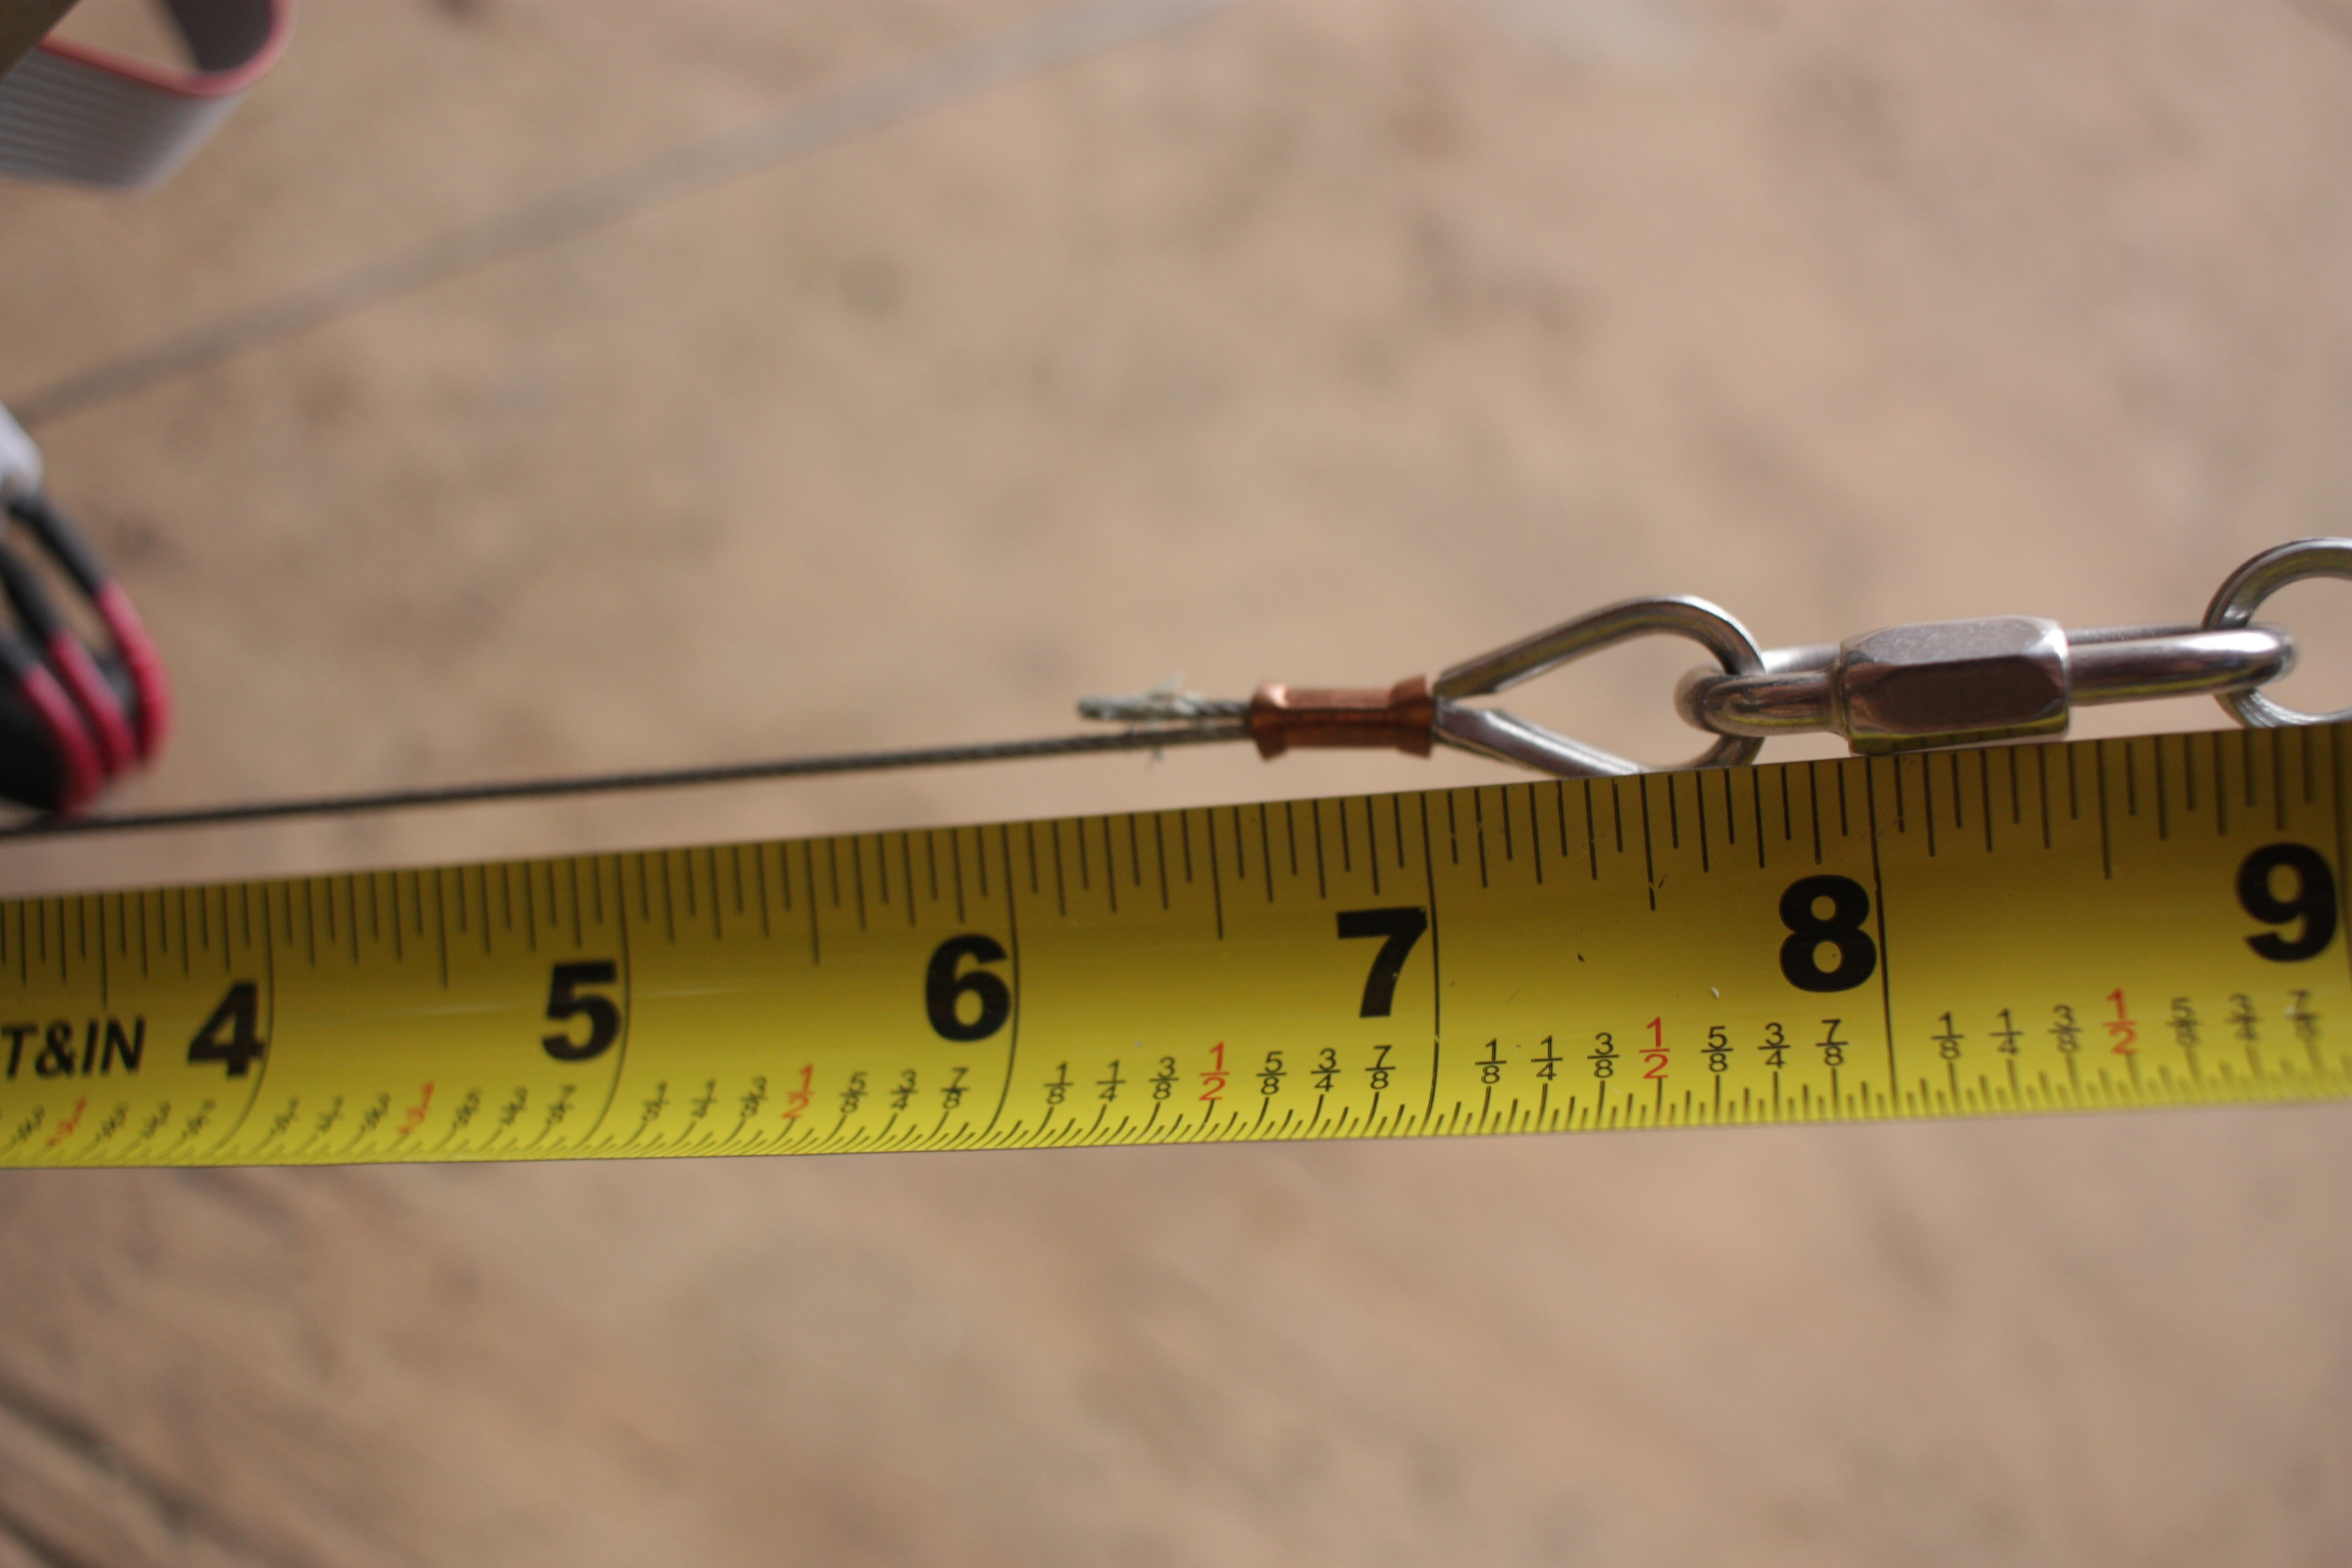
\includegraphics[width=0.9\linewidth]{tex/img/ruler_8}%
\label{fig:ruler_8}%
\end{subfigure}%

\begin{subfigure}{.5\textwidth}
\centering
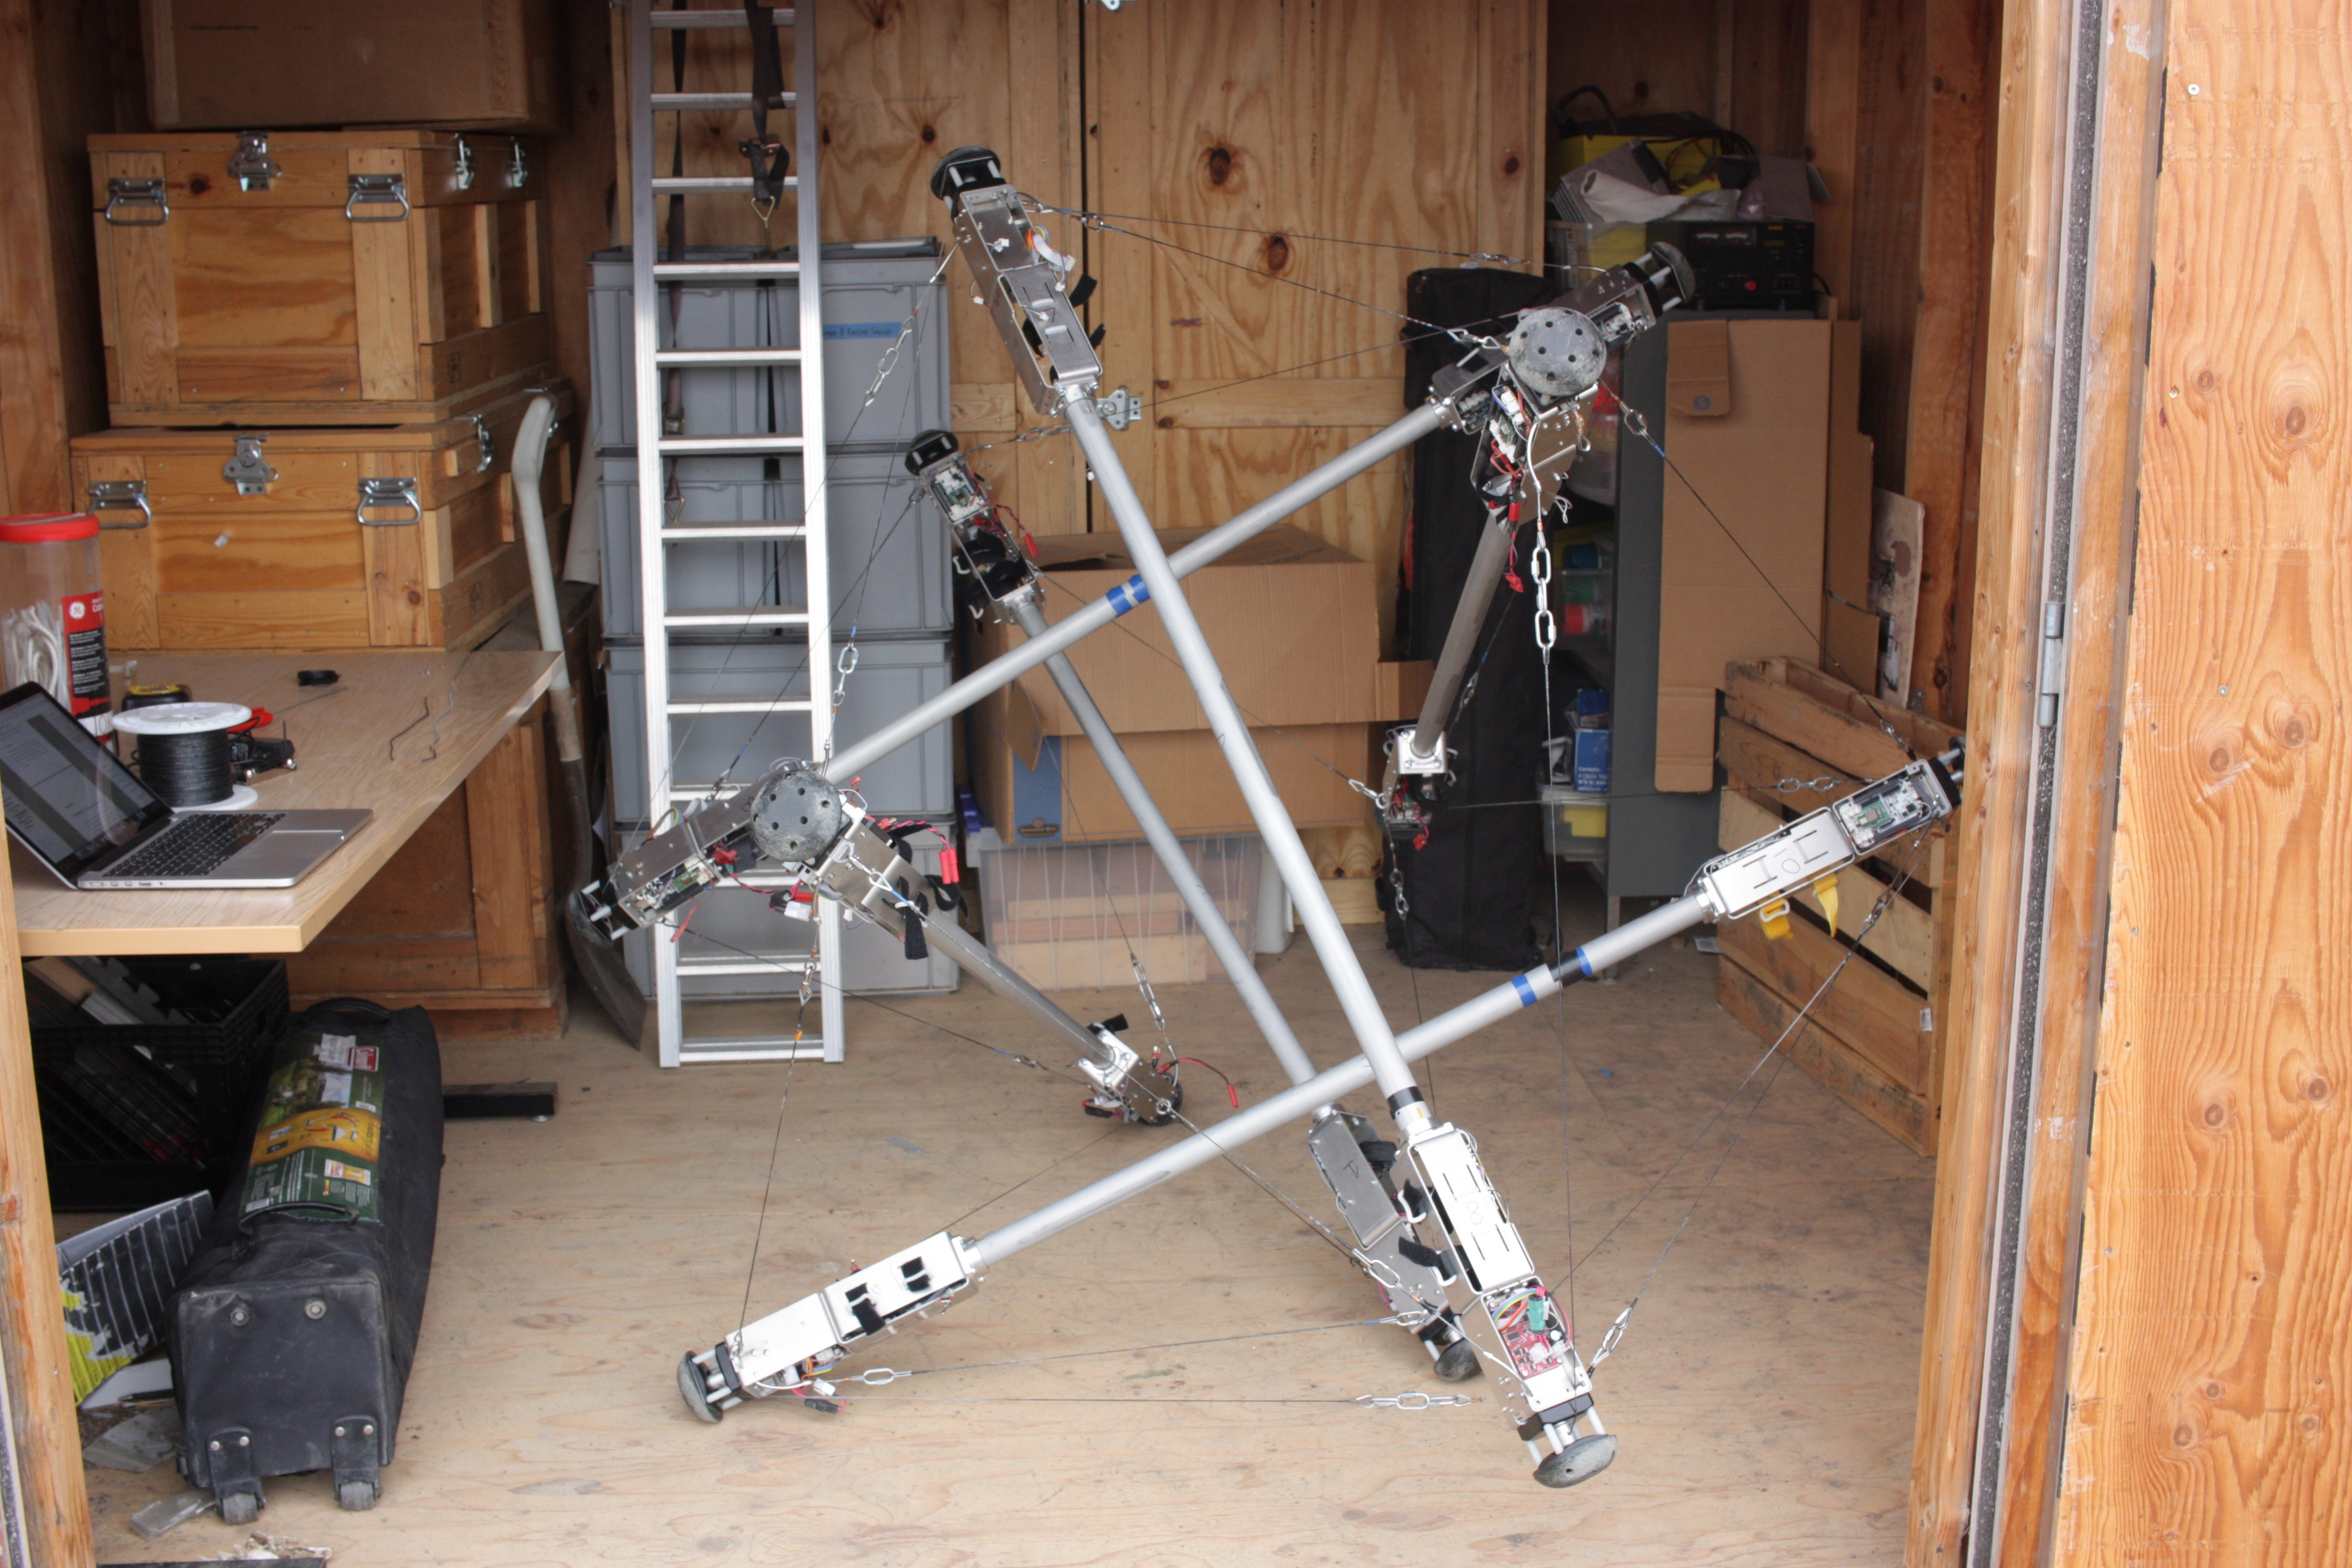
\includegraphics[width=0.9\linewidth]{tex/img/full_sb_up}%
\label{fig:sb_up}%
\caption{}
\end{subfigure}%
\begin{subfigure}{.5\textwidth}
\centering
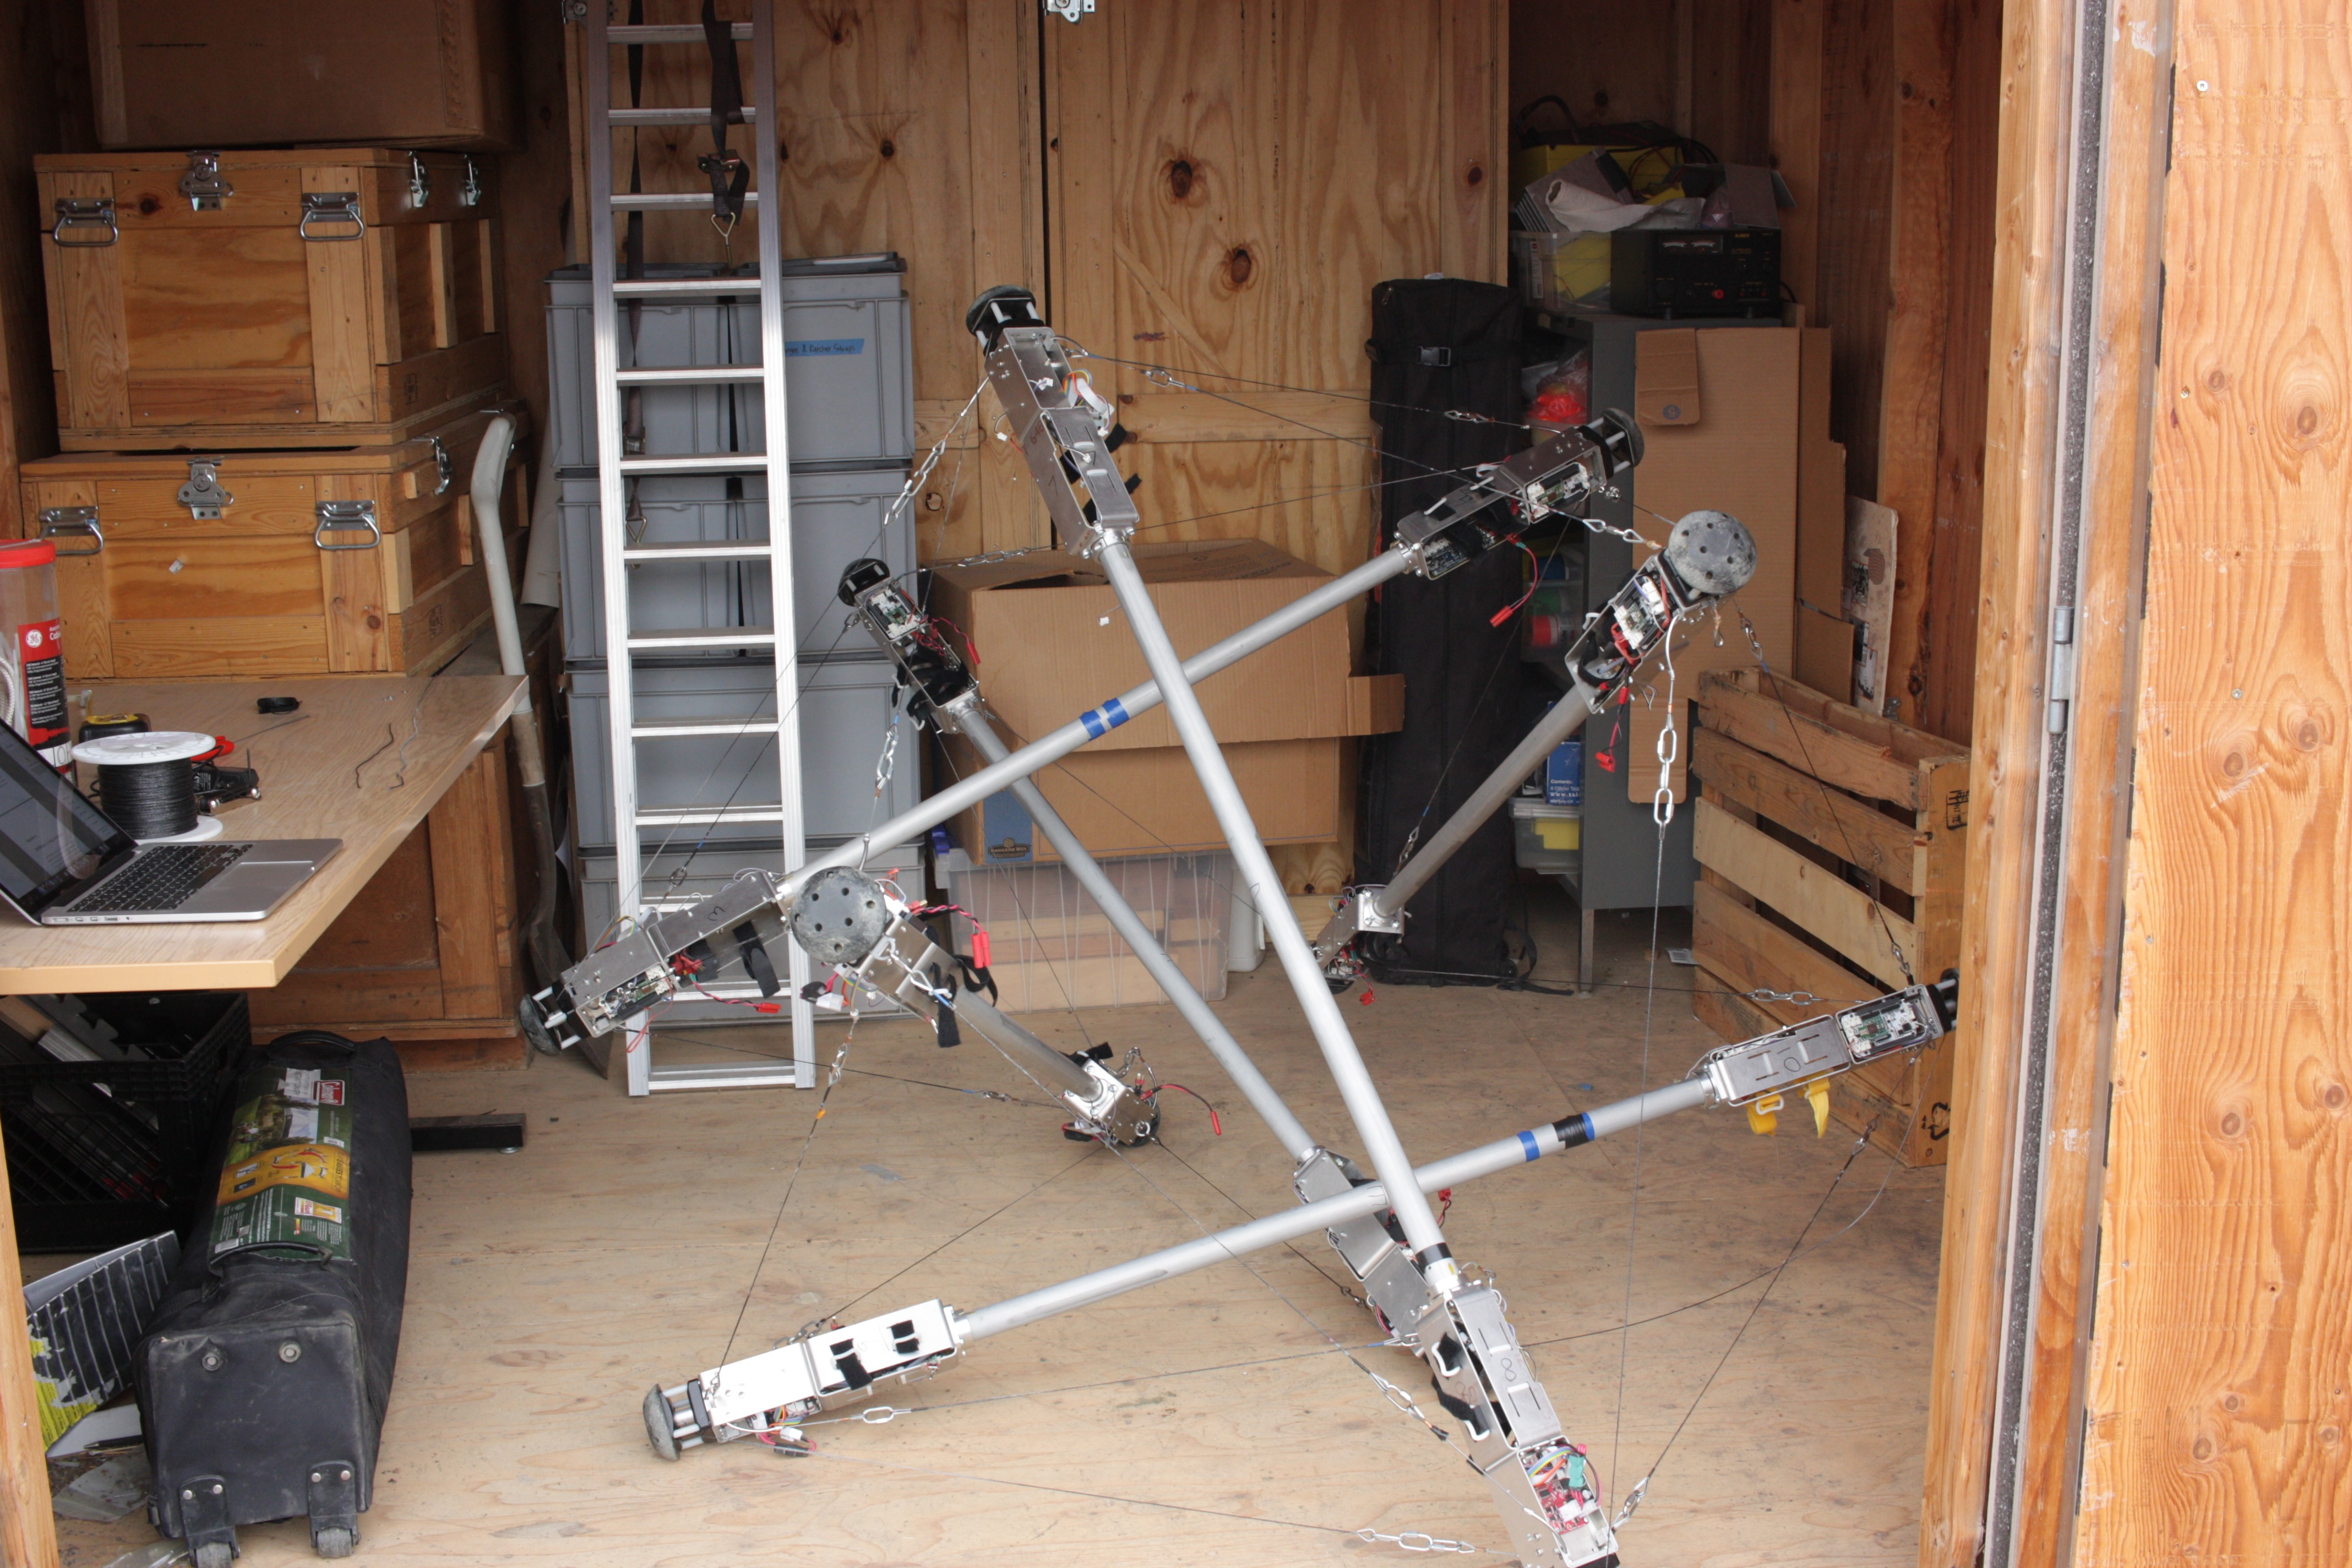
\includegraphics[width=0.9\linewidth]{tex/img/full_sb_down}%
\label{fig:sb_down}%
\caption{}
\end{subfigure}%

\caption{These figures show the hystresis effect due to friction on the \SB{}. \SB{} in the (a) figures has been lifted off the ground and gently placed back down so that all the springs in the system are allowed to reach equilibrium due to gravity. No extra force has been placed on the robot other than gravity. \SB{} in the (b) figures was arbitrarily pushed downwards on two of the top endcaps with enough force to deform the robot. It can easily been seen the that the internal friction does not allow for the robot to return to it's original state.}
\label{fig:cable_friction}
\end{figure}

Another limitation imposed by the cable routing system was the lack of design effort that went into the cable exit system.
Originally, it was designed to be a section of the nylon bowden cable housing sticking out of the robot to isolate the steel cable as it exited the MTR aluminum housing.
However, the angle in which the cable exits the system was never considered in the original \SB{} design. 
This failure meant that an exit angle of 90 degrees perpendicular to the rod as used for the cable exit.
Comparing this to the actual cable exit angle of approximately 30 degrees from perpendicular during normal operation meant that more than \(60\%\) of the tension force is imparted into the nylon cable and the aluminum housing exit hole.
When the cable would slide in and out of the exit point, the nylon tube quickly would sheer apart.
This then caused the steel cable to rub on the aluminum housing, which then would slowly saw into the housing.
Since there was not budget to redesign the whole routing system, a drop in replacement fix was required. 
The solution was to use a "break noodle" steel cable router typically used in bicycle braking systems.
This prevented the steel cable from cutting into to MTR housing, but it causes a bit more friction to get imparted into the whole cable system.
Figure~\ref{fig:cable_output} shows the cable exit point on \SB{} with the "break noodle" fix.

\begin{figure}[thpb]
      \centering
      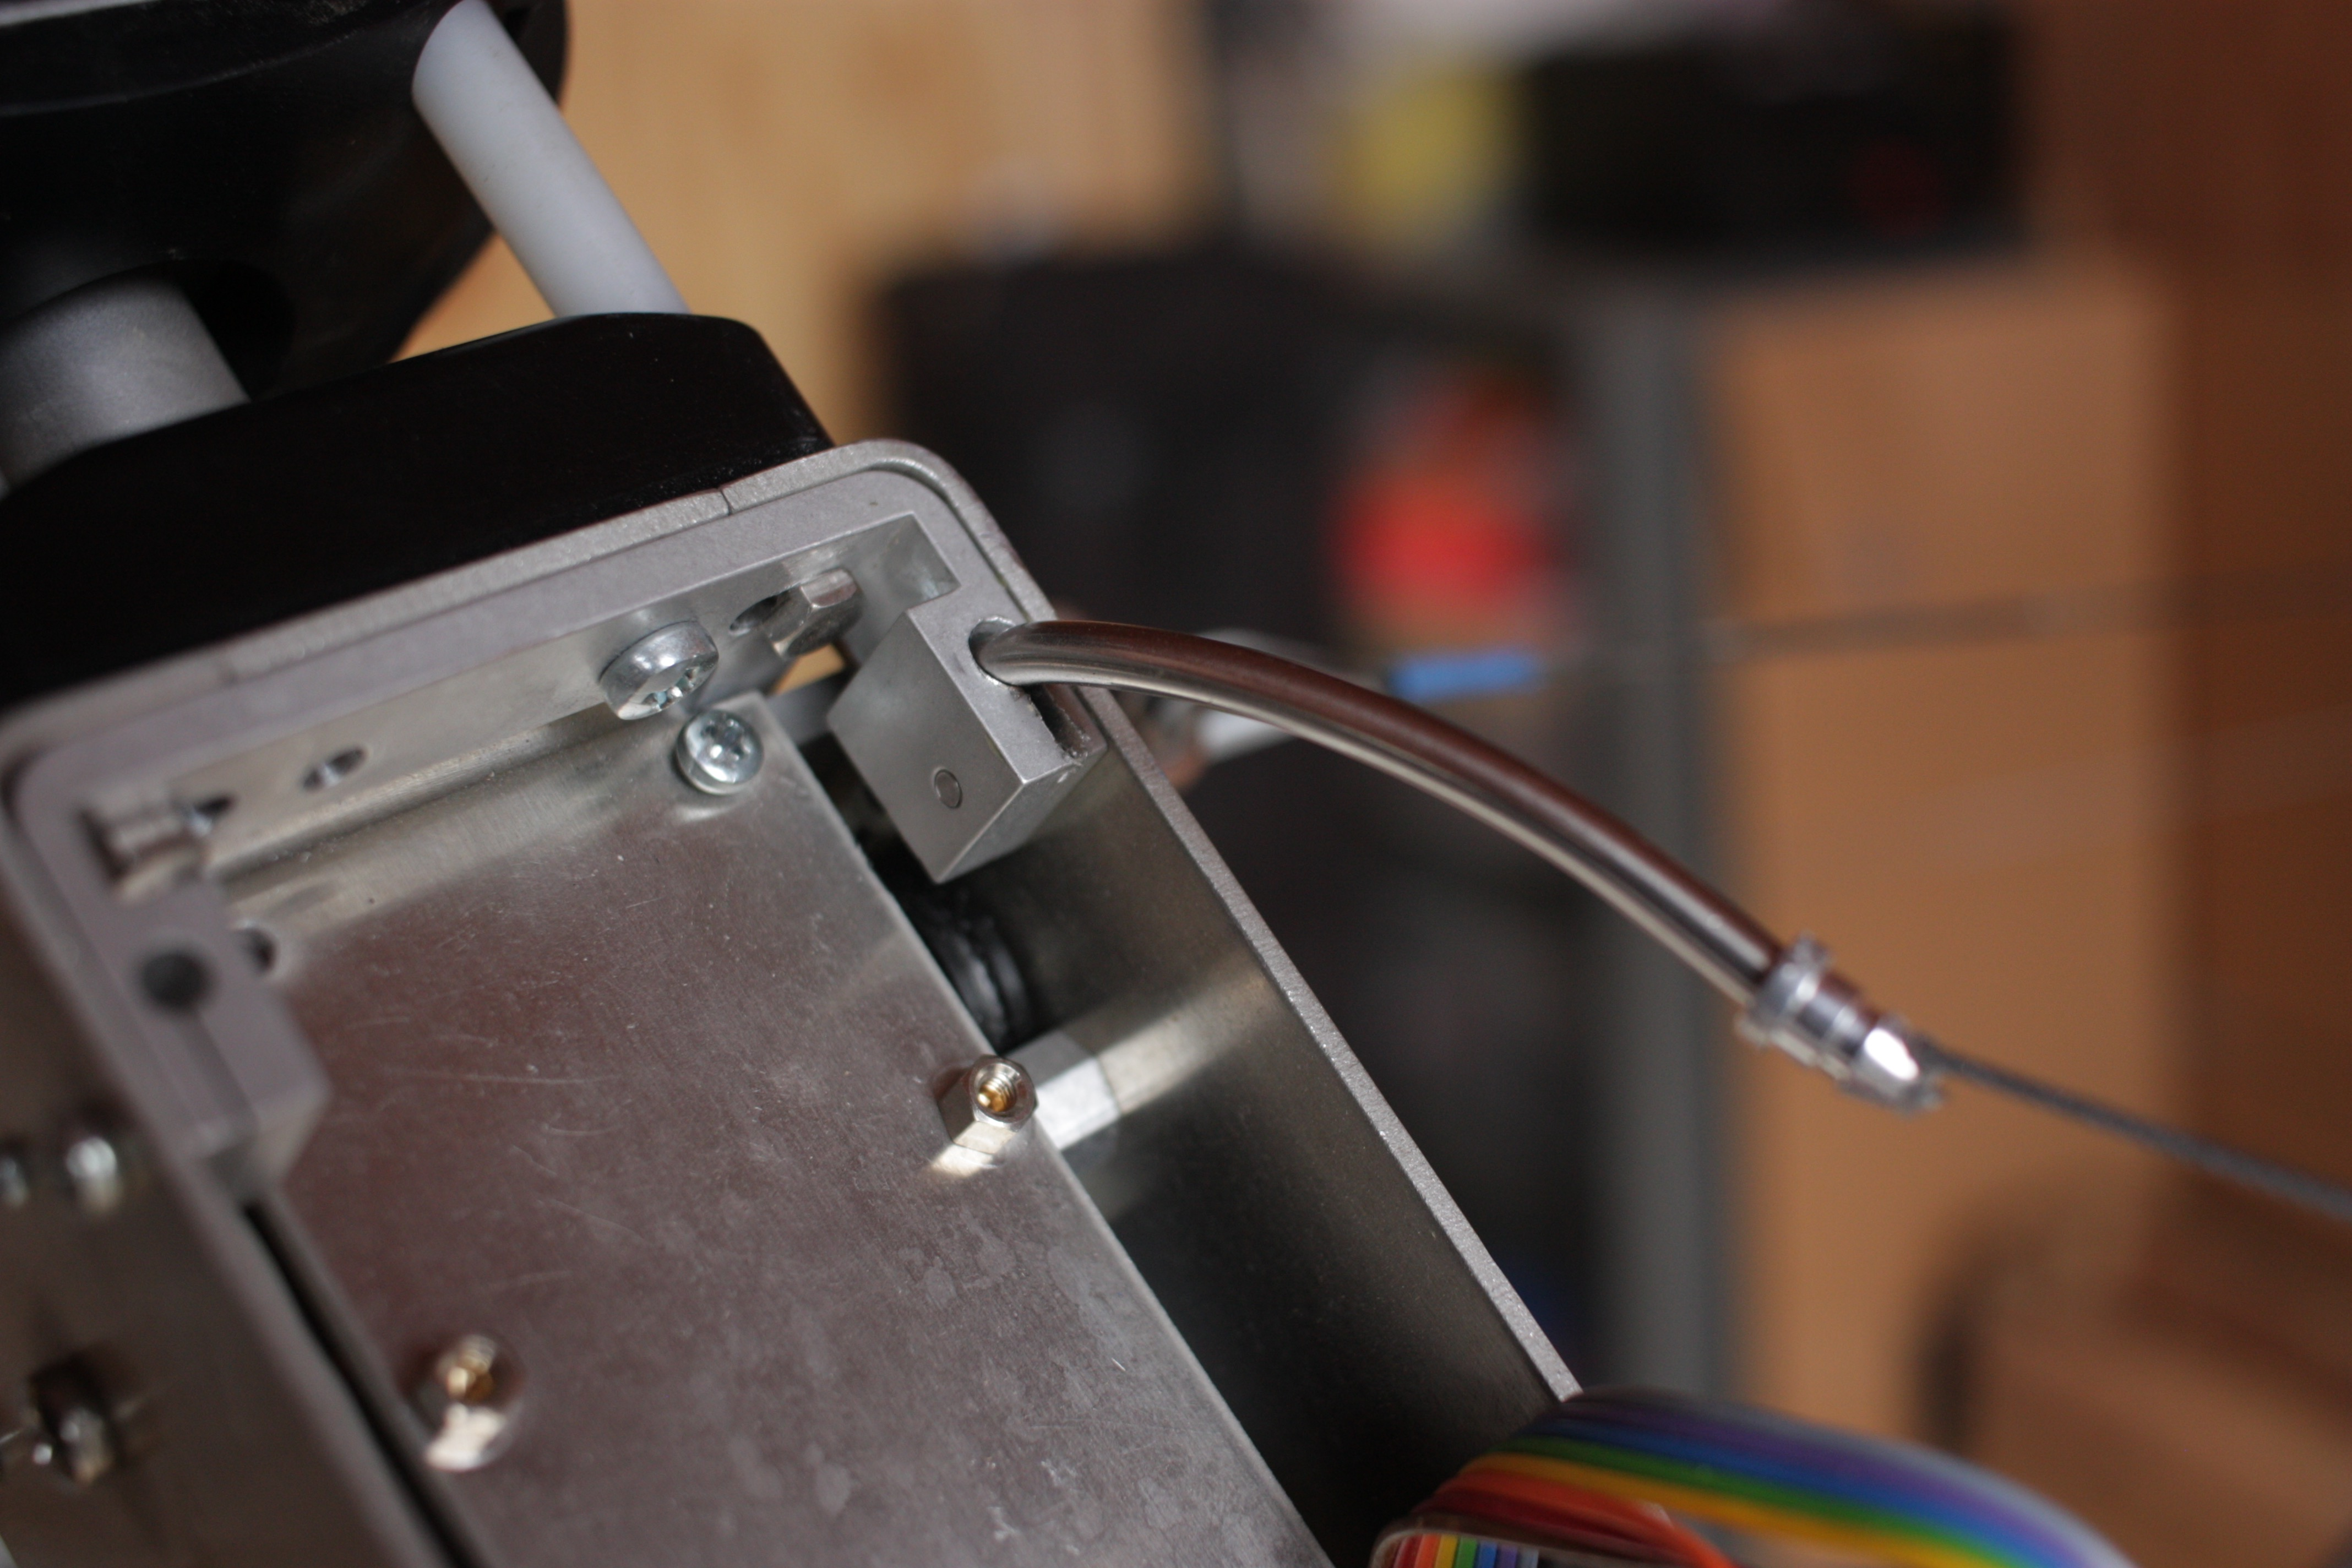
\includegraphics[width=0.8\columnwidth]{tex/img/bracket_cut}
      \caption{This figure shows the original exit point for the steel cable on \SB{} with the "break noodle" fix. The point of entry of the "break noodle" is can be seen where the aluminum of the bracket has been cut by the steel cable before the fix was applied.}
      \label{fig:cable_output}
\end{figure}

\subsection{Cable Tension}
\label{sec:cable_tension}
Another limitation on the system's performance is the larger than designed tensions seen on the individual cables.
This caused a limit on the maximum length each actuator imposes on a cable. 
Max cable tension on \SB{} was designed around a maximum continuous operating tension force of \(200N\) per cable.
The system was also designed to take intermittent forces \(50-75N\) higher than this maximum that would be caused by rolling.
These values were obtained through evaluating the tension forces derived from Iscen et al's control work within the NASA Tensegrity Robotics Toolkit~\cite{iscen2014flop}.
Atil used a simulated robot based on the initial design of \SB{}, which consisted of a total mass of \(18kg\) and each rod being \(1.5m\) in length. 
Comparing these values to those in table~\ref{design_req}, the final \SB{} parameters were different than the ones used to determine the operating tensions.
This was due to Atil's work was published quite early in the design process and not all the mechanical design aspects of the MTRs were finalized.
This discrepancy in weight caused the actual nominal operating tension to be around \(240N\) and the maximum operational tension to be above \(400N\).

The motors used in the final design of \SB{} were 100 watt Maxon motors as specified in table~\ref{motor_parameters}.
Each motor has a Maxon gearbox with a maximum continuous output torque of \(3Nm\) originally designed to be coupled to a spool with a diameter of \(30mm\).
Using the spool's radius and the robot's operating tensions listed above, the reaction torques applied to the gearboxes are calculated in equations~\ref{tau_nom} and~\ref{tau_max}.

\begin{align}
\tau_{nominal, 30mm} = 240N \times 0.015m = 3.6Nm \label{tau_nom} \\
\tau_{maximum, 30mm} = 400N \times 0.015m = 6.0Nm \label{tau_max}
\end{align}

These values are well above the continuous and peak torques that the motor's gearbox is rated to handle.
To keep from breaking all the motors when operating the robot, smaller diameter spools were designed. 
The trade off is that the cable actuation velocity is decreased, forcing the robot to move slower.
Decreasing the cable actuation velocity too far will result in a robot which will be incapable of achieving a continuous average forward velocity.
At the time, the only controller which moved a simulated \SB{} like robot with a continuous velocity was Iscen's work, which required a cable actuation velocity of \(30 cm/s\)~\cite{iscen2014flop}.
Thus reducing the speed below \(50\%\) could potentially be too slow to achieve continuous forward velocity.
The new spindles were then reduced to a spool diameter of \(18mm\) and the new torques are shown in equations~\ref{new_nom} and~\ref{new_max}.

\begin{align}
\tau_{nominal, 18mm} = 240N \times 0.009m = 2.7Nm \label{new_nom} \\
\tau_{maximum, 18mm} = 400N \times 0.009m = 3.6Nm \label{new_max}
\end{align}

This design still is not ideal, but is a compromise between reducing the reaction torque on the gearboxes and not reducing the actuation velocity too low.
The torques induced onto the gearbox could still go over the rated value during maximum tension scenarios, but reduces the actuation speed to \(47\%\) of the original value set by Iscen.
To further reduce the reaction torques applied to the gearboxes, a maximum position of cable change was set to keep the reaction torque applied my any one motor to be within the nominal spool reaction torque in equation~\ref{new_nom}.
Though experimentation, the limit was found to be \(40cm\) of cable change from a pretension value in each cable of \(100N\).

\subsection{Cable Material}
The choice of external cable material used on \SB{} made some complications in the long term use of the system.
The material used is a \(1.3mm\) diameter braided hollow core Vectran cable.
This cable has excellent material properties for a system which requires light and strong cables with near zero creep.
However, the cable has a high coefficient friction and will undergo tensile fractures when exposed to large amounts of stress.
This causes the many thin fibers to fray, eventually leading to loss in overall tensile strength and eventual failure. 
In \SB{}, this usually occurs at the cabling closest to the spool. 
Since this small length of cable always experiences high stress due to wrapping around the spool, the cables fray quite rapidly and break.
The frequency of this happening depends on how many times that particular cable is used.
On average it has become an expectation that a single cable will break after at least three hours of actuation on that single cable. 
Figure~\ref{fig:cable_break} shows different stages of the vectran cable as it wears to breakage.

\begin{figure}[thpb]
      \centering
      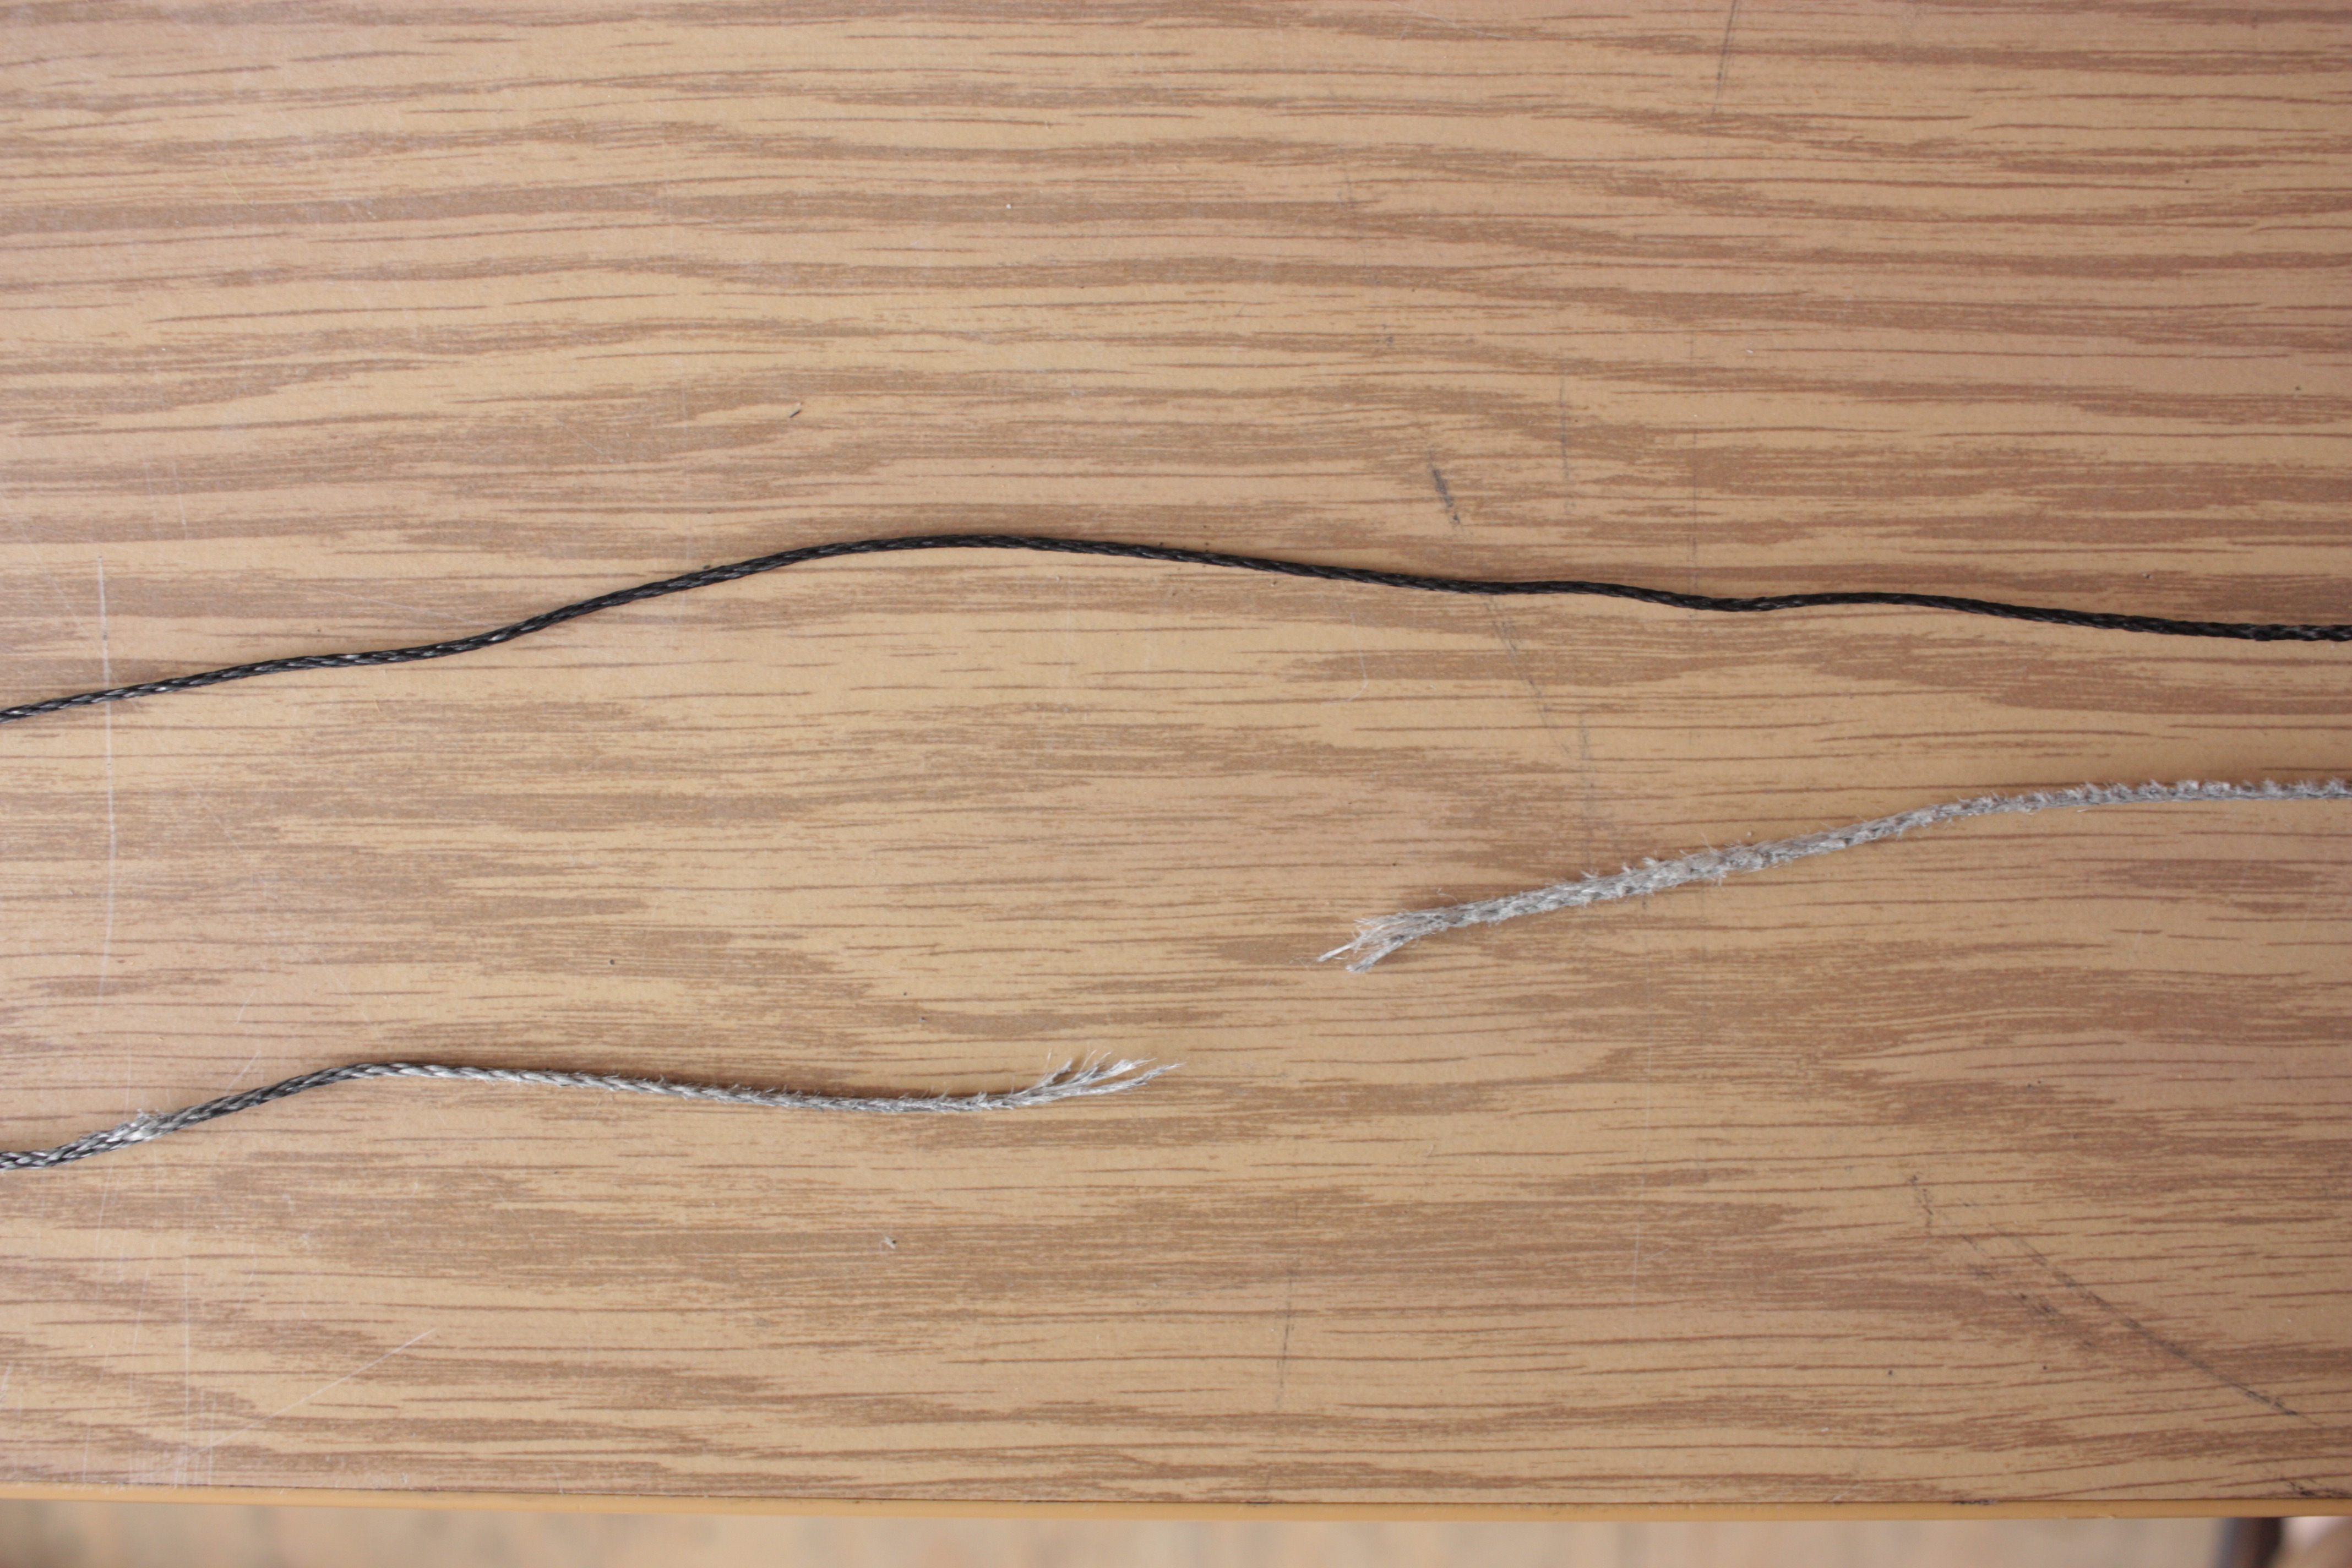
\includegraphics[width=0.8\columnwidth]{tex/img/broken_cable}
      \caption{This figure shows how wear on the cable. The vectran cable's protective outer coating wears off during use which then allows for the individual fibers to break weakening the entire cable. Eventually this wear will degrade the max holding tension to the point of failure. The black cable is a new vectran cable and the cable below shows the black coating worn away and a breakage point. The bottom cable is from an actual failure on the system during a run. Since the system can absorb forces, when the cable breaks the stored energy gets distributed into the robot and no violent backlash is experienced.}
      \label{fig:cable_break}
\end{figure}

\subsection{Force Sensors}
\label{force_sensing_failure}
\SB{} was designed to have three force sensors per MTR system to sense forces being applied by the motor, the distal actuated cable, and the distal passive cable.
Since the system had a constrained budget, purchasing off the shelf force sensors was out of the budget and custom sensors were implemented.
Figure~\ref{fig:force_sensors} shows the designs for each force sensor.

\begin{figure}[thpb]
      \centering
      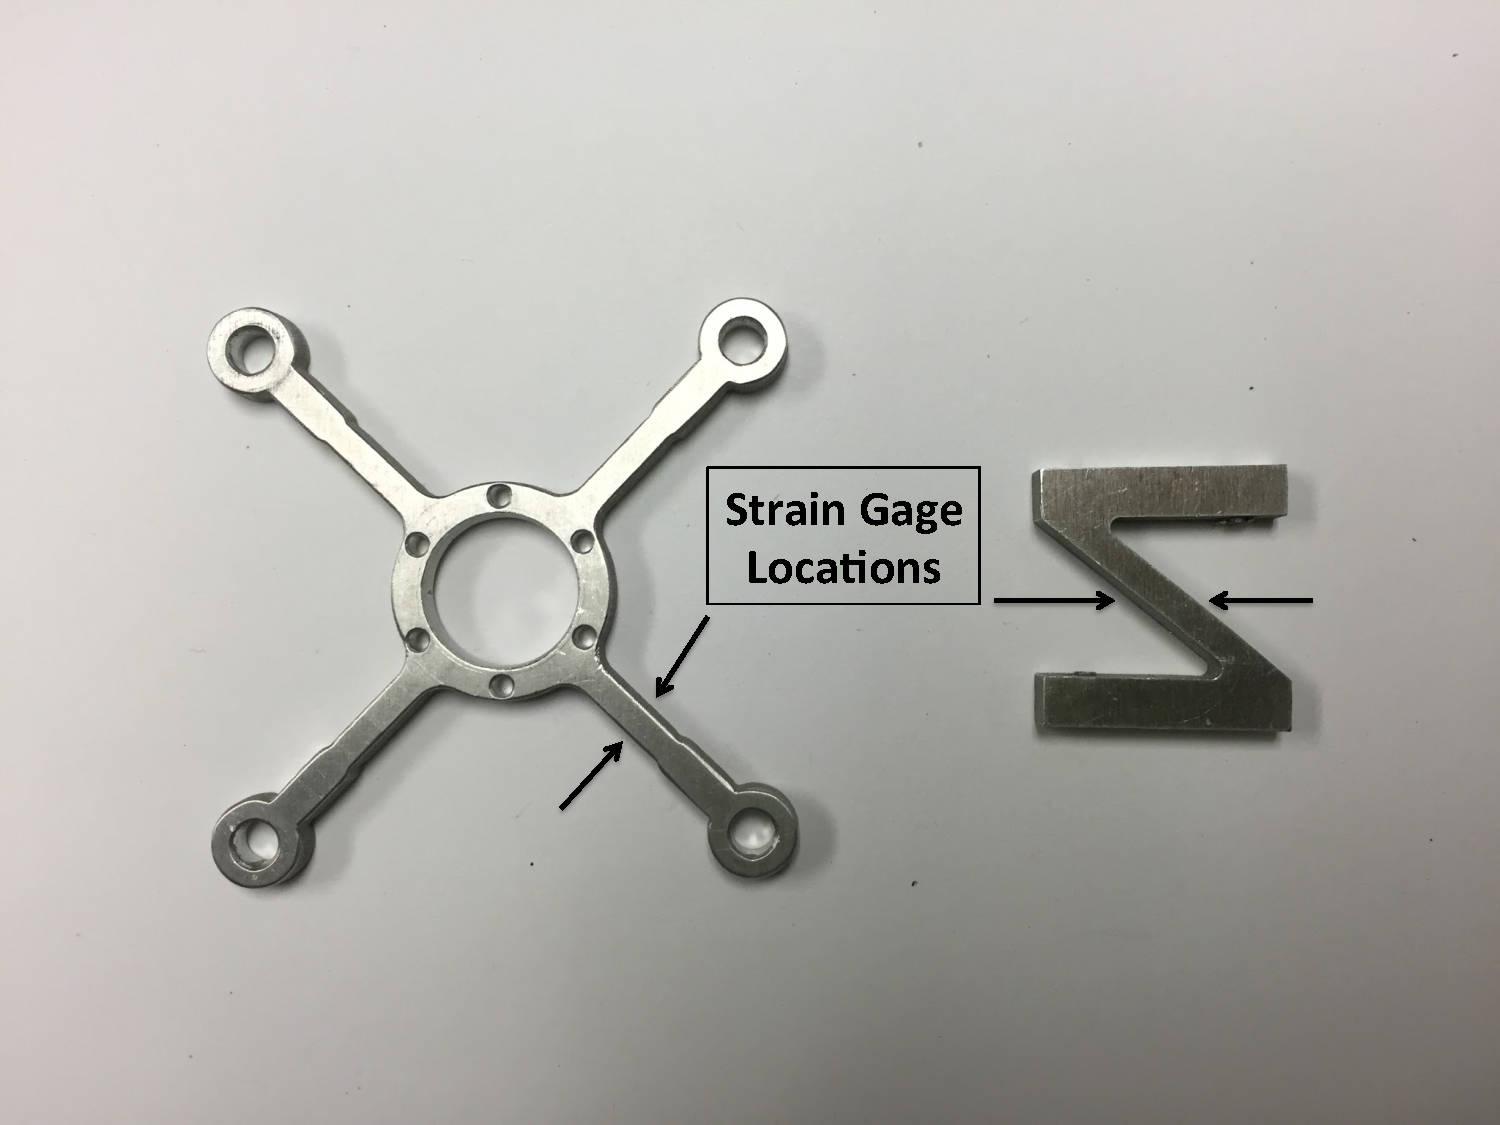
\includegraphics[width=0.8\columnwidth]{tex/img/strain_gages}
      \caption{This figure shows the designs for the motor mount strain gage and the spring strain gage. The motor mount is located on the left, and it functions when the arms of the cross beams deform due to the reaction torque caused by torque being applied to the motor. The right shows the original design for the spring sensors. This gage is suppose to sit between the spring and the ridged mount and compress due to spring force. However, the design never worked.}
      \label{fig:force_sensors}
\end{figure}

\paragraph{Dynamic Torque Sensor Testing}
\begin{figure}[thpb]
      \centering
      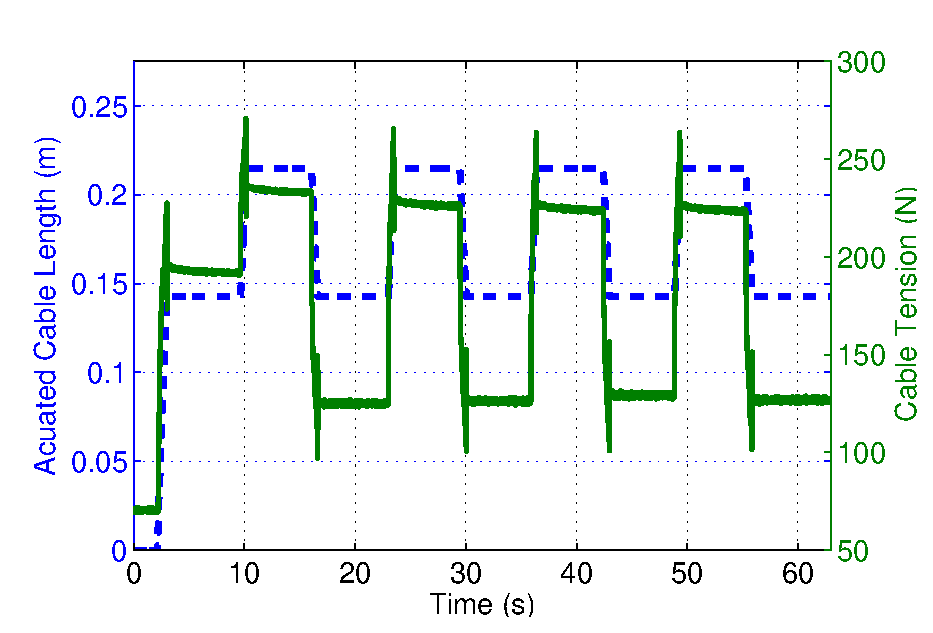
\includegraphics[width=0.8\columnwidth]{tex/img/ICRA2015_dynamic_sensor_test}
      \caption{Motor mount torque sensor data and motor position data recorded during a square wave input position trajectory for a single motor. This plot shows measured tension from the sensor and cable length from motor encoder measurements as a function of time for this dynamic movement.}
      \label{fig:sensor1data}
\end{figure}

This test was performed to demonstrate the force sensors' ability to capture data under dynamic motion.
Figure~\ref{fig:sensor1data} shows a plot of sensor data from one end cap whose motor is commanded in a square-wave position trajectory.
The position trajectory had a period of \SI{13}{\second}, and oscillated between \SI{10}{\radian} and \SI{15}{\radian} of the output shaft measured before the gearbox, by the encoder.
The trajectory of sensor torque values reasonably tracks the position square wave: the commanded position trajectory starts at 10 seconds and ends at 62 seconds, as does the sensed tension square wave.
The overshoot on the torque sensor measurements is due to the system inertia and spring dynamics.

\paragraph{Global Force Redistribution Sensor Testing}

A test was performed to validate the distribution of tension throughout the system, and to show that all sensors can work in conjunction simultaneously.
Figure~\ref{fig:sensor2data_forcedistribution} shows tension readings from a different motor-mount torque sensor on the opposite side of \SB{} (Cable 2) from a cable which is being retracted (Cable 1.)
Cable 2 was not actively actuated during each test.
For each plot in Figure~\ref{fig:sensor2data_forcedistribution}, the actuated cable was retracted with various step inputs marked in the figure.
Each data point in this figure (yellow) was collected by averaging data from the sensor board for a total of 5 seconds at 1 kHz, after waiting 2 seconds after the step input actuation to avoid dynamic effects.
These tests were done with different levels of pretension on the sensed cable: this pretension was adjusted by changing the length of the sensed cable.
Though the lower-pretension tests show smaller changes in readings, the higher pretensions show increasing readings which demonstrate the ability to sense forces throughout the tension network in pseudo-equilibrium states, as well as \SB{}'s passive force redistribution properties.

\begin{figure}[thpb]
      %\vspace{-0.5cm}
      \centering
      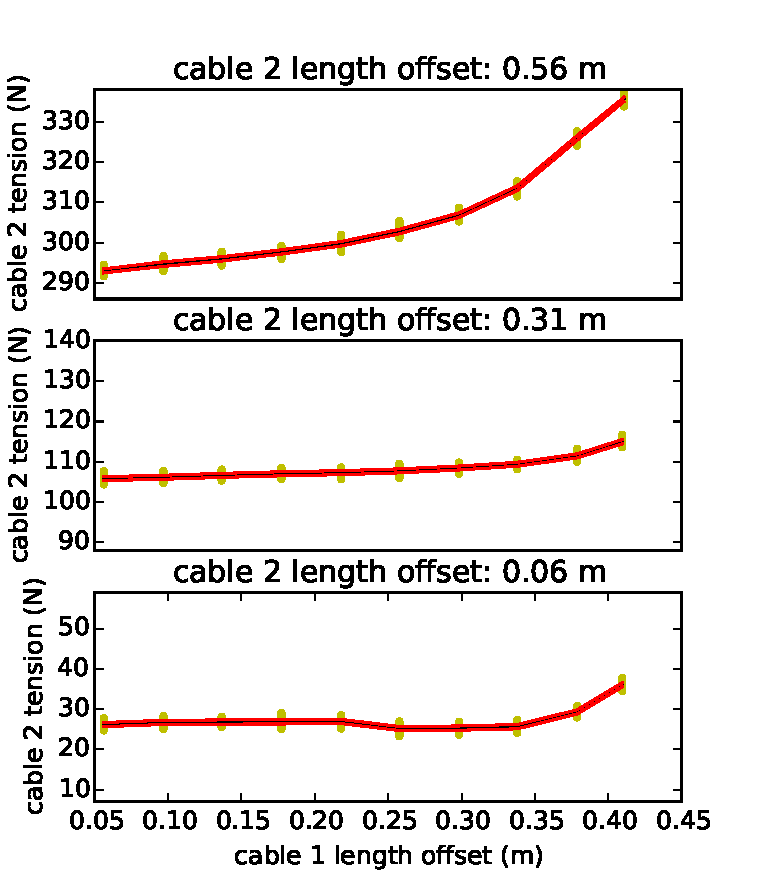
\includegraphics[width=0.55\columnwidth]{tex/img/sensor2_original}
      \caption{Global force redistribution test. Yellow marks are the means of roughly 5,000 tension sensor measurements of \emph{cable 2} opposite that which is actuated (\emph{cable 1}.) The black line shows the linear interpolation between points, with the red boundary as standard deviation. The pretension in the sensed cable is adjusted in each test, showing measurement sequences at increasing pretensions.}
      \label{fig:sensor2data_forcedistribution}
\end{figure}

\paragraph{Force Sensing Viability}
The force reaction sensor was the only custom sensor to accurately sense the forces applied.
However, inconsistencies in manufacturing this sensor made calibration of each sensor extremely difficult.
This coupled with not being robust to handling, it was extremely difficult to get all twelve sensors working at one time.
A single sensor could be made, calibrated and functional for about a day or two after which the sensor's strain gages would shift.
This either would making the calibration no longer valid or be such an shift, that the sensor would no longer be functional.
Due to these set backs, the force sensors were disregarded as viable sensors to be used on the system.

\section{Electrical Evaluation}

\subsection{Sensor Board}
The sensor board eventually functioned as designed.
All major functions that were set out in its inception were implemented.
It was able to deliver the CAN physical layer for the Beagle Bone Black, interpret and condition sensor data, and enable the addition of the DWM module (which was not in the initial design).
The only caveat in its sound function was driver code developed for the DWM module.
If the DWM module crashed, usually due to the inability to handle soft system resets, the SPI communication line would block the sensor board code.
This was a rare occurrence, but would require a full power cycle of the sensor board to recover.
The correct fix is to implement the DWM module's SPI code to be non-blocking, however this was not a higher priority than finishing other higher level control experiments.

\subsection{Power Board}
This board was the "heart" of \SB{} and functioned extremely well.
It distributed conditioned power to all electronics and sensors on \SB{} as well as managed many of the safety features on \SB{}.
One down side to this board was its size.
Since it has many complex features implemented in discrete logic, the board has 136 components.
This made the board expensive and large, with some extra features which were never utilized in the final implementation of \SB{}.
To improve upon this, designing the board as a two sided PCB would reduce the size dramatically.
Furthering reducing the size and complexity would be to not support 6 power lines.
These were originally implemented to support expansion boards.
However, this feature was never utilized and in hind sight would never need to support that many extra boards.

\subsection{Motor Board}
For the most part, all the electronic boards on \SB{} functioned as designed with only the motor control board having lasting issues that hindered the performance of the system.
The motor board was suppose to be a low cost solution to achieve position, velocity, and torque control utilizing the Field Oriented Control (FOC) method to commutate the brushless DC motors.
A third party start-up company was tasked with the design of the motor board.
It took the company many attempts to get a working version for just position control, with the initial delivery causing motors to generate excessive heat due to shorting the windings during commutation.
After a quick redesign and manufacturing new boards, position control was achieve with pretty good results.
However, the company went out of business after their delivery of working motor control boards and never completed their implementation of the other control methods.
This in conjunction with the issues stated in section~\ref{force_sensing_failure}, torque control was never implemented.

% The main feature of the sensor board was to monitor and control any of the sensors required on \SB{} by a dedicated processor.
% This was to insure that none of the critical safety features would be hindered by sensor tasks.
% Most of the board's functions work as expected.
% %However the analog to digital converter became useless after all the force sensors failed as explained in section~\ref{force_sensing_failure}.
% The only real issue when using this board steams from the re-purposing of the XBee WiFi headers for controlling a DecaWave DWM1000 module.
% This placed the module's antenna too close to the robot to effectively get ranging data in all directions.
% A better design would have place the antenna such that one complete side of the sensor was not completely blocked by the MTR module. 


% \subsection{Motor Board}
% The motor control board for \SB{} never worked as designed and eventually limited the capabilities of the system.

\section{Communications Evaluation}
There were two main types of data communication on \SB{}, a CAN bus and the wireless WiFi network enabled on each rod.

\subsection{CAN Bus}
Since \SB{} was designed to have multiple boards communicating on a single network over distances greater than one meter, a CAN bus was implemented to achieve these goals.
For the most part, this network along with the CANOpen standard met all of the initial design criteria.
However, sending a small number of messages at \(\SI{1}{\kilo\hertz}\) would over flow the bus at the maximum network speed of \(1 Mbit/s\).
This is in part due to the large CANOpen message header and the large data types bing transmitted.
The protocol also uses a lot of system resources to manage.
It was measured that approximately \(10\%\) of the micro controllers' total computation went into handling CAN messages.

\subsection{WiFi Network}
\SB{} relied upon standard WiFi communication through ROS to transmit data from the robot to an external computer on the network.
ROS messaging is extremely convenient for data logging, management, and conditioning all shared over a common network.
The main issue experienced with this implementation on \SB{} is due to the ARM based network driver support and WiFi dongles used.
These issues result in unexpected network lags and connection issues to the network.
Several driver and module addition were required to get the WiFi communication on the Beagle Bone Blacks to be stable and with a relative low network latency.
However, these fixes never solved the network connection issue.

The maximum range of the system was also limited due to the budget home router used.
Since purchasing though a government entity put limits on computer hardware, it was difficult to find a good wireless router which fit the design needs and budget.
Therefore, a budget router was purchase and the routing feature on the wireless router was disabled.
In its place, a Linux computer was setup as the router.
The budge wireless router (now a wireless access point), had a very weak signal and limited the systems range to about \(\SI{12}{\meter}\) in an open space.

% \textcolor{red}{
%  - CAN Bus 
%    > too slow for fast control and lots of data
%    > large overhead for processors utilizing driver code (CANOpen)
%  - BBB
%    > slow to boot
%    > draws lots of power
%    > Wifi dongle has connection issues
%    > big and heavy for what the board does
% }

\end{appendices}


% Outline
% Intro about tensegrities. Explain what the structure is and why it is important. Good to mention ideal tensegrities, class system, and prior robots and research.
% Modeling: This section will be a short section on basic linear modeling of a tensegrity structure. Mention that this is not my work, but and explination of prior research. 
% Mechatronics: This will be the longest section. Start off by talking about NIAC and the NASA proposal. Then move to how that directed over arching desgin goals. Move to then talk about the design matrix for SUPERball and how we choose some of the components that we did. Finish by explaining each major portion of the system.
% Results: This section will talk about the itial results from SUPERball. Tension information, motor power and control, battery monitoring, communication (ROS, CAN), 
% Future Work: Talk about where we are taking the project. Movement, learning, etc.

% Bibliography:
\clearpage
\bibliographystyle{unsrt}
\bibliography{final}

\end{document}
